\documentclass[12pt, oneside]{report}
\usepackage{sections/packages}
\usepackage{setspace}
\onehalfspacing


\geometry{a4paper, margin=1.2in}

\begin{document}
% \maketitle

\begin{titlepage}
\thispagestyle{empty} % No page number on title page
\centering
\vspace*{2cm}

{\LARGE\bfseries Zoobenthic Community Indicators of Sediment Contamination\par}
\vspace{1.2cm}

\end{titlepage}


% \clearpage

% \thispagestyle{empty} % No page number on abstract page
% \begin{center}
%     {\Large \textbf{Abstract}}
% \end{center}

% This is the abstract.


\clearpage
\pagenumbering{roman} % Use roman numerals for front matter
\setcounter{page}{1}
\tableofcontents

\clearpage
\pagenumbering{arabic} % Start Arabic numbering from first chapter
\setcounter{page}{1}   % Reset page counter to 1

\chapter{Introduction}

% \section{Study Background}
\section*{Key Model Parameters}

% ============================================================
% Global Pipeline Parameters (Model & Data Configuration Only)
% ============================================================
% Excludes: figure settings, output paths, saving options
% Suitable for Methods / Supplementary Methods section

\subsection*{Stage 1: Contamination Assessment}

\begin{table}[H]
\centering
\caption{Stage 1 -- Contamination Assessment Parameters}
\label{tab:stage1_params}
\begin{tabular}{l|l|p{6cm}}
\hline
\textbf{Parameter} & \textbf{Value} & \textbf{Description} \\
\hline
Transform method & log\_z\_score & Transformation applied to chemical variables \\
PC1 weight & 1.0 & Weight for principal component 1 \\
PC2 weight & 1.0 & Weight for principal component 2 \\
PC3 weight & 2.0 & Weight for principal component 3 (biologically relevant) \\
PC4 weight & 0.0 & Weight for principal component 4 \\
PC5 weight & 1.0 & Weight for principal component 5 \\
PC6 weight & 0.5 & Weight for principal component 6 \\
Save individual PCs & True & Save individual PC scores (PC1-PC6) \\
Standardize PCA scores & True & Standardize PC scores after PCA \\
Run RDA validation & True & Run RDA validation for pollution \\
RDA percentile threshold & 50 & Percentile for RDA reference sites \\
\hline
\end{tabular}
\end{table}

\subsection*{Stage 2: Taxa Assemblage on Reference Sites}

\begin{table}[H]
\centering
\caption{Stage 2 -- Taxa Assemblage Parameters}
\label{tab:stage2_params}
\begin{tabular}{l|l|p{6cm}}
\hline
\textbf{Parameter} & \textbf{Value} & \textbf{Description} \\
\hline
Reference percentile & 52\% & Bottom X\% of sites as reference (least polluted) \\
Species transformation & hellinger & Transformation method for species data \\
Number of clusters & 3 & Number of habitat clusters to identify \\
Top N taxa & 16 & Number of top taxa for visualizations \\
Linkage method & ward & Hierarchical clustering linkage method \\
Habitat variables & 6 & Environmental variables for habitat comparison \\
\hline
\end{tabular}
\end{table}

\subsubsection*{Habitat Variables (Stage 2)}
\begin{itemize}
\item Measured Depth (m)
\item Velocity at bottom (m/sec)\_Imputed
\item Water DO Bottom (mg/L)
\item Temperature (°C)
\item MPS (Phi)
\item LOI (\%)
\end{itemize}

\subsection*{Stage 3: Environment-Driven Taxa Clusters (RDA + LDA)}

\begin{table}[H]
\centering
\caption{Stage 3 -- RDA and LDA Parameters}
\label{tab:stage3_params}
\begin{tabular}{l|l|p{6cm}}
\hline
\textbf{Parameter} & \textbf{Value} & \textbf{Description} \\
\hline
RDA permutations & 999 & Number of permutation tests for RDA significance \\
LDA iterations & 1000 & Monte Carlo cross-validation iterations for LDA \\
Taxa transformation & hellinger & Species transformation for RDA \\
Top N taxa (RDA) & All & Top N taxa for RDA (None = all taxa) \\
RDA log-transform env & False & Log-transform environmental variables for RDA \\
RDA standardize env & True & Standardize environmental variables for RDA \\
LDA standardize env & True & Standardize environmental variables for LDA \\
LDA test size & 0.2 & Cross-validation test proportion \\
Random state & 42 & Random seed for reproducibility \\
\hline
\end{tabular}
\end{table}

\subsection*{Stage 4: Community Composition Ordination (PCA-based ZCI)}

\begin{table}[H]
\centering
\caption{Stage 4 -- Community Composition Parameters}
\label{tab:stage4_params}
\begin{tabular}{l|l|p{6cm}}
\hline
\textbf{Parameter} & \textbf{Value} & \textbf{Description} \\
\hline
Taxa transformation & hellinger & Species transformation method \\
Training percentile & 100.0\% & Percentage of sites to train PCA per cluster \\
Top N taxa & 16 & Number of top taxa in loading plots \\
PC variance threshold & 70\% & Cumulative variance for PC selection \\
Min PC variance & 5.0\% & Minimum variance threshold for regression analysis \\
Consistent taxa order & True & Use same taxa order across panels \\
Normalize PCs & False & Z-score normalize PCs for ZCI \\
ZCI computation method & least\_pollution\_threshold & Method for ZCI calculation \\
Least pollution threshold & 25\% & Bottom X\% as reference for ZCI \\
Ordination PC plane & (1, 2) & Principal components for ordination plot (PC1 vs PC2) \\
\hline
\end{tabular}
\end{table}



\chapter{Contamination Assessment}

\begin{figure}[htbp]
    \centering
    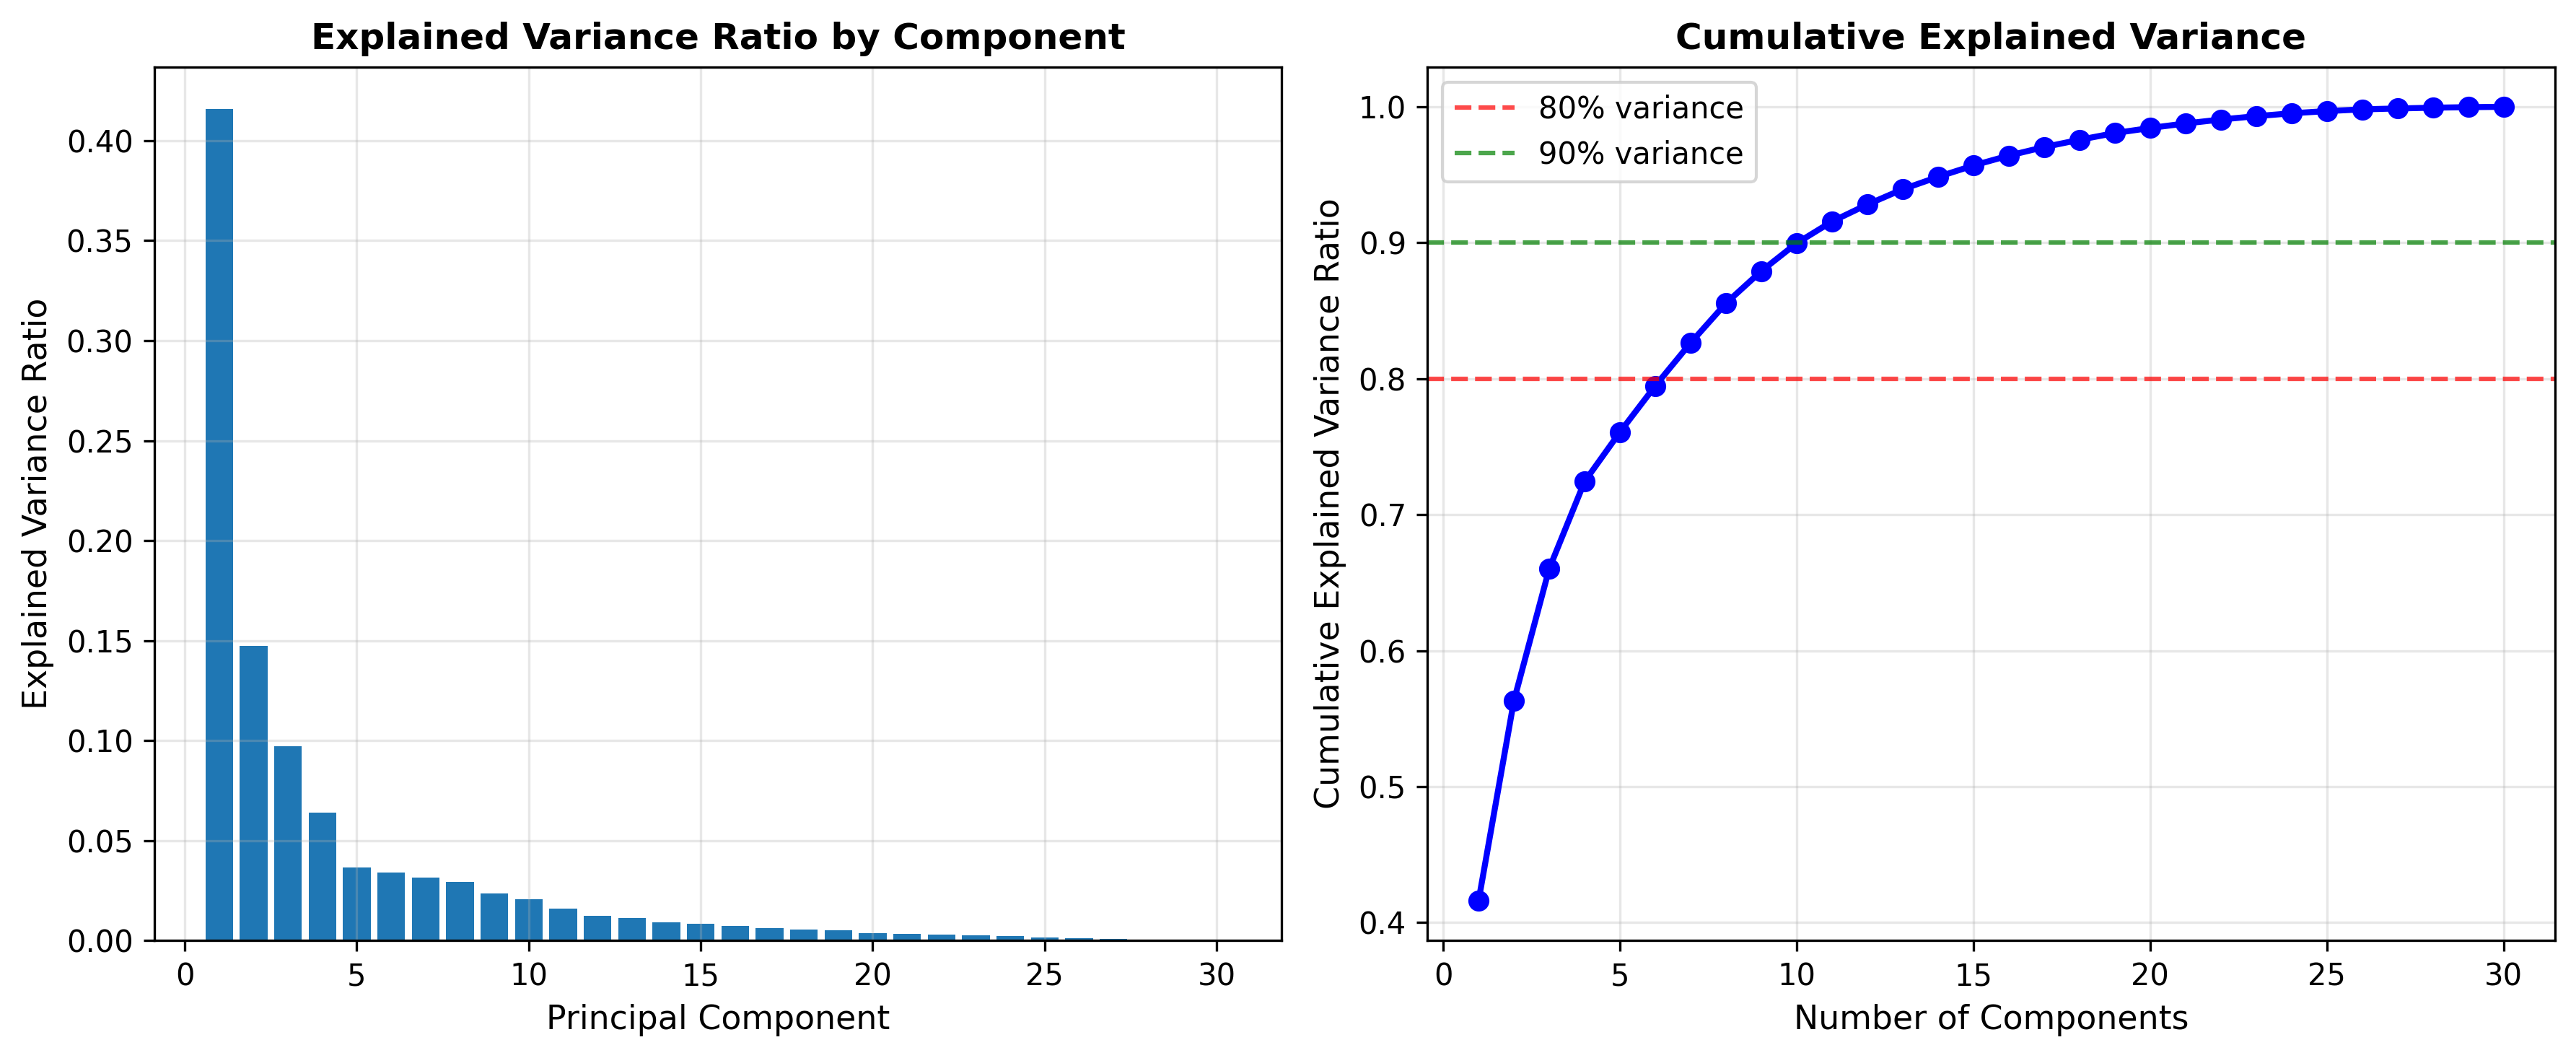
\includegraphics[width=0.9\textwidth]{../results/figures/01_contamination_assessment/figure1_pca_variance.png}
    \caption{PCA Variance}
    \label{fig:01_pca_variance}
\end{figure}

\begin{figure}[htbp]
    \centering
    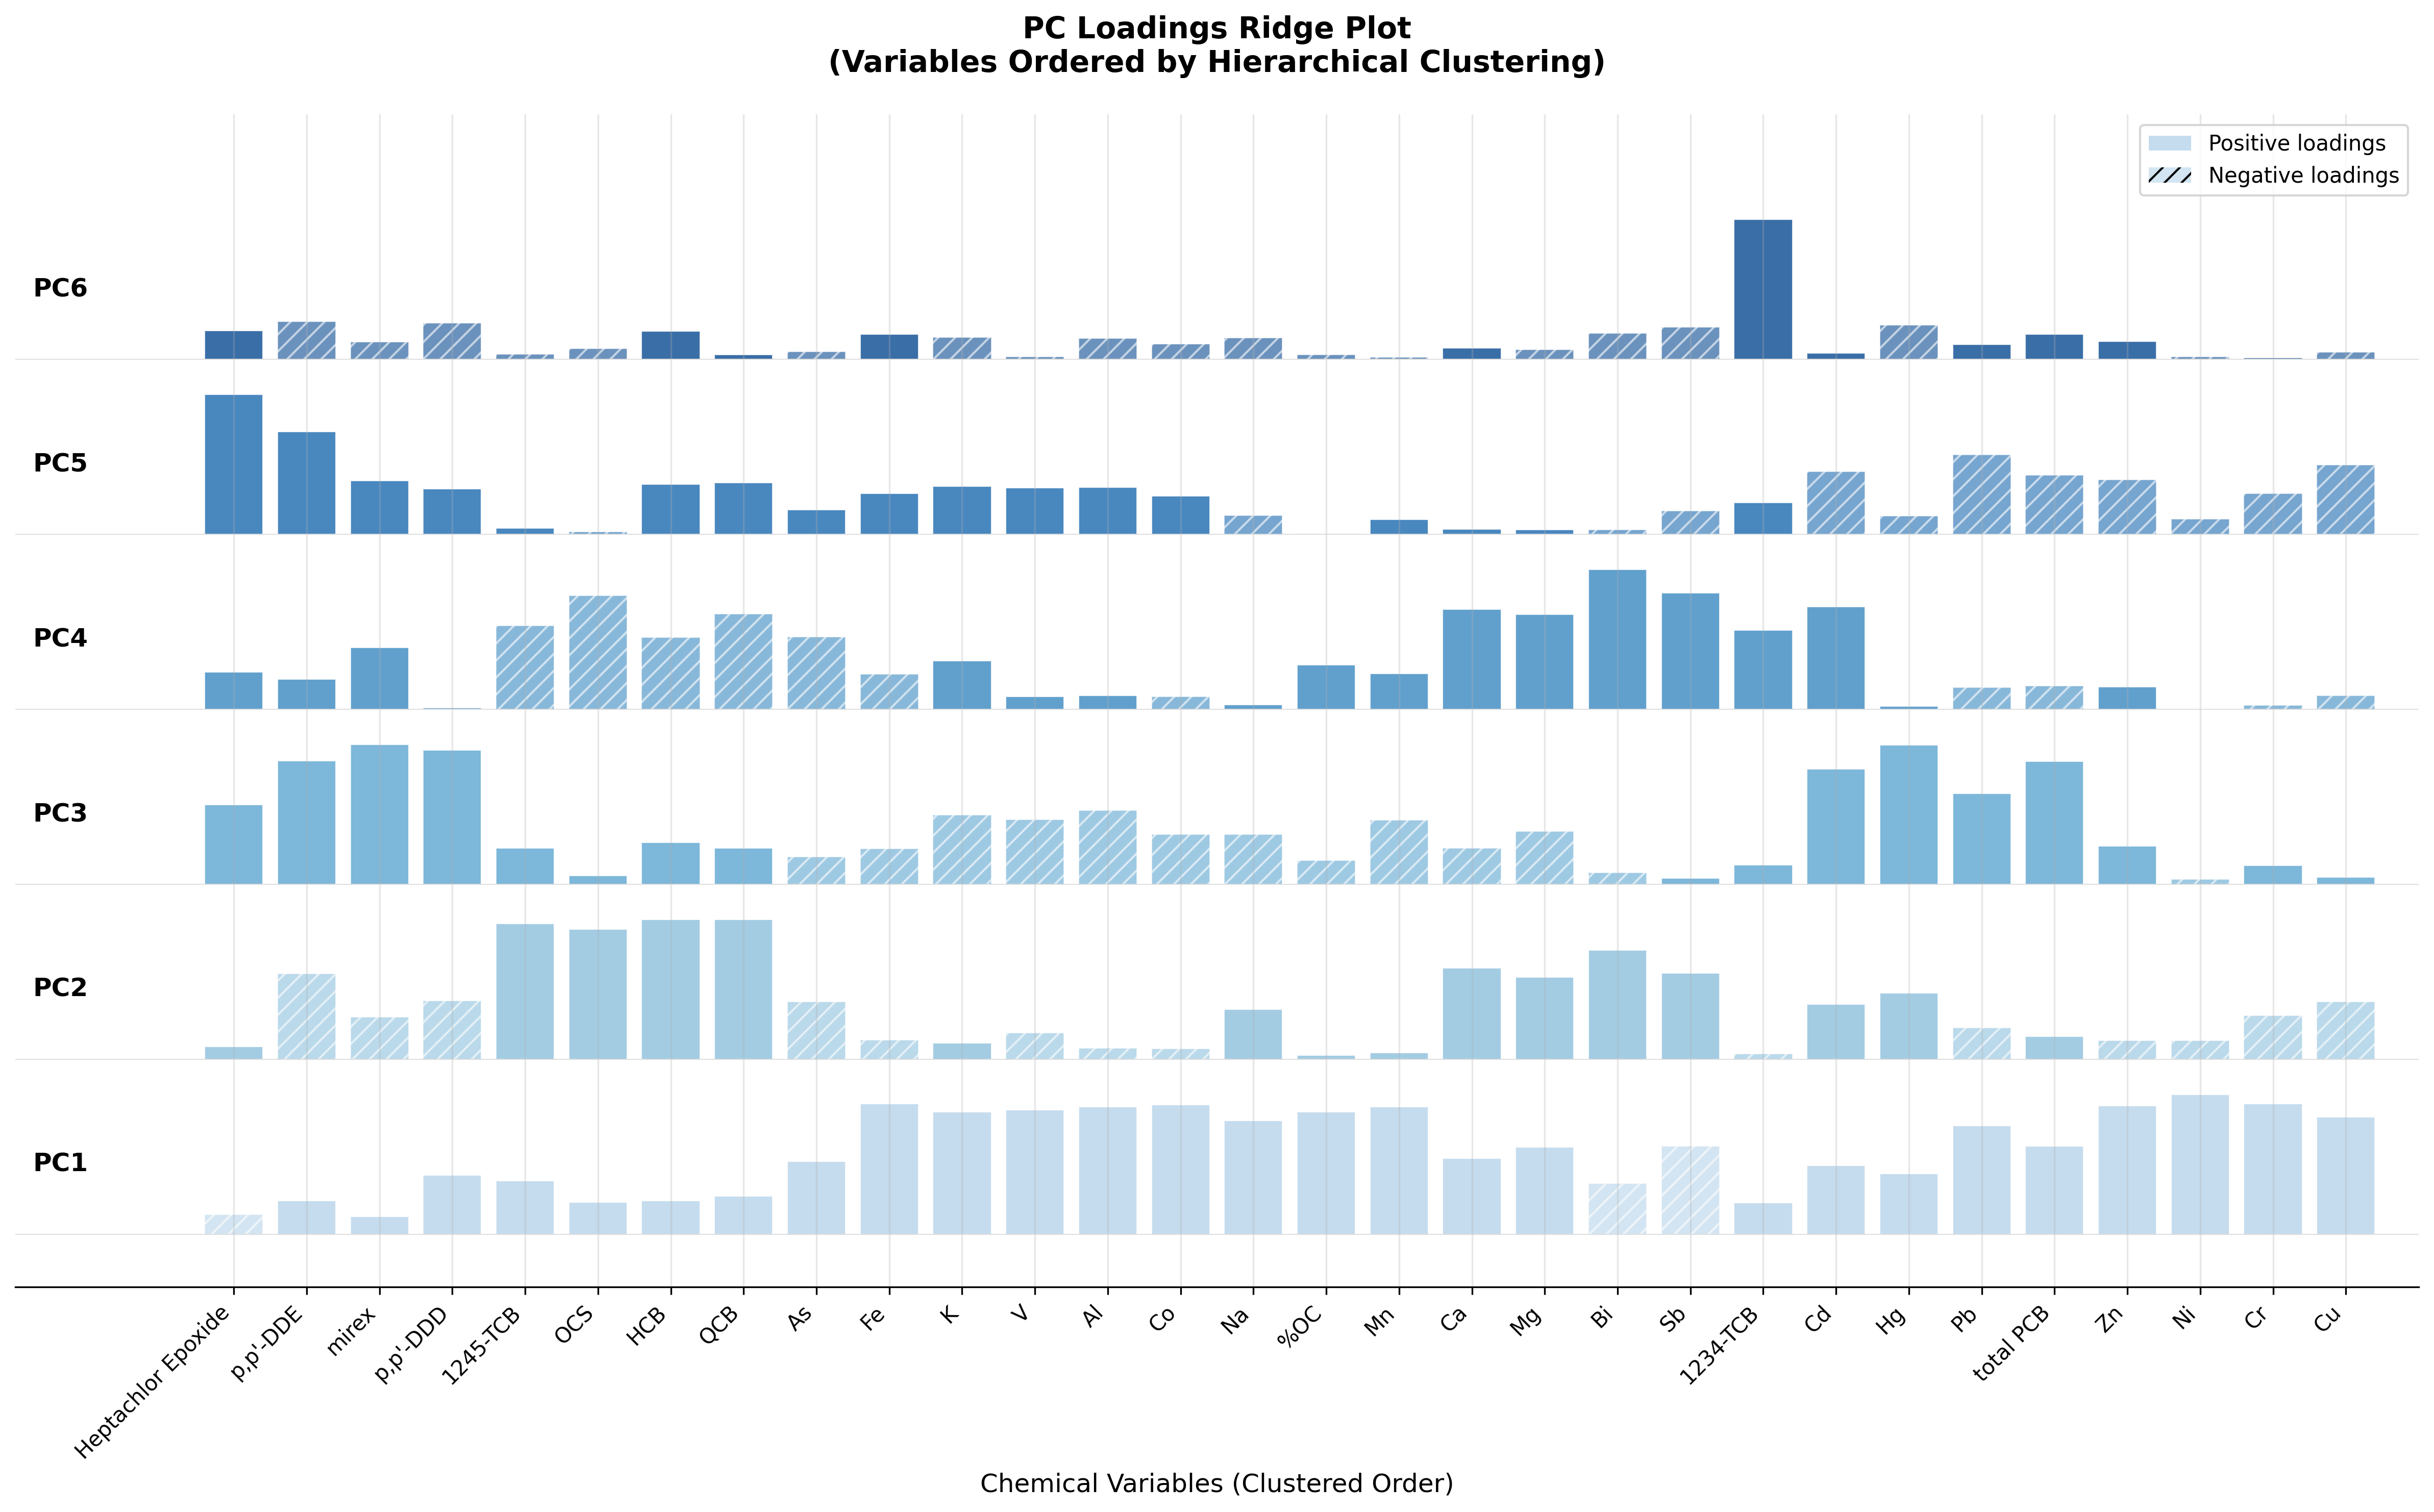
\includegraphics[width=0.9\textwidth]{../results/figures/01_contamination_assessment/figure2_pc_loadings_ridge.png}
    \caption{PC Loadings Ridge}
    \label{fig:01_pc_loadings_ridge}
\end{figure}

\begin{figure}[htbp]
    \centering
    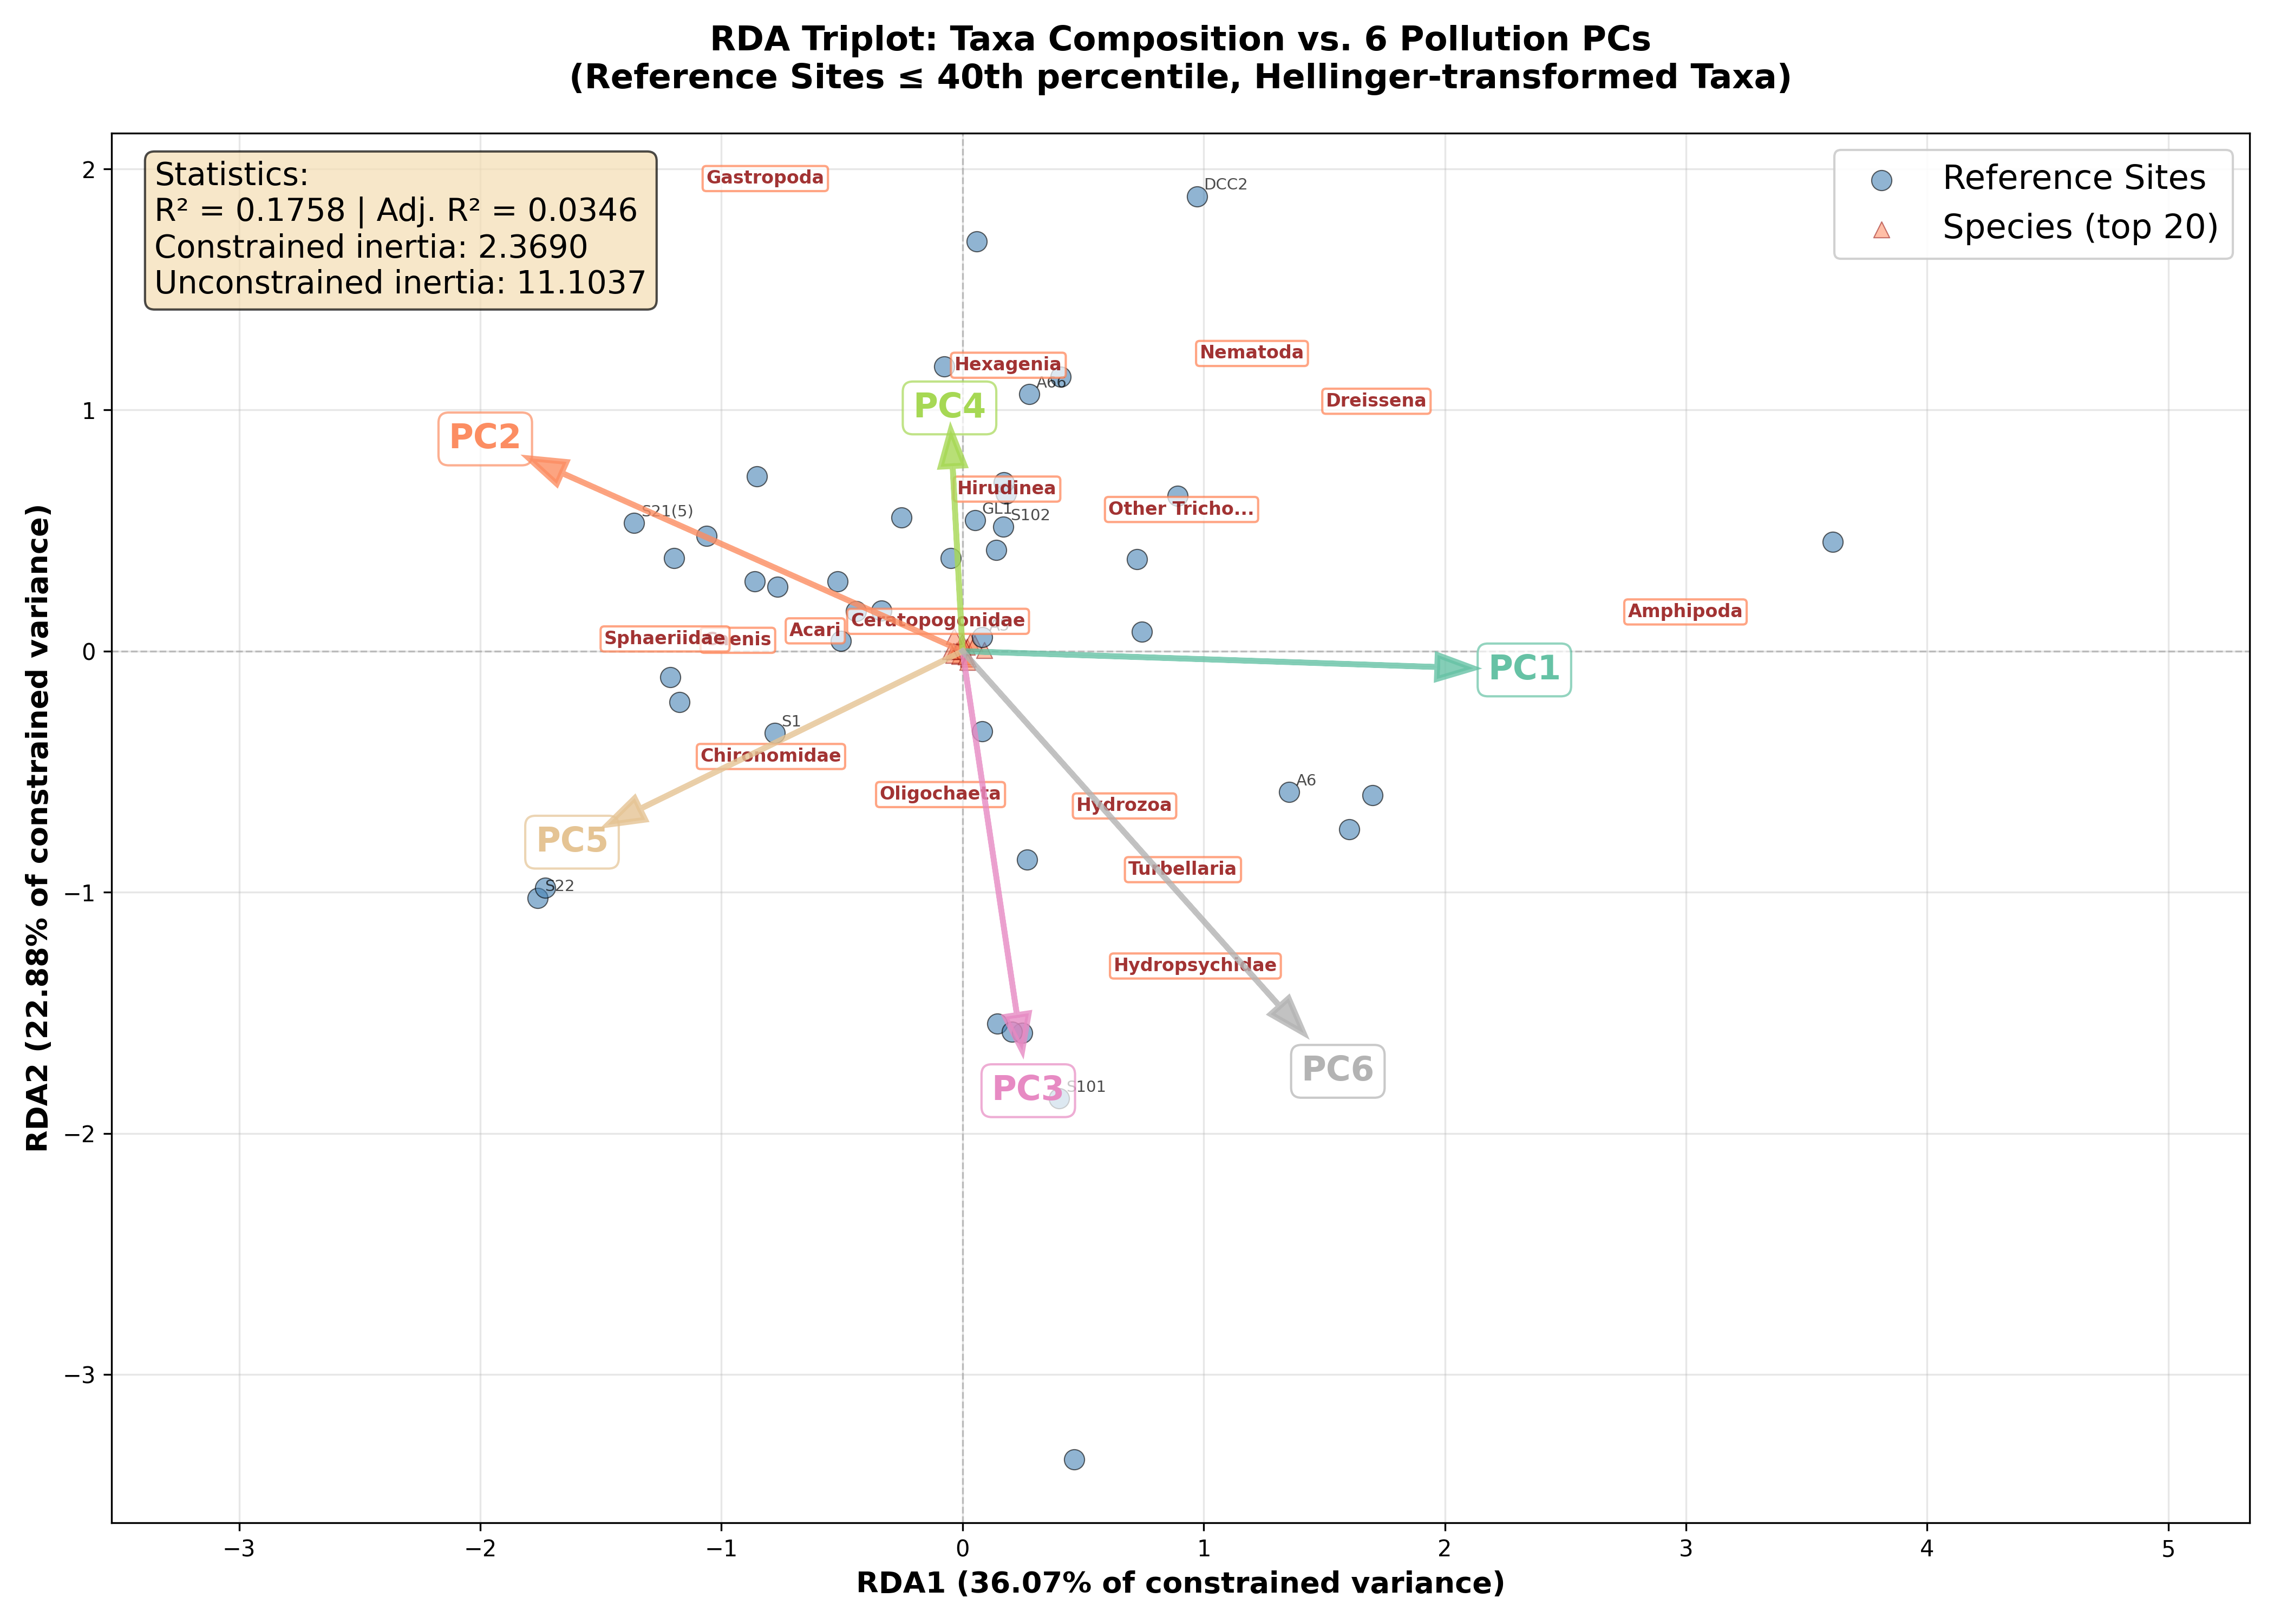
\includegraphics[width=0.9\textwidth]{../results/figures/01_contamination_assessment/RDA_triplot_pollution_species.png}
    \caption{RDA Triplot Pollution Species}
    \label{fig:01_rda_triplot_pollution_species}
\end{figure}


\chapter{Taxa Assemblage in Reference Sites}


\begin{figure}[htbp]
    \centering
    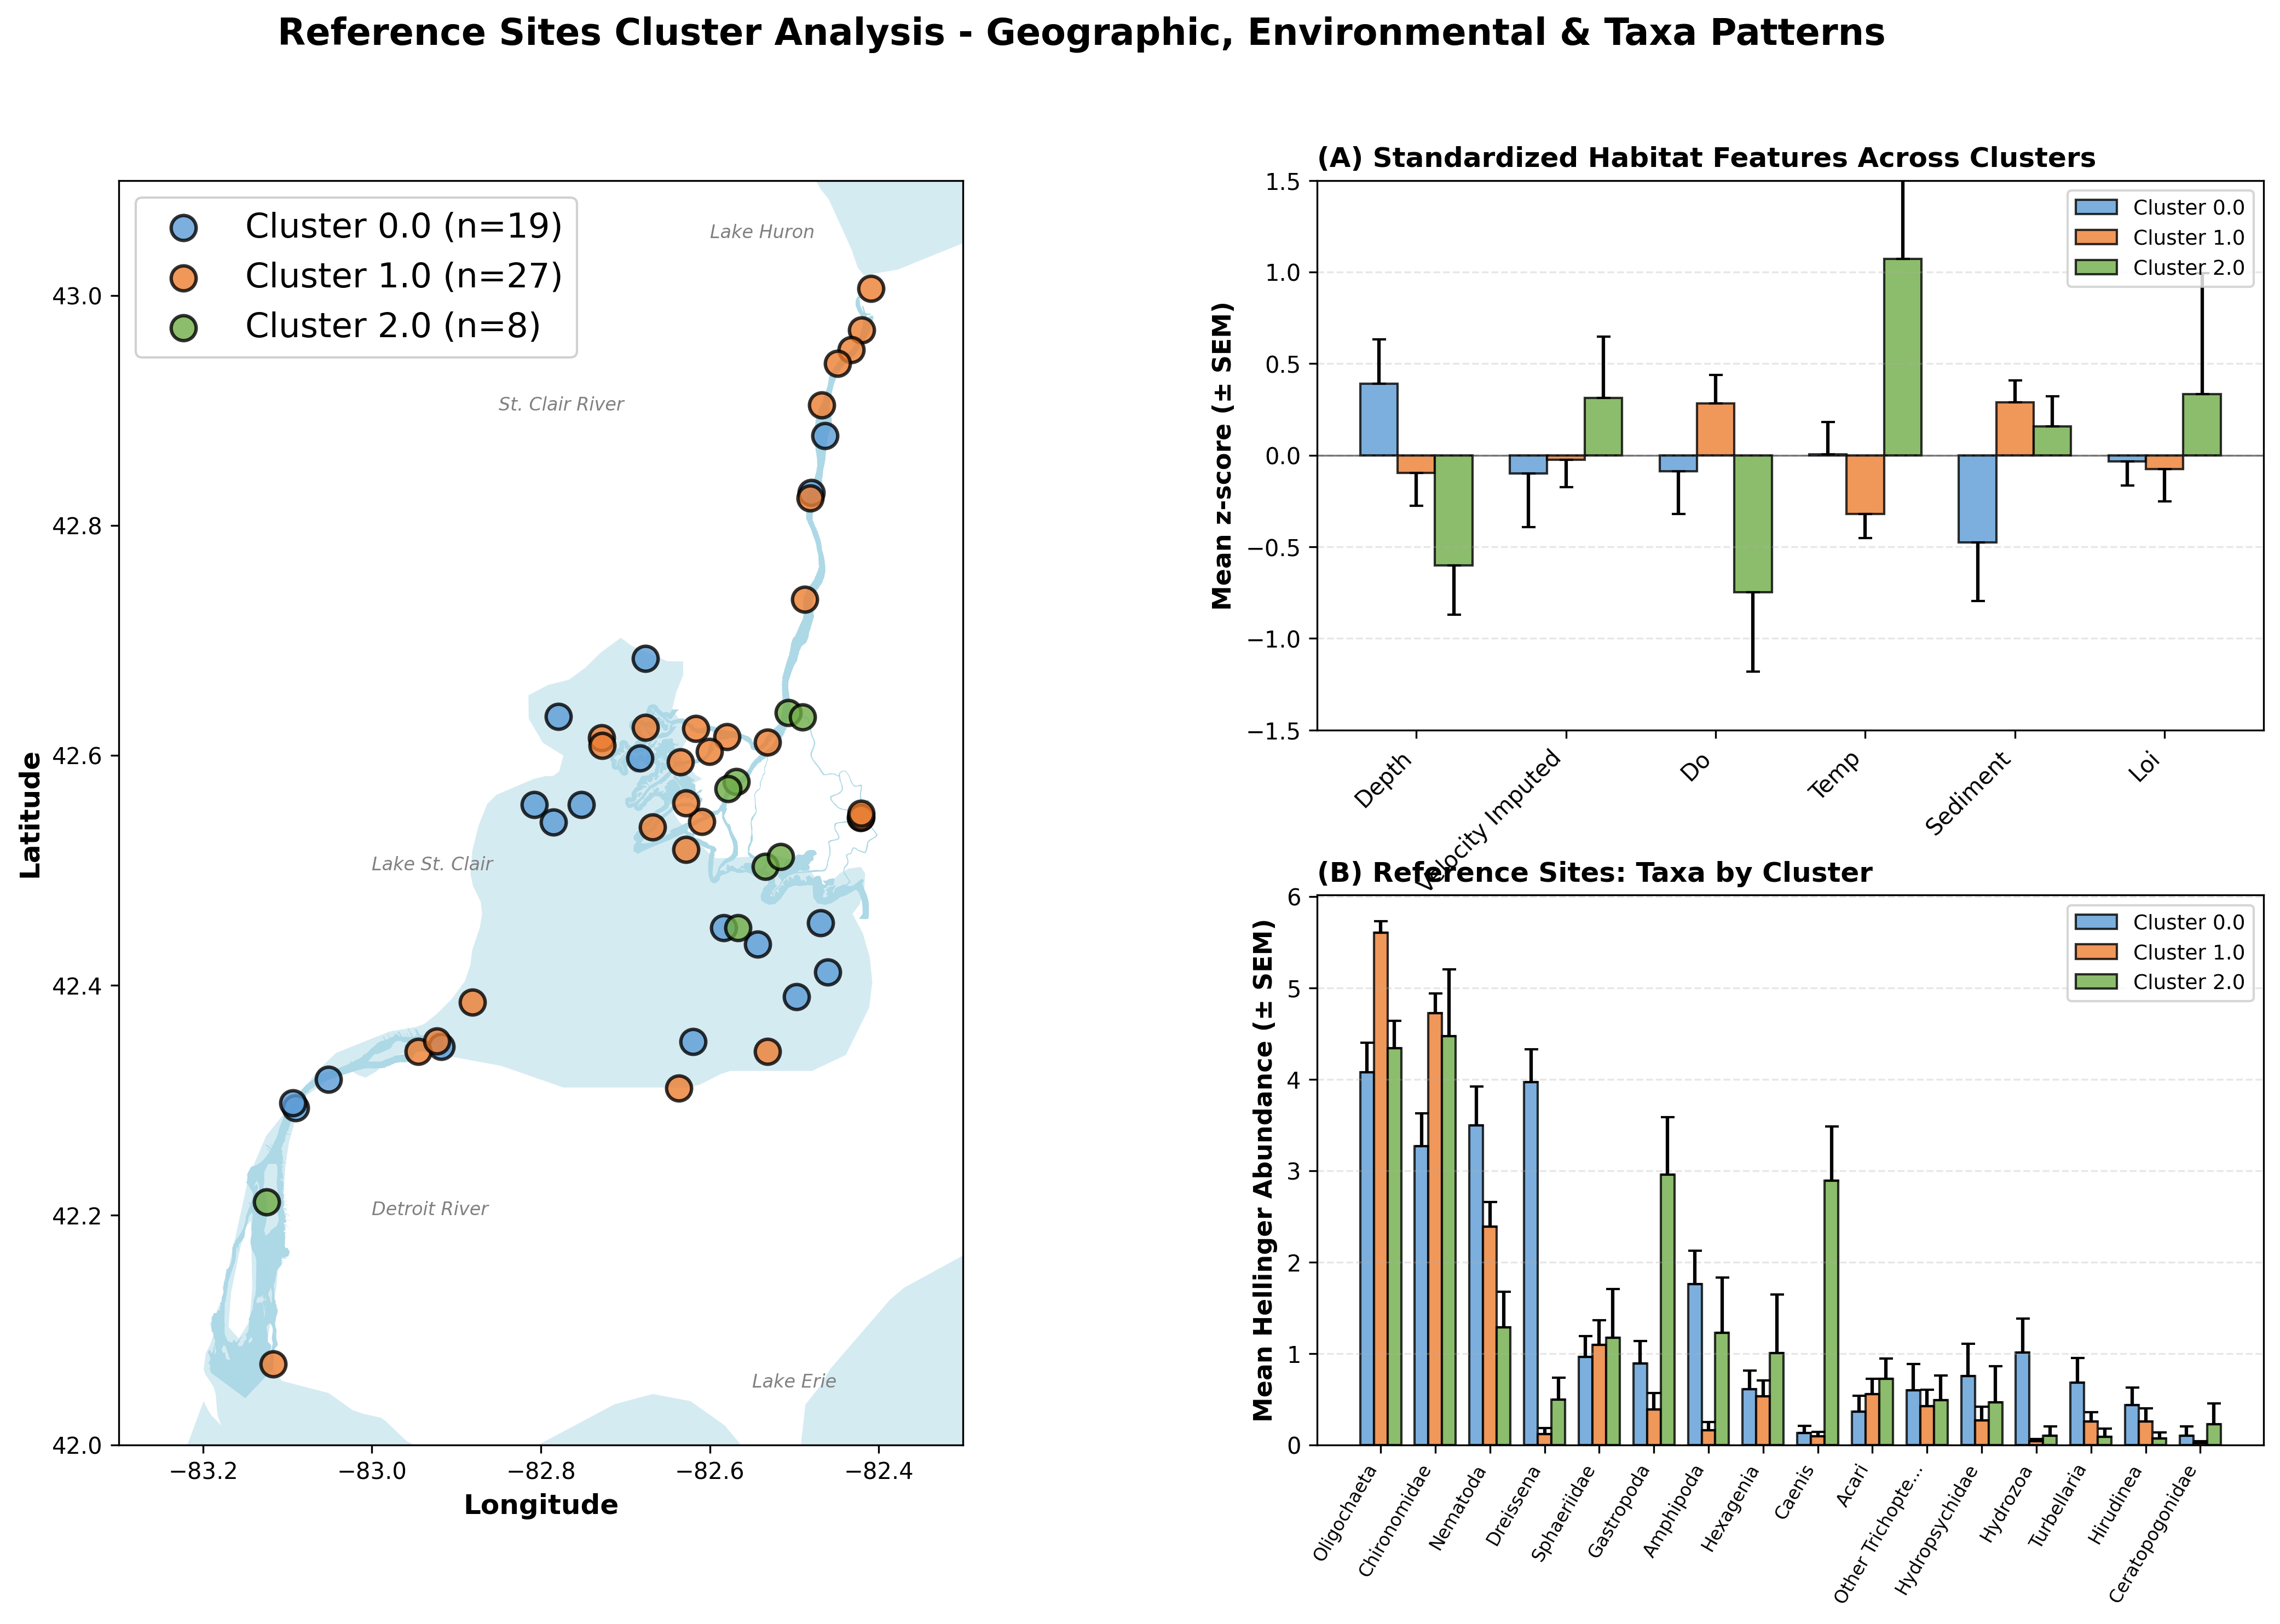
\includegraphics[width=0.9\textwidth]{../results/figures/02_taxa_assemblage_in_refs/figure2_cluster_visualization.png}
    \caption{Cluster Visualization}
    \label{fig:02_cluster_visualization}
\end{figure}

\begin{figure}[htbp]
    \centering
    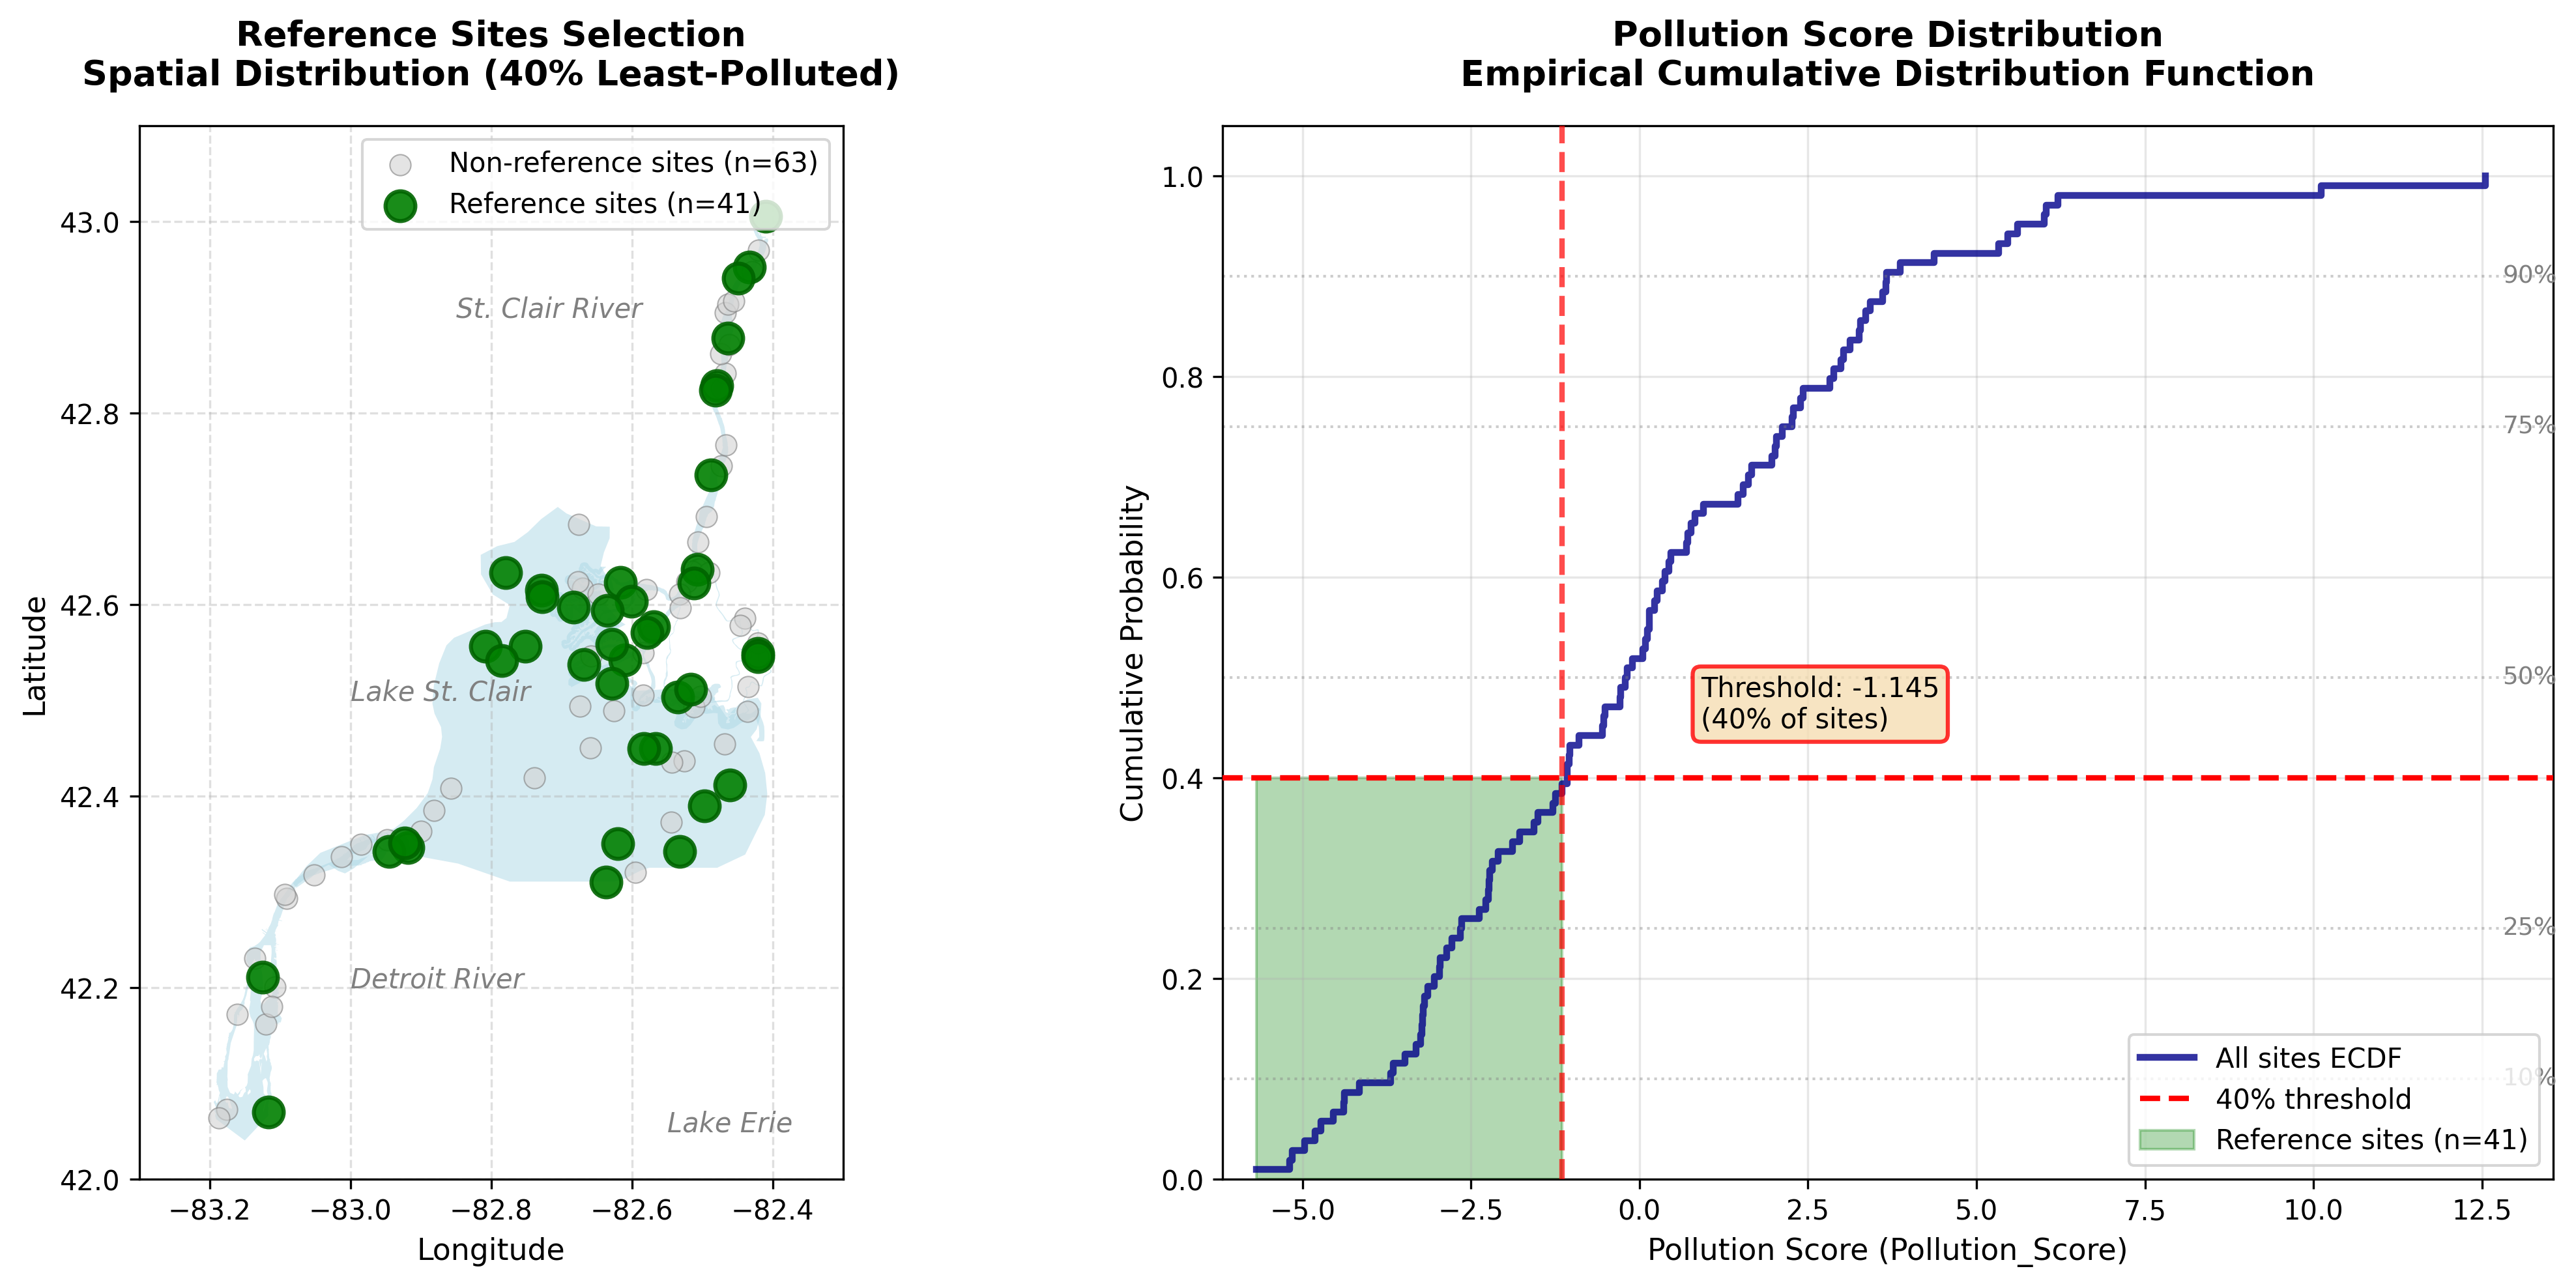
\includegraphics[width=0.9\textwidth]{../results/figures/02_taxa_assemblage_in_refs/figure2_reference_selection.png}
    \caption{Reference Selection}
    \label{fig:02_reference_selection}
\end{figure}

% \begin{figure}[htbp]
%     \centering
%     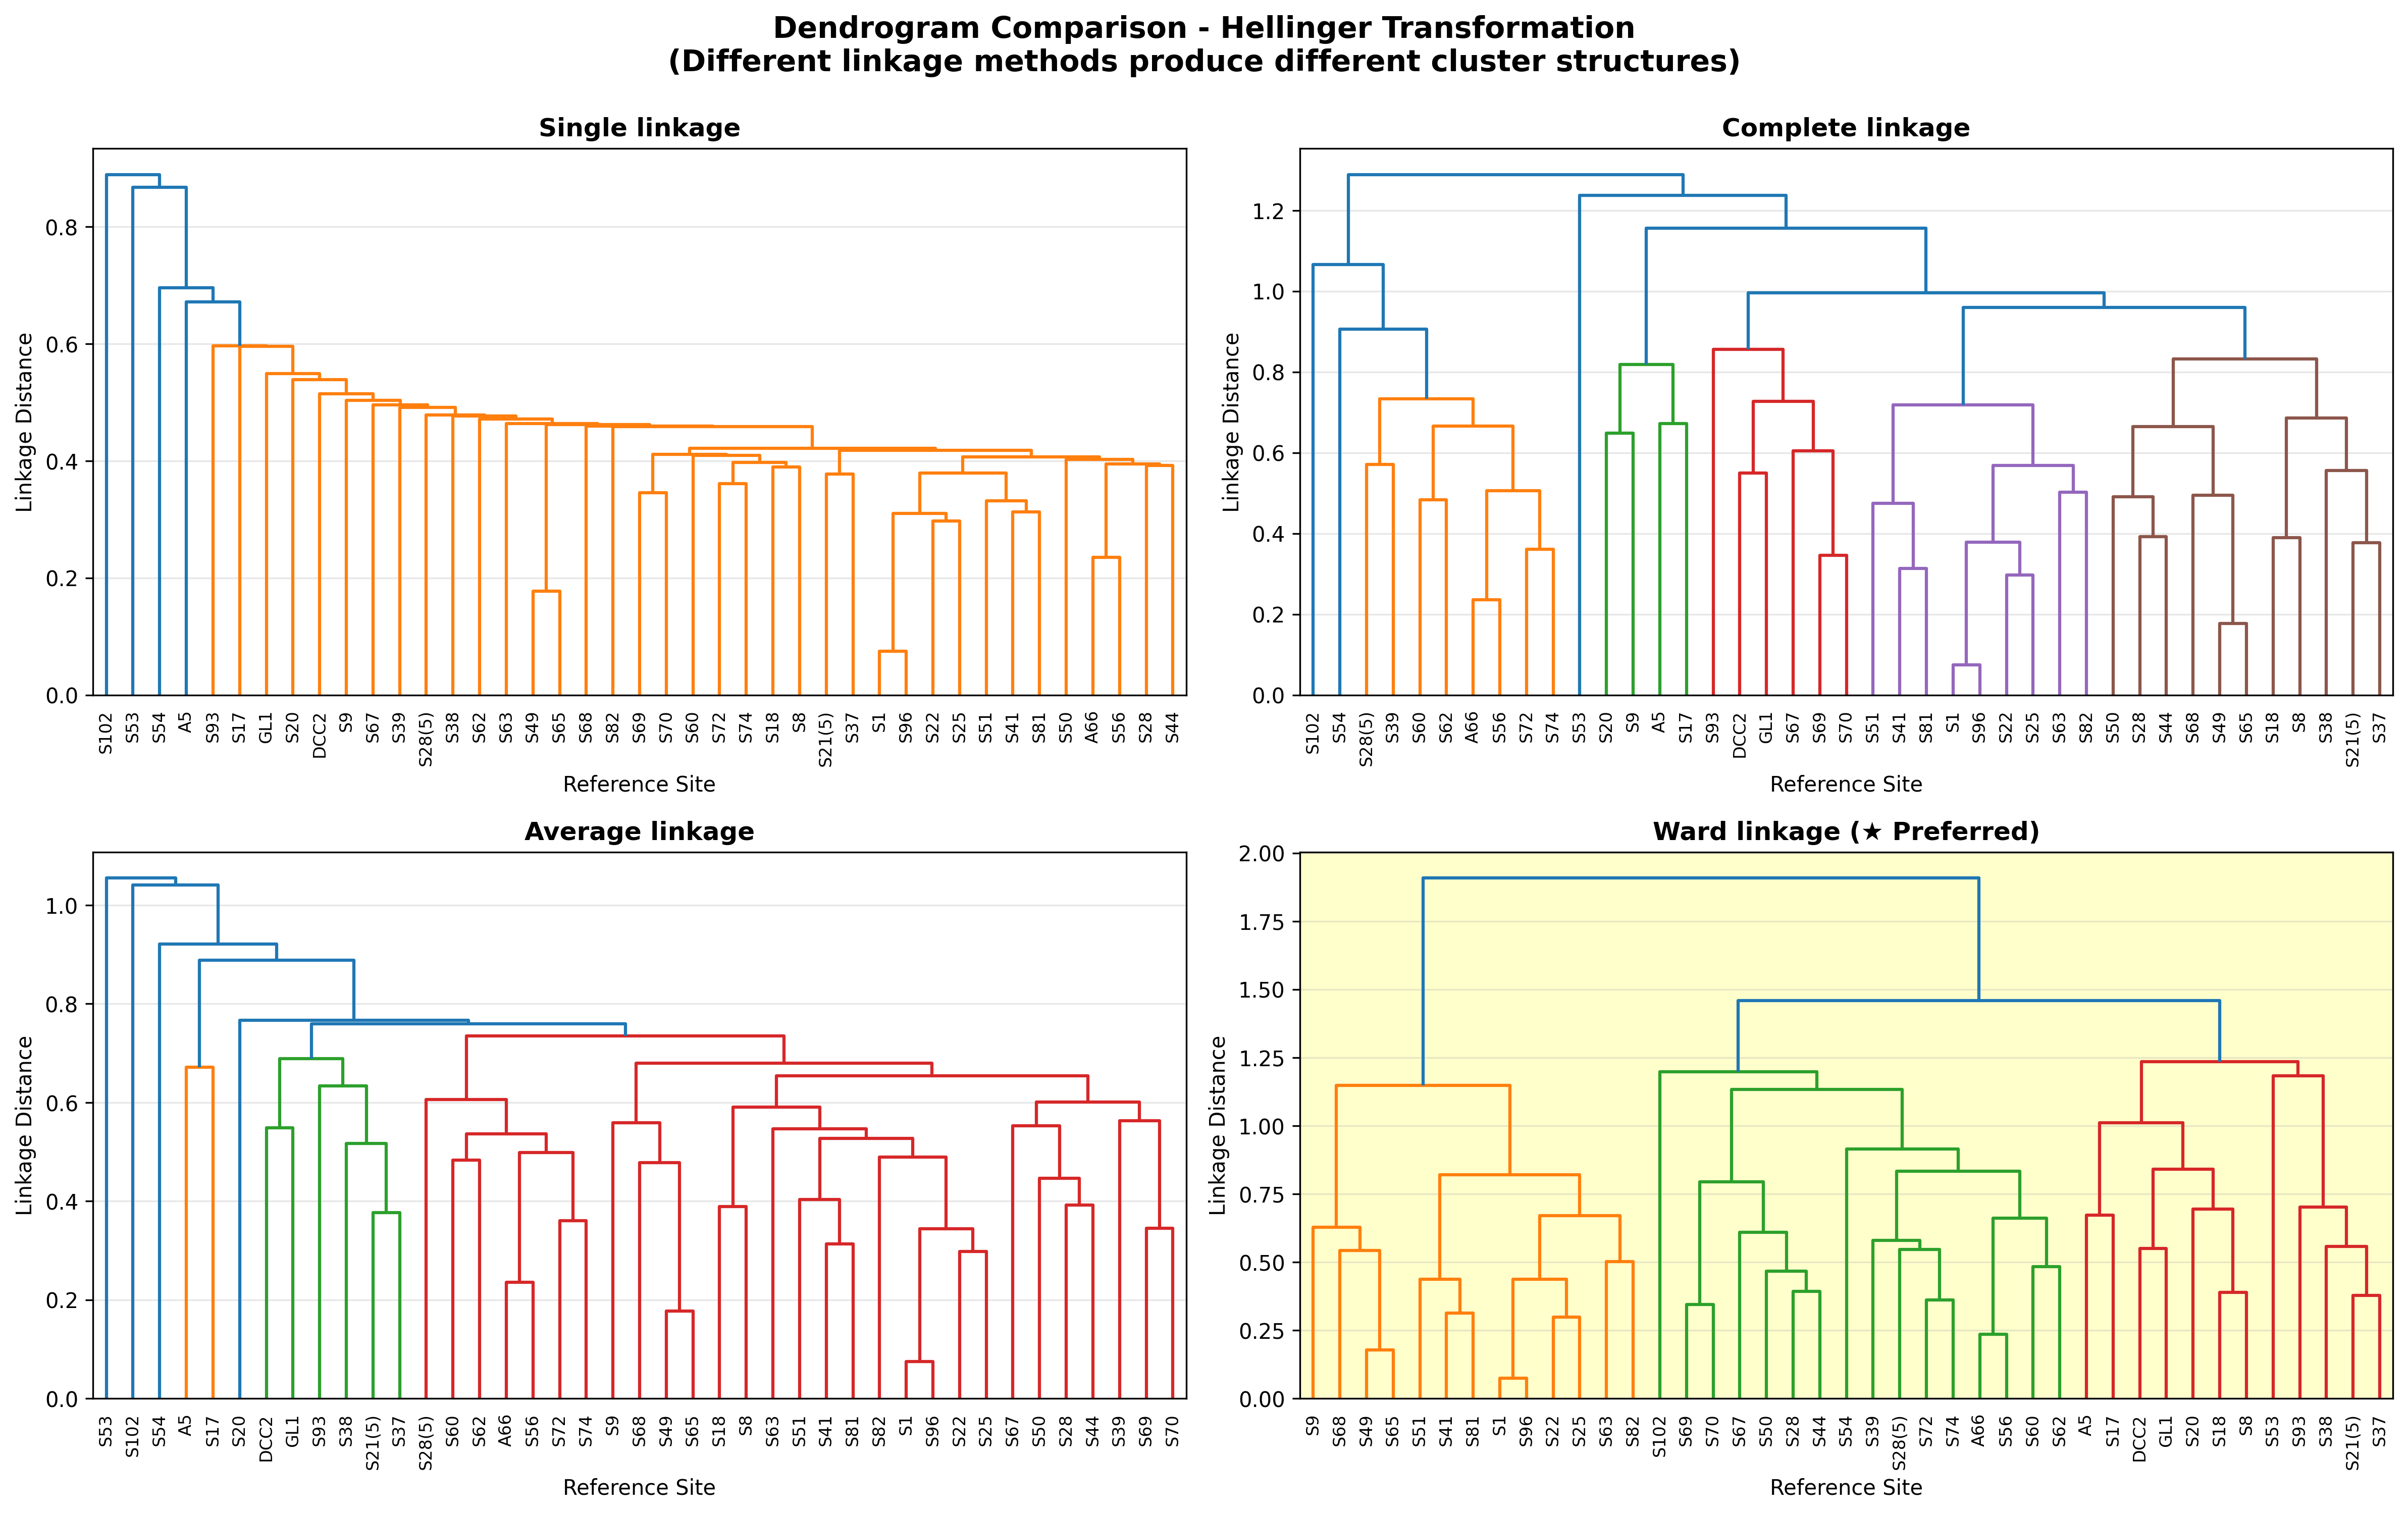
\includegraphics[width=0.9\textwidth]{../results/figures/02_taxa_assemblage_in_refs/figure3_dendrogram_comparison.png}
%     \caption{Dendrogram Comparison}
%     \label{fig:02_dendrogram_comparison}
% \end{figure}

% \begin{figure}[htbp]
%     \centering
%     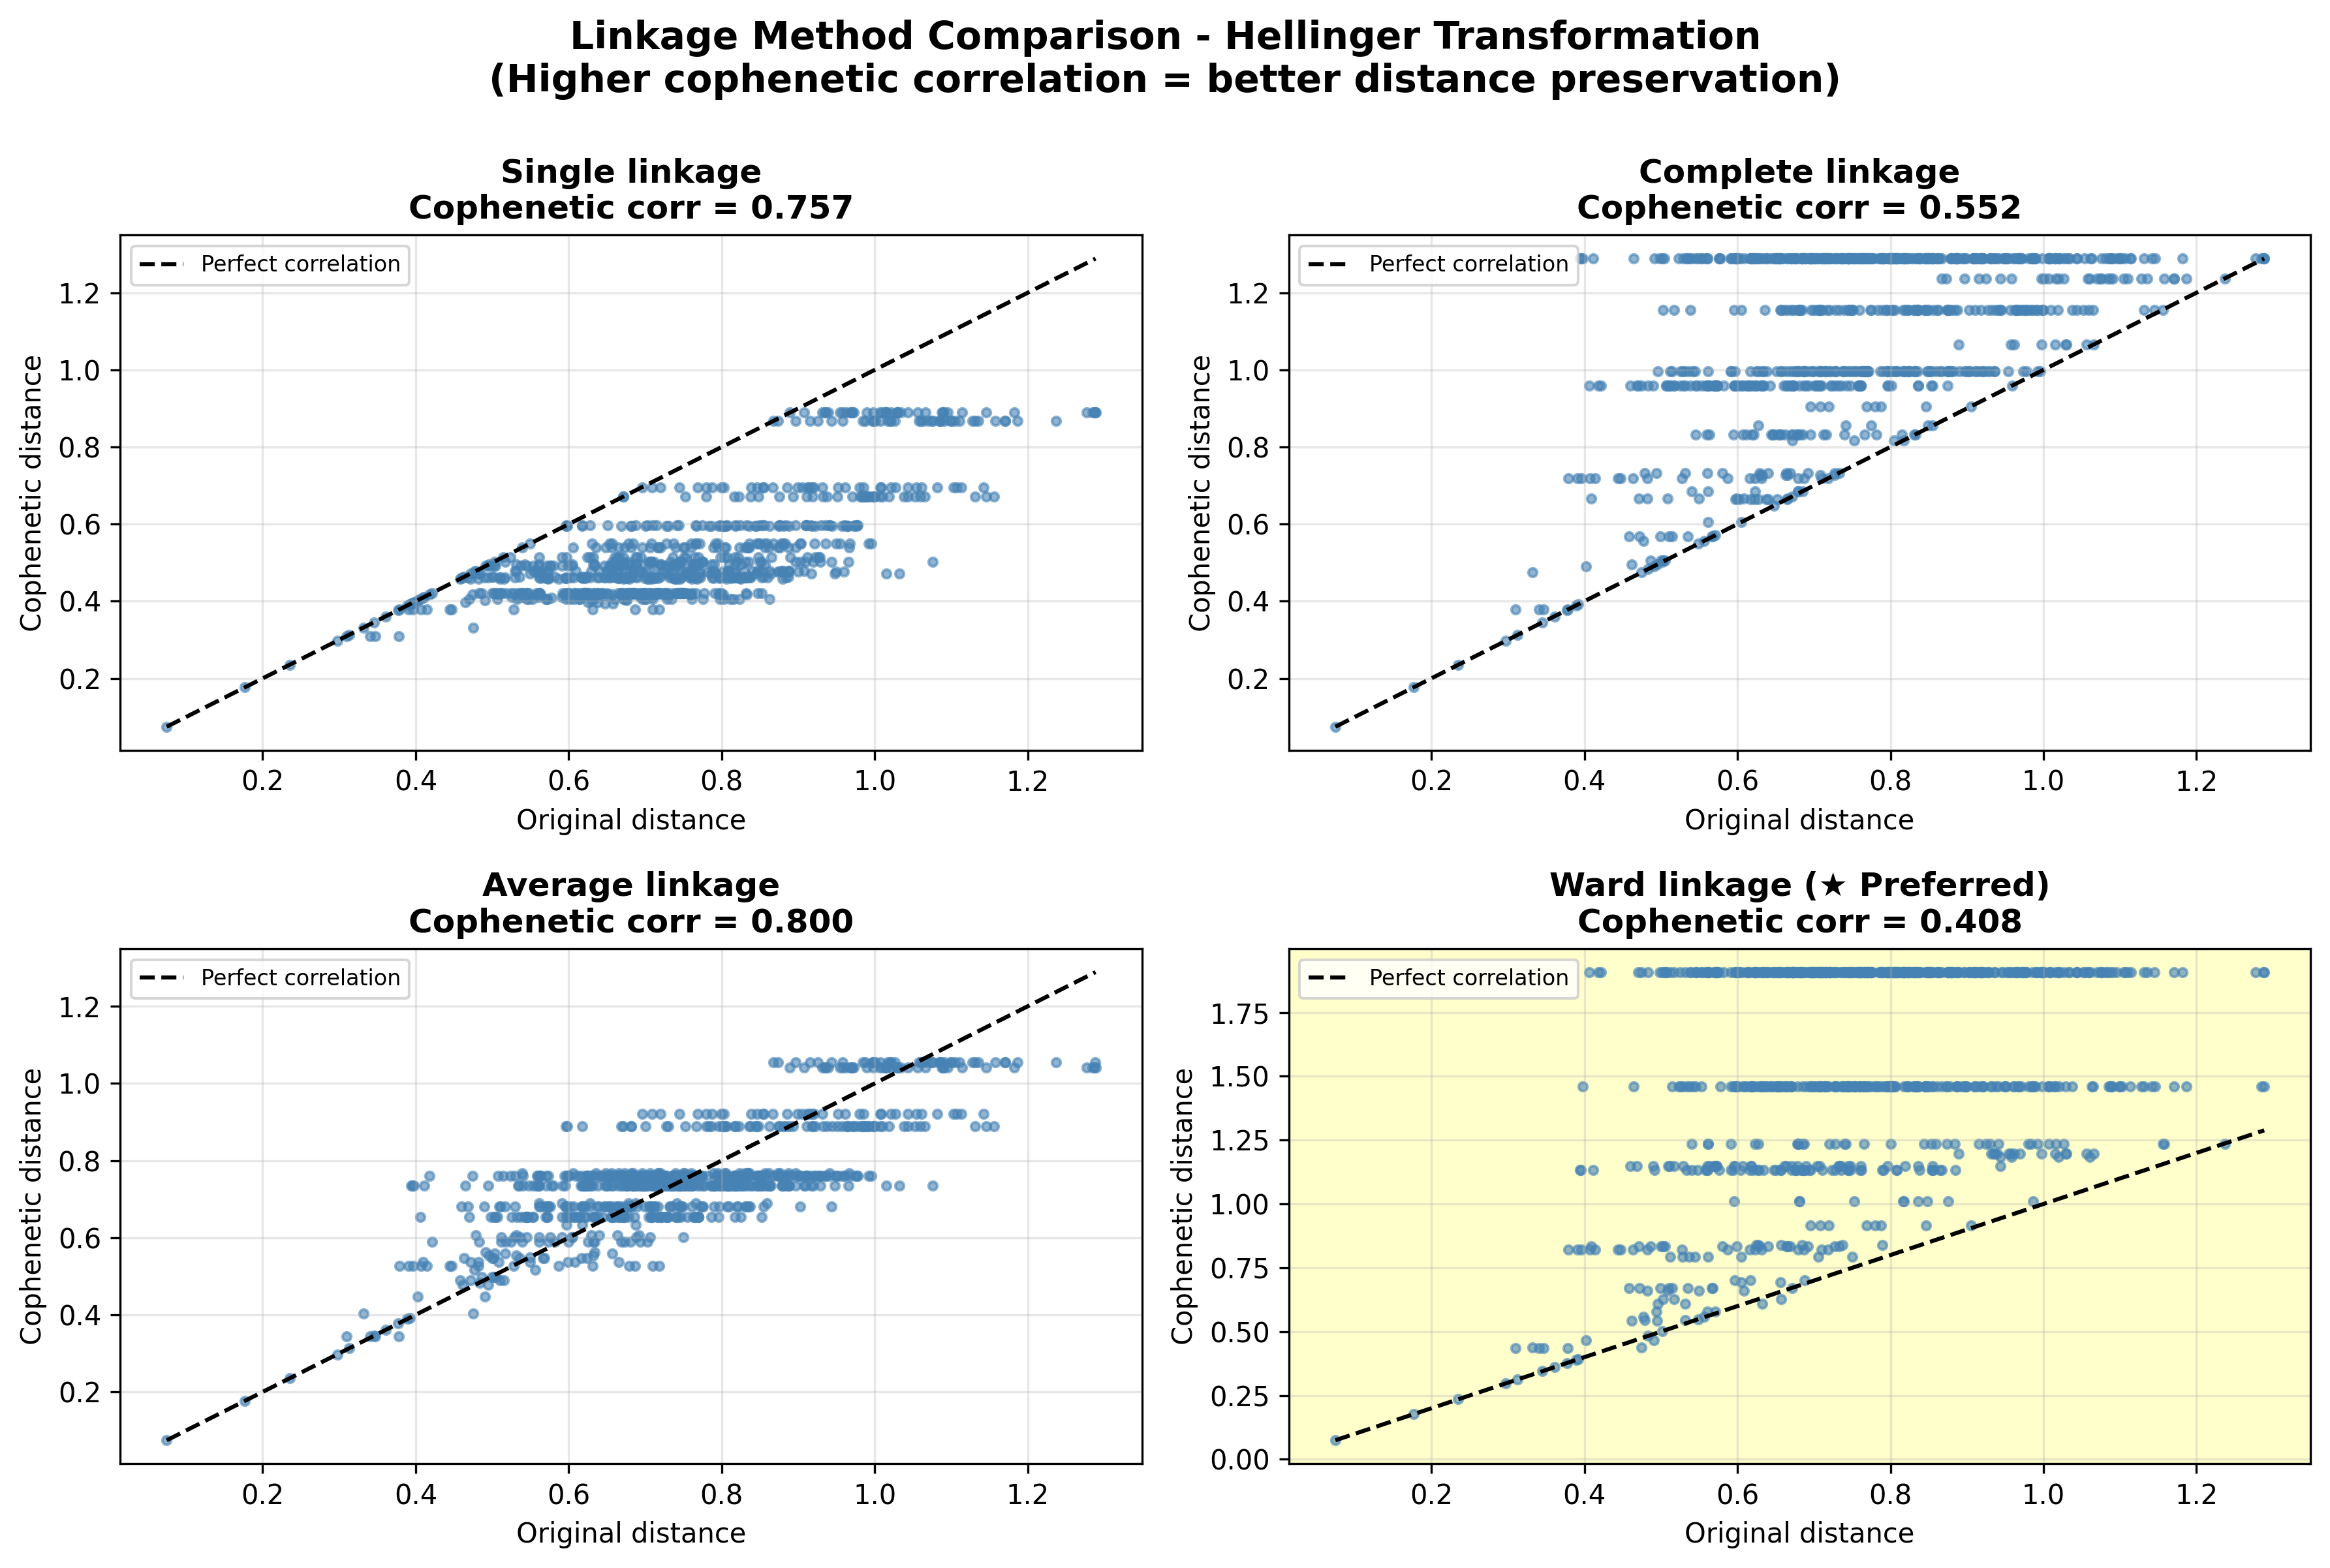
\includegraphics[width=0.9\textwidth]{../results/figures/02_taxa_assemblage_in_refs/figure4_linkage_comparison.png}
%     \caption{Linkage Comparison}
%     \label{fig:02_linkage_comparison}
% \end{figure}

\begin{figure}[htbp]
    \centering
    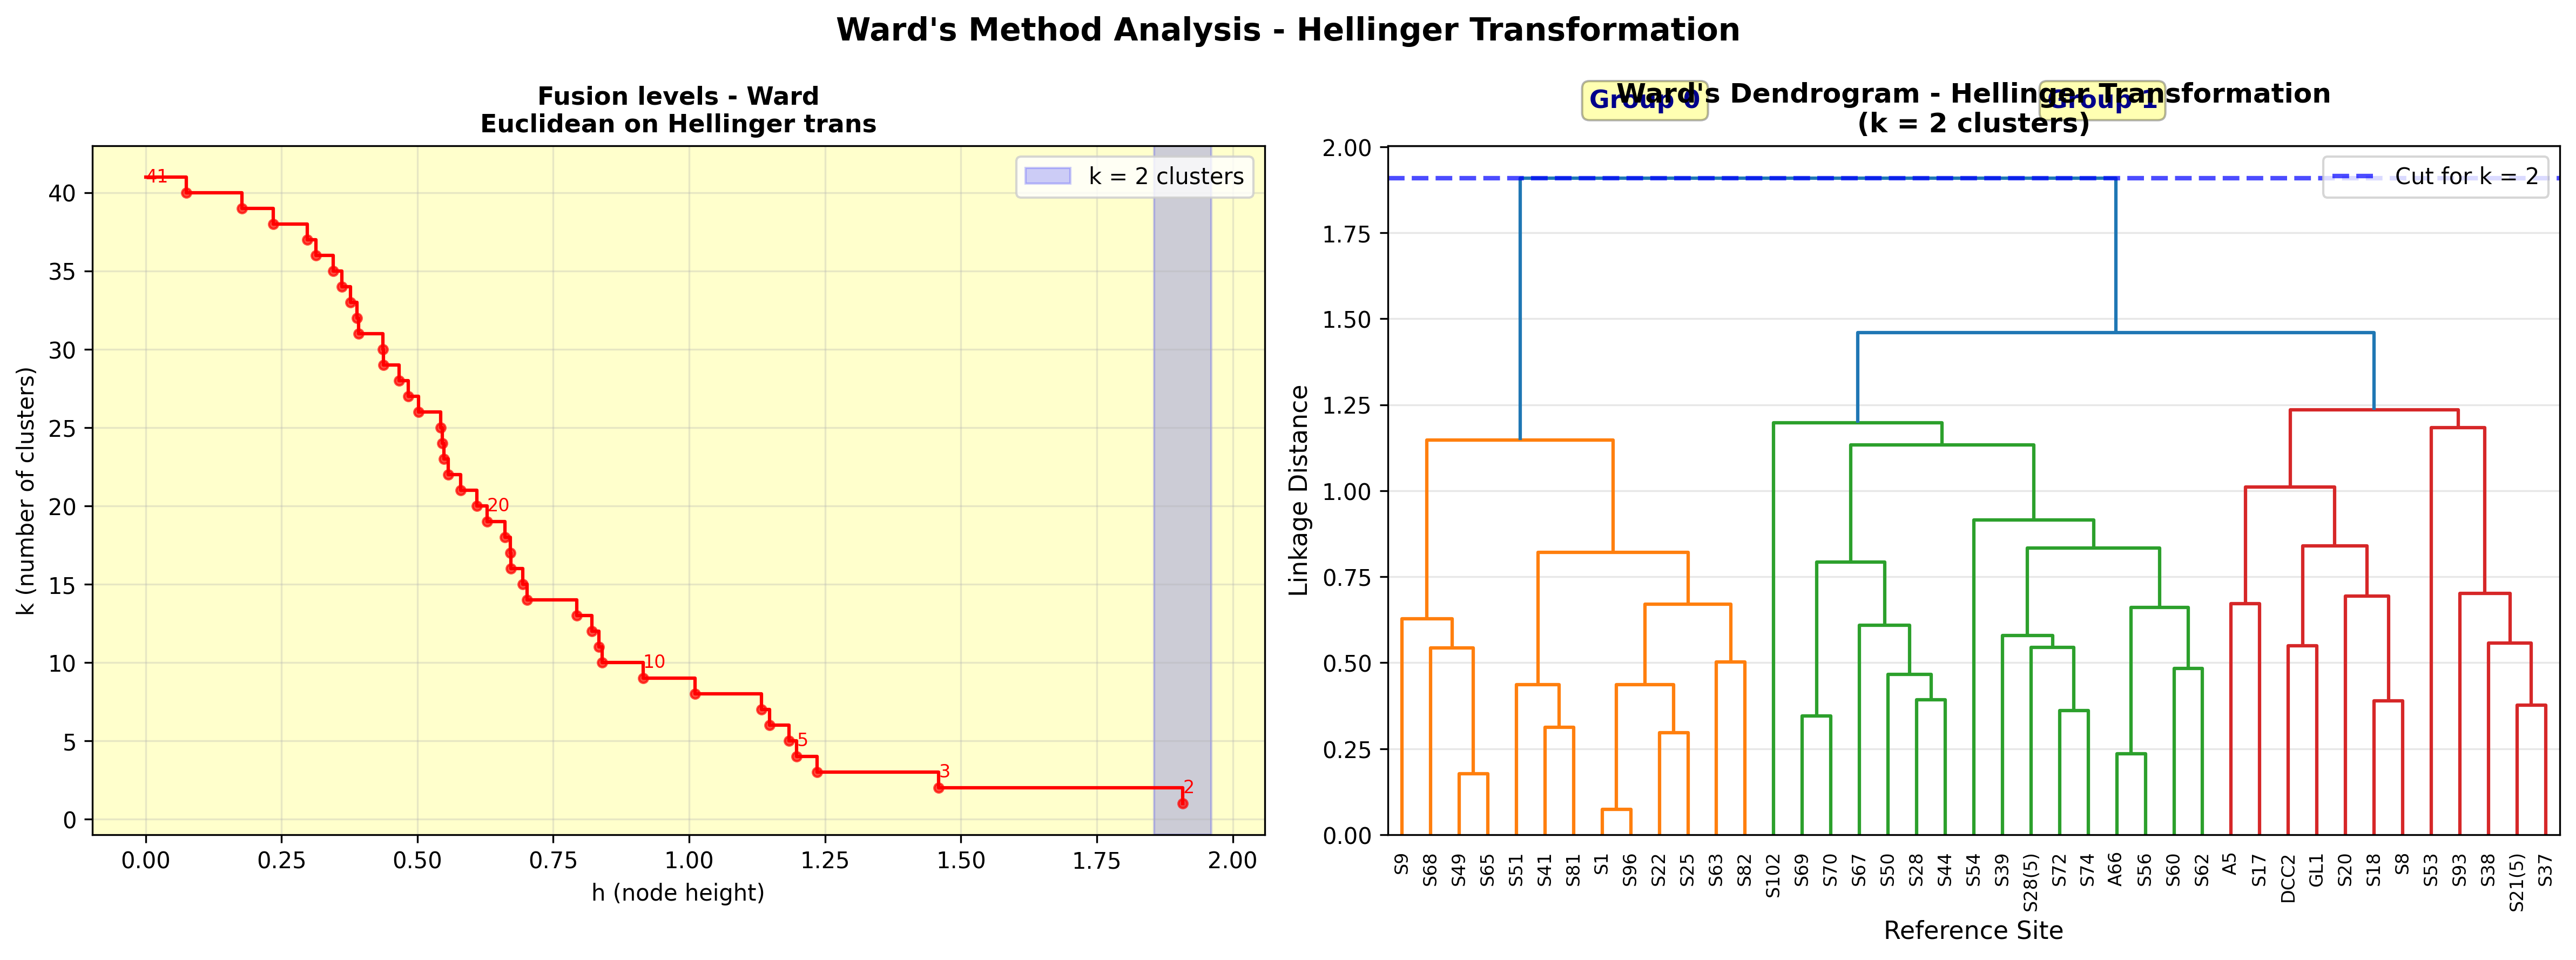
\includegraphics[width=0.9\textwidth]{../results/figures/02_taxa_assemblage_in_refs/figure5_ward_analysis.png}
    \caption{Ward Analysis}
    \label{fig:02_ward_analysis}
\end{figure}

\begin{figure}[htbp]
    \centering
    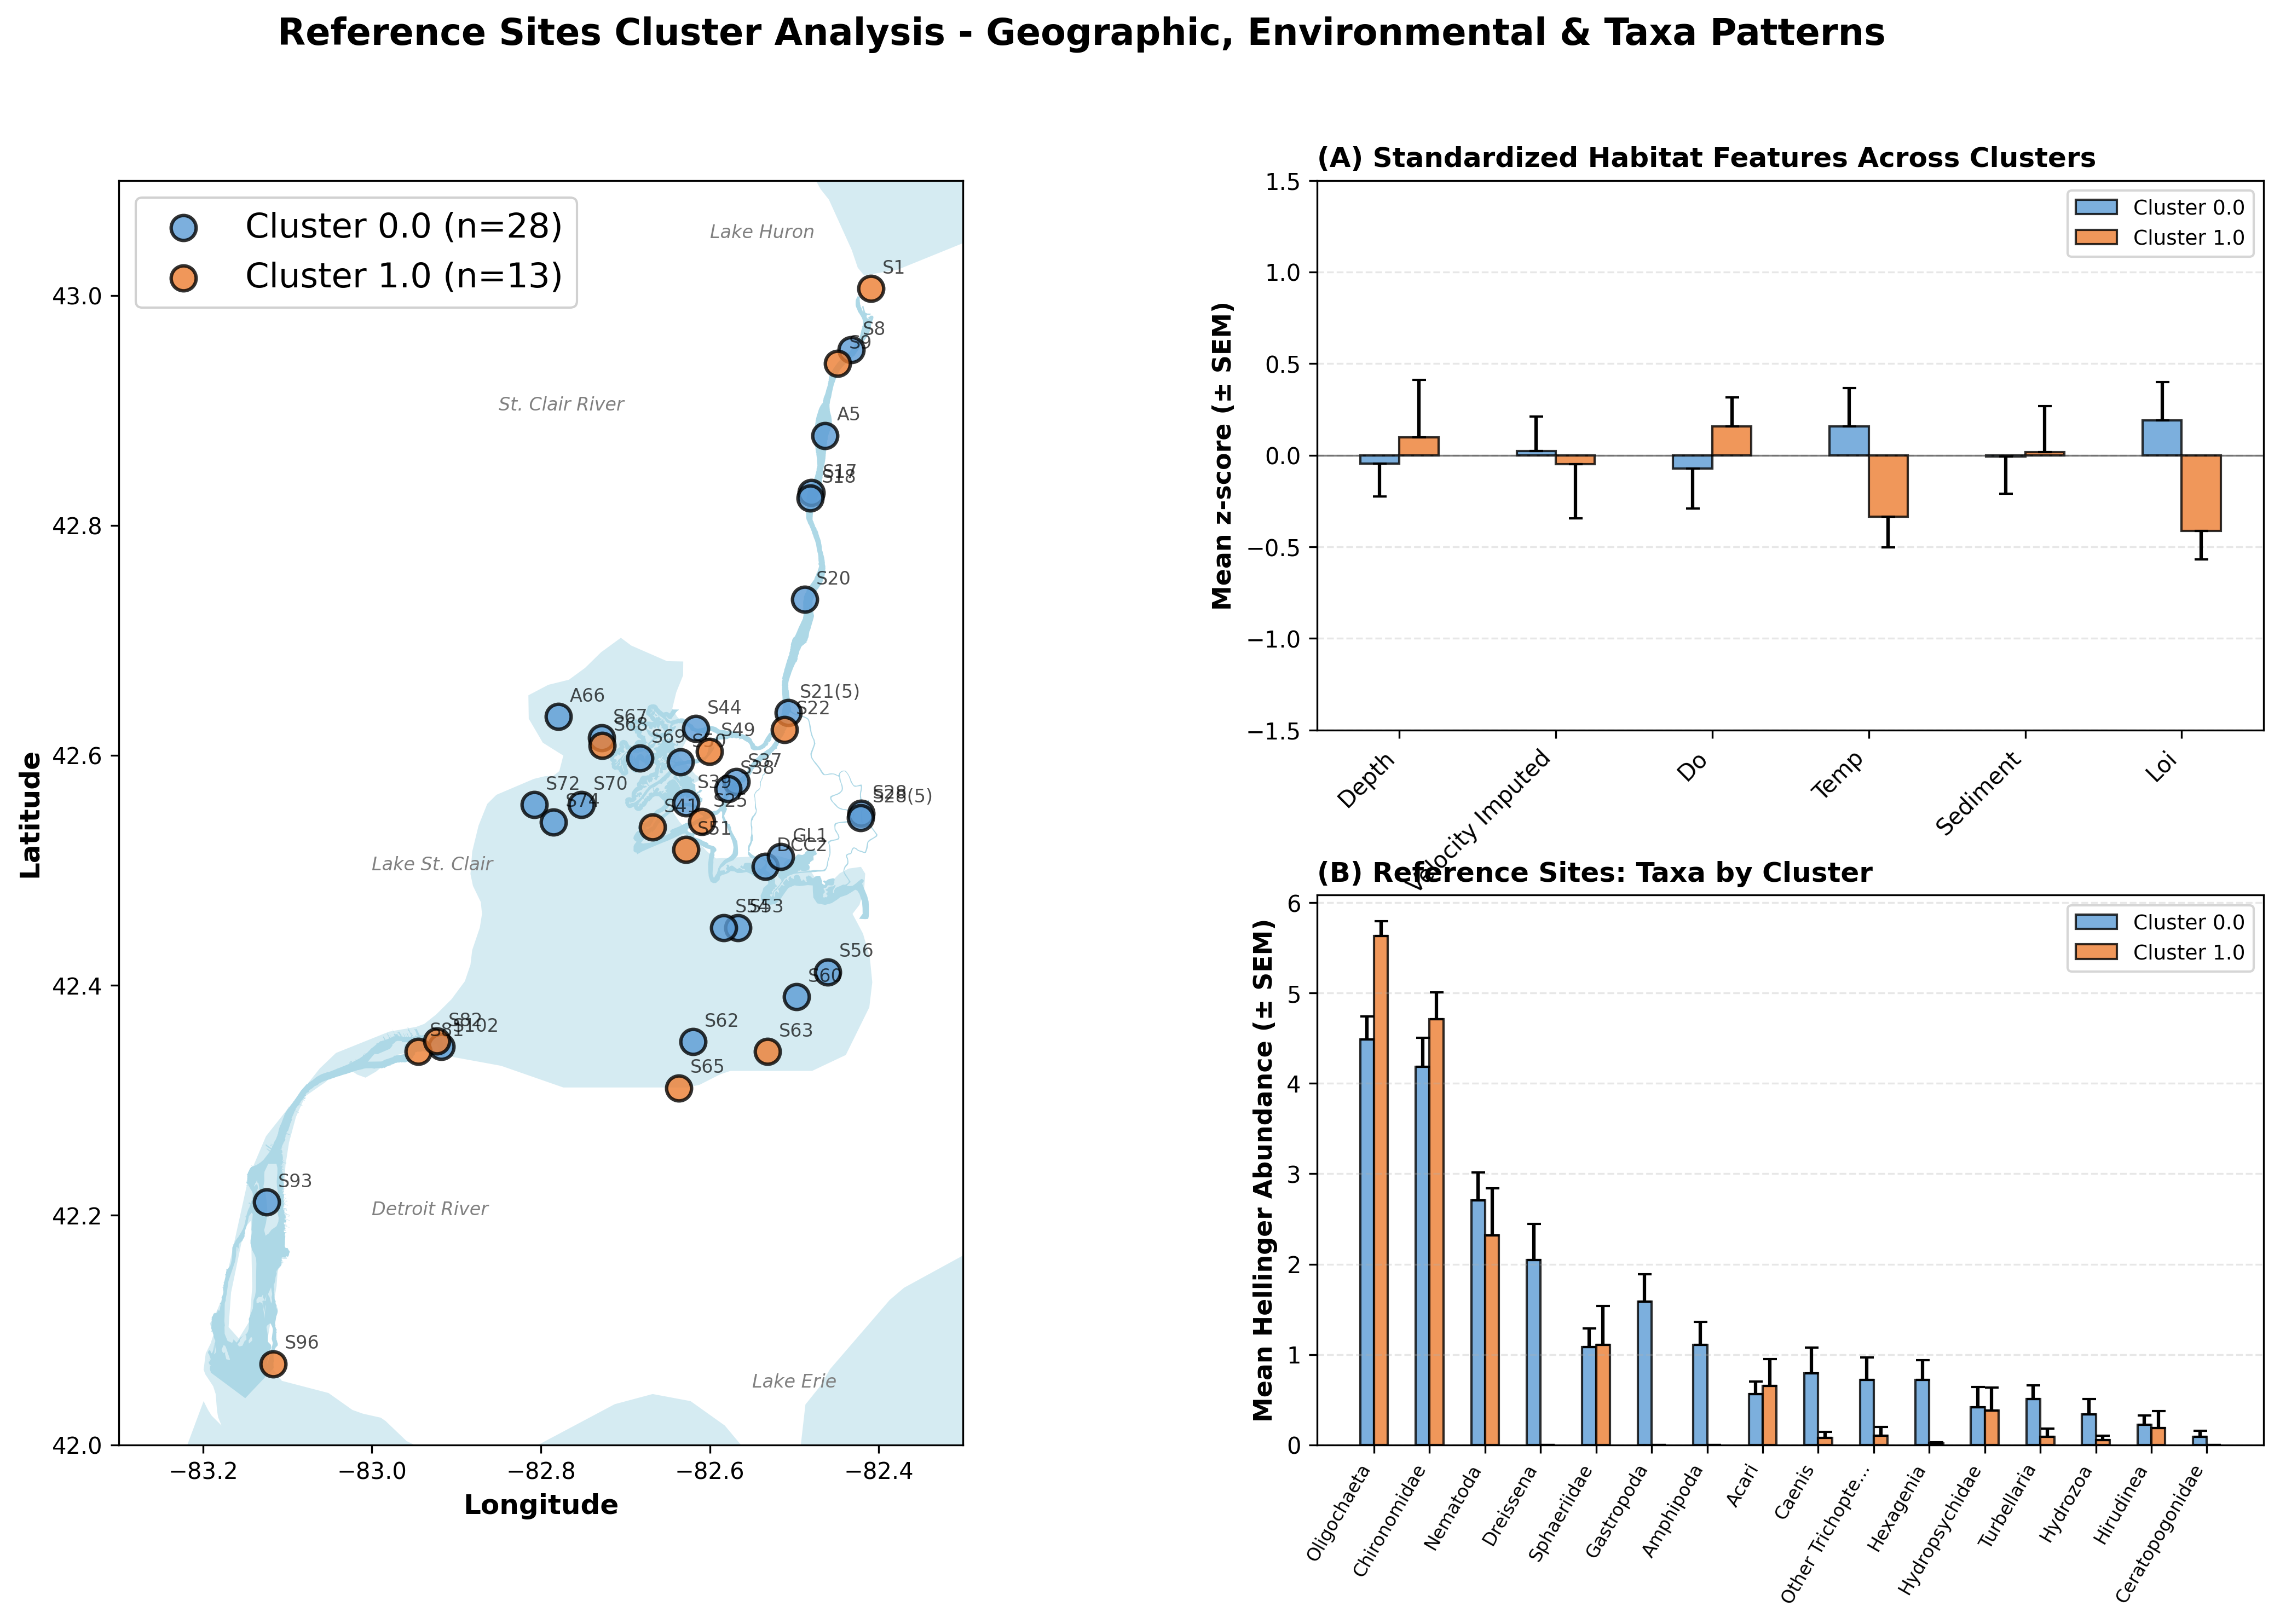
\includegraphics[width=0.9\textwidth]{../results/figures/02_taxa_assemblage_in_refs/figure6_cluster_visualization.png}
    \caption{Cluster Visualization Final}
    \label{fig:02_cluster_visualization_final}
\end{figure}



% =============================================================================
% Environmental Characteristics by Cluster
% =============================================================================
\begin{table}[htbp]
\centering
\footnotesize
\caption{Environmental Characteristics by Cluster (Reference Sites Only)}
\label{tab:02_env_characteristics}
\begin{tabular}{@{}lccc>{\centering\arraybackslash}p{1.5cm}@{}}
\toprule
Variable & Cluster 0 & Cluster 1 & Cluster 2 & F-stat \\
\midrule
Depth (m) & 4.48 $\pm$ 2.74 & 3.50 $\pm$ 2.48 & 2.06 $\pm$ 2.04 & 2.62 \\
Velocity (m/sec) & 0.09 $\pm$ 0.13 & 0.12 $\pm$ 0.09 & 0.16 $\pm$ 0.11 & 1.20 \\
DO Bottom (mg/L) & 9.44 $\pm$ 0.96 & 9.77 $\pm$ 0.73 & 8.83 $\pm$ 1.12 & 3.68* \\
Temperature (\textdegree C) & 20.64 $\pm$ 1.38 & 19.90 $\pm$ 1.27 & 22.47 $\pm$ 2.90 & 7.90** \\
MPS (Phi) & 0.85 $\pm$ 1.34 & 1.50 $\pm$ 0.60 & 1.38 $\pm$ 0.46 & 2.88. \\
LOI (\%) & 1.77 $\pm$ 0.68 & 1.75 $\pm$ 1.04 & 2.20 $\pm$ 2.14 & 0.49 \\
\midrule
Sample size (n) & 18 & 28 & 8 & \\
Environment Type & Fine Silt & Silt / Organic Rich & Coarse Gravel/Cobble & \\
\bottomrule
\end{tabular}
\begin{flushleft}
\footnotesize{Significance: *** p$<$0.001, ** p$<$0.01, * p$<$0.05, . p$<$0.1}
\end{flushleft}
\end{table}

% =============================================================================
% Top Taxa Abundance by Cluster
% =============================================================================
\begin{table}[htbp]
\centering
\small
\caption{Top Taxa Abundance by Cluster (Reference Sites Only)}
\label{tab:02_taxa_abundance}
\begin{tabular}{@{}lccc>{\centering\arraybackslash}p{1.6cm}@{}}
\toprule
Taxon & Cluster 0 & Cluster 1 & Cluster 2 & F-stat \\
\midrule
Oligochaeta & 3.964 & 5.614 & 4.337 & 17.52*** \\
Chironomidae & 3.365 & 4.689 & 4.471 & 4.90* \\
Nematoda & 3.478 & 2.468 & 1.283 & 5.71** \\
Dreissena & 3.982 & 0.114 & 0.495 & 86.56*** \\
Sphaeriidae & 1.014 & 1.057 & 1.169 & 0.04 \\
Gastropoda & 0.940 & 0.373 & 2.957 & 16.36*** \\
Amphipoda & 1.728 & 0.150 & 1.227 & 10.27*** \\
Hexagenia & 0.604 & 0.544 & 1.006 & 0.59 \\
Acari & 0.382 & 0.566 & 0.722 & 0.56 \\
Caenis & 0.134 & 0.088 & 2.892 & 57.94*** \\
\bottomrule
\end{tabular}
\begin{flushleft}
\footnotesize{Showing top 10 of 16 total taxa. Significance: *** p$<$0.001, ** p$<$0.01, * p$<$0.05, . p$<$0.1}
\end{flushleft}
\end{table}

% =============================================================================
% Significant Taxa Descriptions with Images
% =============================================================================
\newpage
\section{Significant Indicator Taxa}


Seven taxa showed statistically significant differences in abundance among the three reference site clusters (Table~\ref{tab:02_taxa_abundance}), indicating their potential as habitat indicators.

\begin{wrapfigure}{r}{0.3\textwidth}
    \centering
    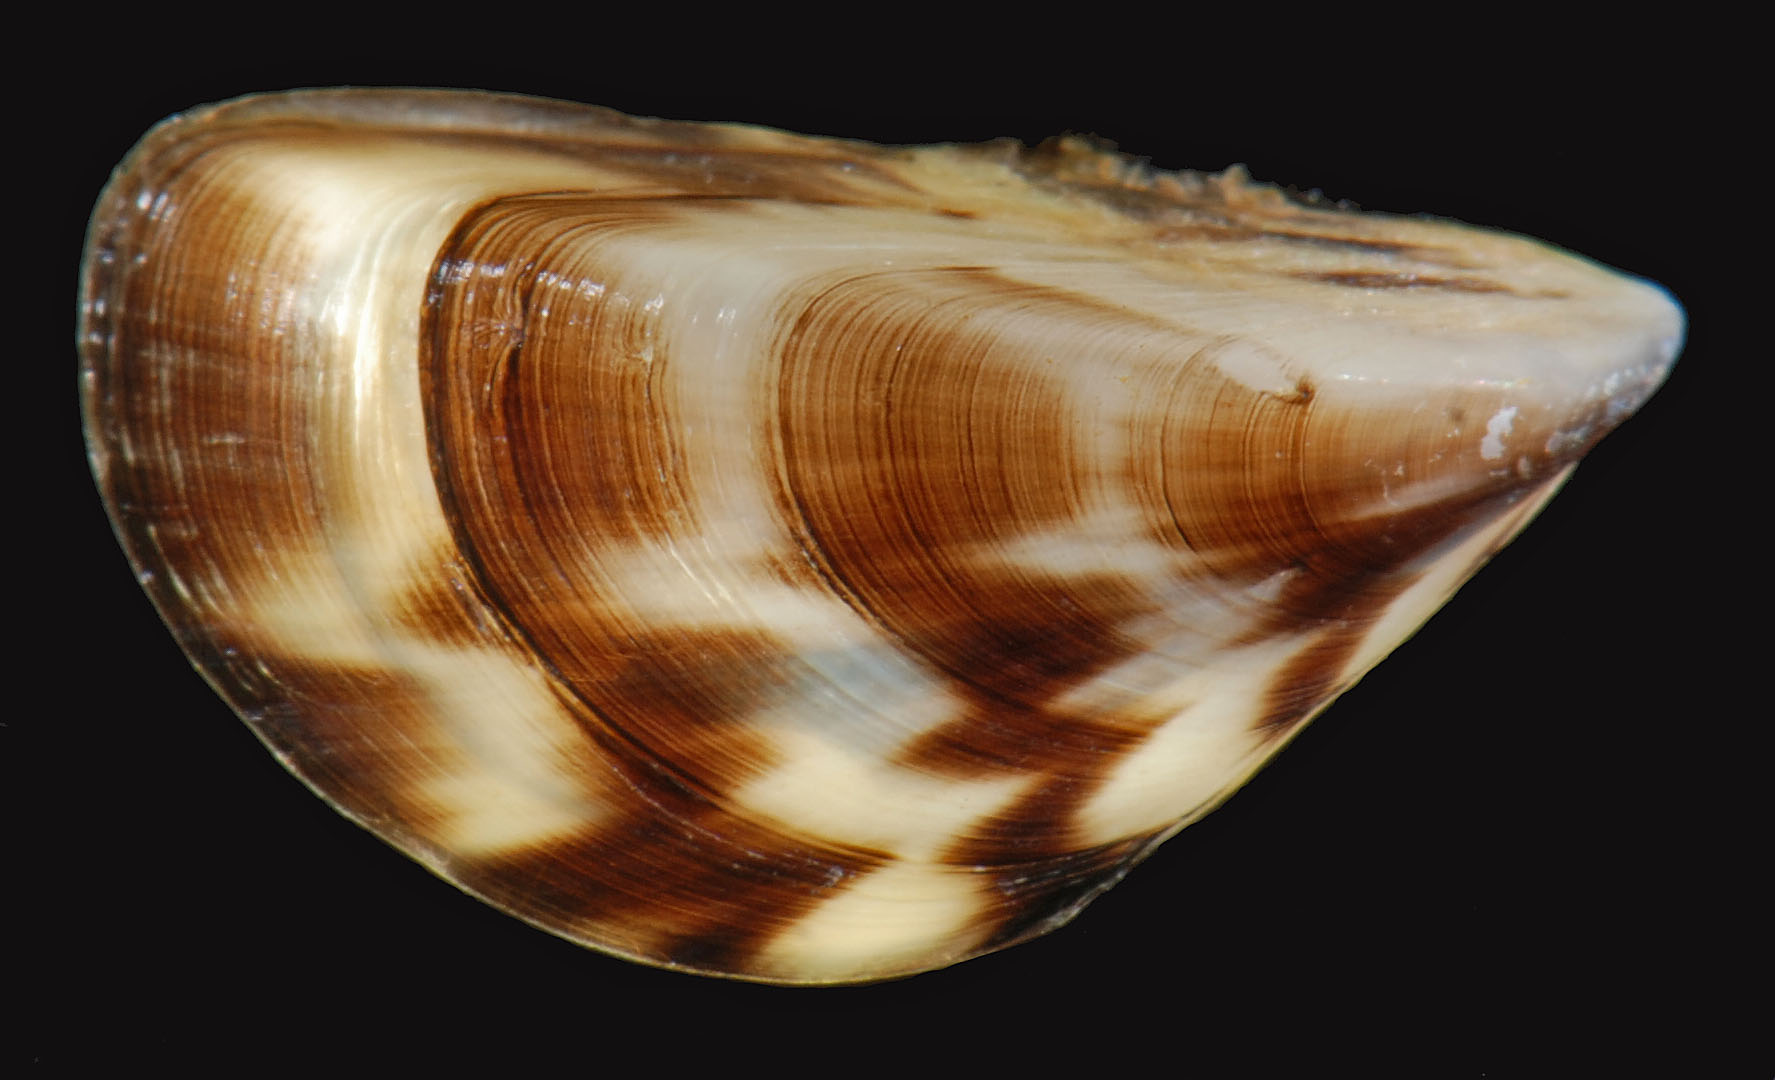
\includegraphics[width=0.28\textwidth]{../data/taxa_images/Dreissena_image.jpg}
    \caption{Dreissena}
    \label{fig:dreissena}
\end{wrapfigure}
\noindent\textbf{Dreissena} (F = 86.56***) exhibited the most significant difference among clusters, with extremely high abundance in Cluster 0 (3.982) but nearly absent in Clusters 1 (0.114) and 2 (0.495). Zebra and quagga mussels strongly characterize hard substrate environments with good water circulation. These invasive bivalves are filter feeders that can significantly alter local nutrient dynamics and water clarity. Their presence typically indicates stable, hard substrates such as rocks, cobbles, or artificial structures. \lipsum[1][1-4]

\begin{wrapfigure}{l}{0.3\textwidth}
    \centering
    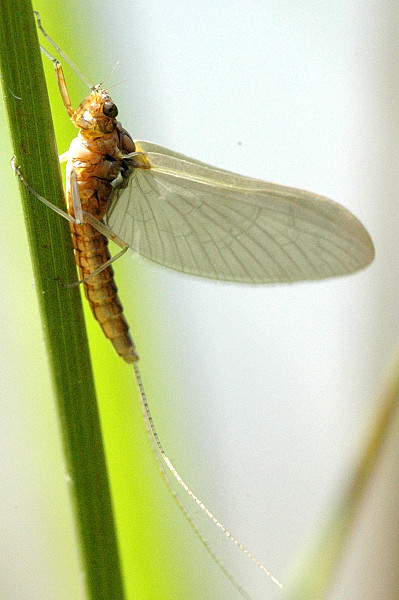
\includegraphics[width=0.28\textwidth]{../data/taxa_images/Caenis_image.jpg}
    \caption{Caenis}
    \label{fig:caenis}
\end{wrapfigure}
\noindent\textbf{Caenis} (F = 57.94***) was predominantly found in Cluster 2 (2.892) with minimal presence in Clusters 0 (0.134) and 1 (0.088). These small mayflies are characteristic of erosional, shallow-water environments with moderate current. They are collector-gatherers that feed on fine particulate organic matter and are moderately tolerant to pollution, making them useful indicators of intermediate water quality conditions in lotic systems. \lipsum[2][1-4]

\lipsum[2]

\begin{wrapfigure}{r}{0.3\textwidth}
    \centering
    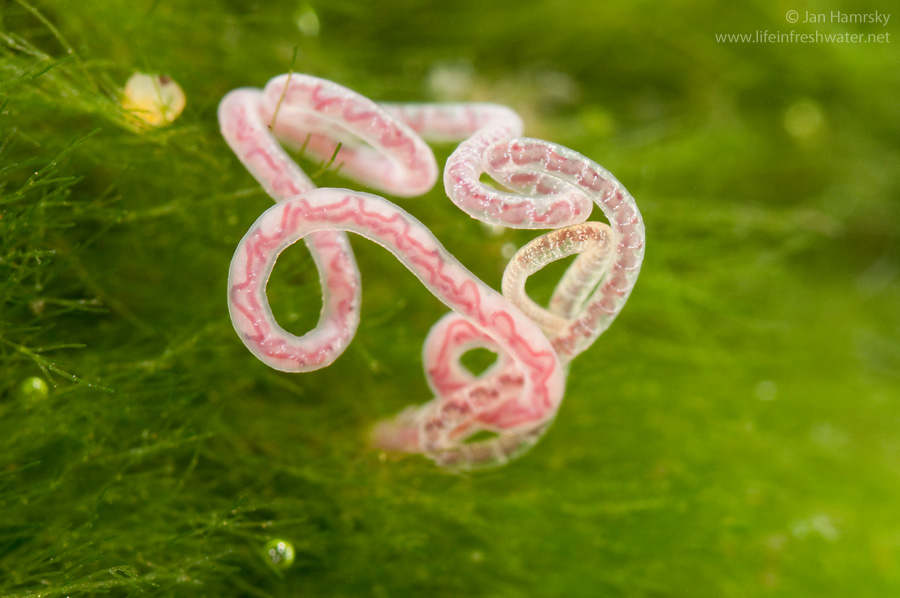
\includegraphics[width=0.28\textwidth]{../data/taxa_images/Oligochaeta_image.jpg}
    \caption{Oligochaeta}
    \label{fig:oligochaeta}
\end{wrapfigure}
noindent\textbf{Oligochaeta} (F = 17.52***) showed the highest abundance in Cluster 1 (5.614) compared to Cluster 0 (3.964) and Cluster 2 (4.337). These segmented worms are important indicators of organic enrichment in fine-grained sediments. They play a crucial role in sediment bioturbation and nutrient cycling, and their high abundance often indicates depositional environments with accumulated organic matter. \lipsum[3][1-4]


\begin{wrapfigure}{l}{0.3\textwidth}
    \centering
    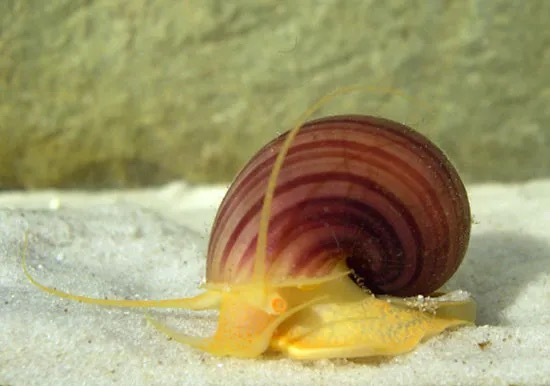
\includegraphics[width=0.28\textwidth]{../data/taxa_images/Gastropoda_image_converted.jpg}
    \caption{Gastropoda}
    \label{fig:gastropoda}
\end{wrapfigure}
\noindent\textbf{Gastropoda} (F = 16.36***) showed highest abundance in Cluster 2 (2.957), moderate in Cluster 0 (0.940), and lowest in Cluster 1 (0.373). Freshwater snails prefer hard substrates and well-oxygenated shallow waters where they graze on periphyton and detritus. Their distribution patterns often reflect substrate type, food availability, and calcium concentrations in the benthic environment. \lipsum[4][1-4]

\begin{wrapfigure}{r}{0.3\textwidth}
    \centering
    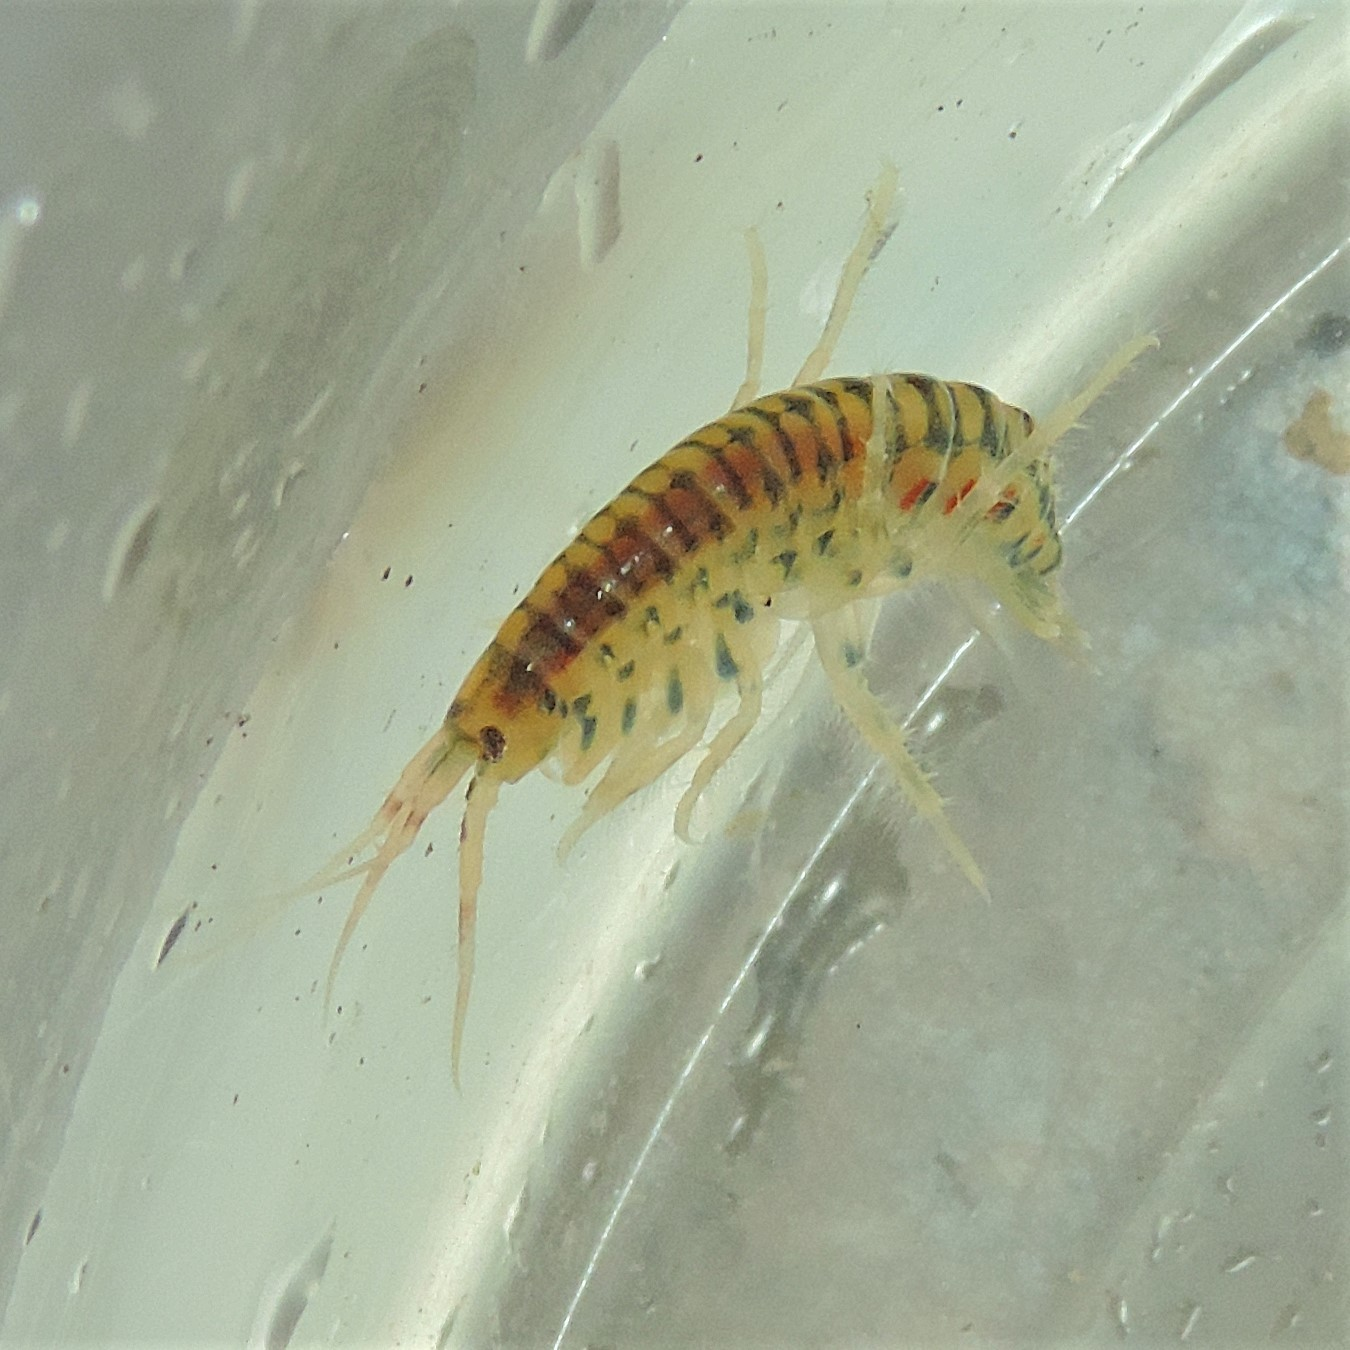
\includegraphics[width=0.28\textwidth]{../data/taxa_images/Amphipoda_image.jpg}
    \caption{Amphipoda}
    \label{fig:amphipoda}
\end{wrapfigure}
\noindent\textbf{Amphipoda} (F = 10.27***) was most abundant in Cluster 0 (1.728), moderate in Cluster 2 (1.227), and nearly absent in Cluster 1 (0.150). Scuds are sensitive indicators preferring clean, well-oxygenated habitats with structured substrates. They are important prey items for fish and serve as shredders and detritivores in the benthic food web, processing coarse particulate organic matter. \lipsum[5][1-4]

\begin{wrapfigure}{l}{0.3\textwidth}
    \centering
    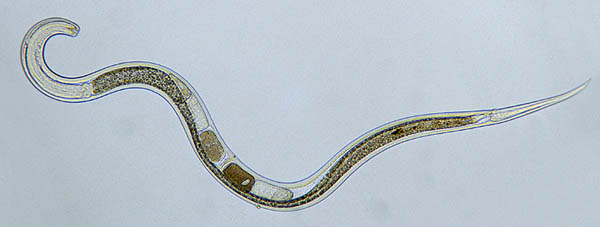
\includegraphics[width=0.28\textwidth]{../data/taxa_images/Nematoda_image.jpg}
    \caption{Nematoda}
    \label{fig:nematoda}
\end{wrapfigure}
\noindent\textbf{Nematoda} (F = 5.71**) decreased progressively from Cluster 0 (3.478) to Cluster 1 (2.468) to Cluster 2 (1.283). Roundworms show distinct habitat preferences based on sediment characteristics and organic matter content. They occupy multiple trophic levels as bacterivores, fungivores, and predators, making them important components of the meiofaunal community in aquatic sediments. \lipsum[6][1-4]

\begin{wrapfigure}{r}{0.3\textwidth}
    \centering
    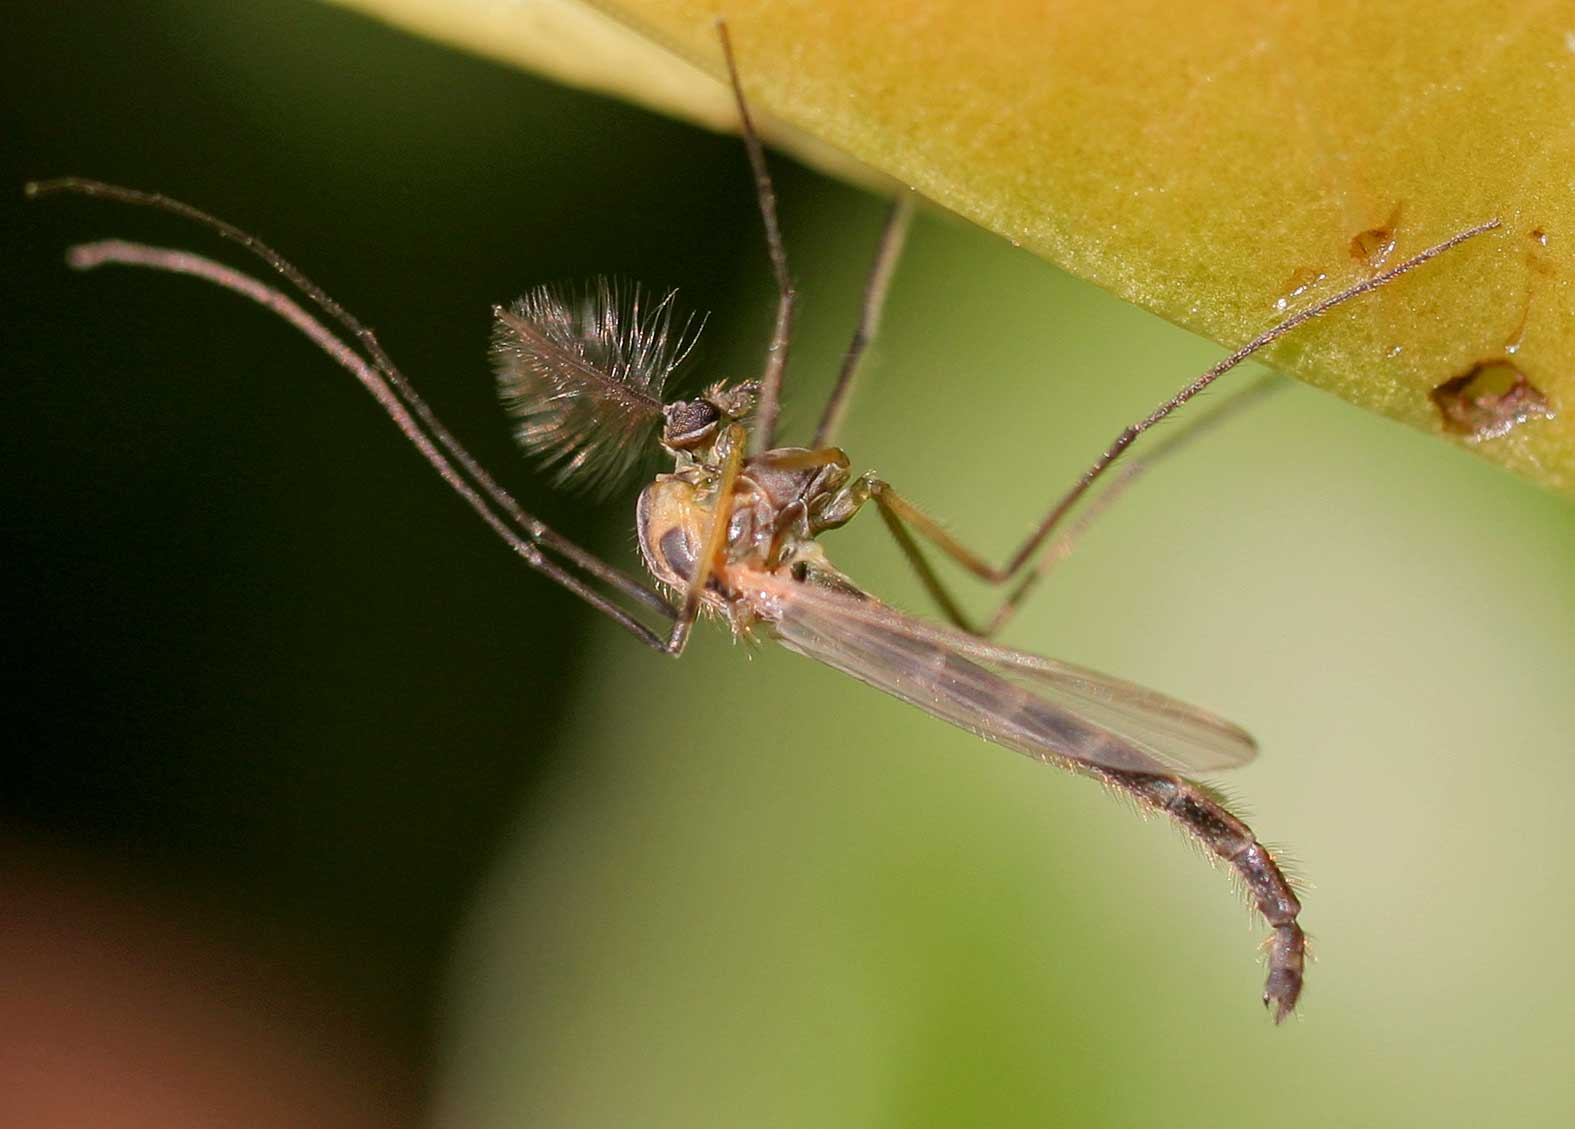
\includegraphics[width=0.28\textwidth]{../data/taxa_images/Chironomidae_image.jpg}
    \caption{Chironomidae}
    \label{fig:chironomidae}
\end{wrapfigure}
\noindent\textbf{Chironomidae} (F = 4.90*) showed lowest abundance in Cluster 0 (3.365) compared to Clusters 1 (4.689) and 2 (4.471). Non-biting midge larvae occupy a wide range of habitats with varying pollution tolerances. Different chironomid subfamilies and genera show distinct environmental preferences, making them valuable bioindicators when identified to lower taxonomic levels. \lipsum[7][1-4]




\chapter{Environment Driven Taxa Clusters}

%% ============================================
%% RDA Analysis Tables
%% ============================================

\begin{table}[htbp]
    \centering
    \caption{RDA Axes Summary}
    \label{tab:03_rda_axes}
    \small
    \begin{tabular}{lccccc}
        \toprule
        \textbf{Axis} & \textbf{Eigenvalue} & \textbf{Expl. (\%)} & \textbf{Cumul. (\%)} & \textbf{F-stat} & \textbf{p-value} \\
        \midrule
        RDA1 & 0.0295 & 44.53 & 44.53 & 5.789 & 0.001$^{**}$ \\
        RDA2 & 0.0155 & 23.42 & 67.95 & 3.044 & 0.151 \\
        RDA3 & 0.0119 & 17.98 & 85.93 & 2.338 & 0.483 \\
        RDA4 & 0.0047 & 7.15 & 93.08 & 0.929 & 1.000 \\
        RDA5 & 0.0026 & 3.98 & 97.06 & 0.517 & 1.000 \\
        RDA6 & 0.0020 & 2.94 & 100.00 & 0.383 & 1.000 \\
        \bottomrule
    \end{tabular}
    
    \vspace{0.5em}
    \footnotesize
    \textit{Note:} Permutations = 999; $R^2$ = 0.2167; Adjusted $R^2$ = 0.1167; Global test p-value = 0.0010$^{**}$
\end{table}

\begin{table}[htbp]
    \centering
    \caption{RDA Environmental Terms}
    \label{tab:03_rda_env_terms}
    \small
    \begin{tabular}{l@{\hspace{8pt}}c@{\hspace{8pt}}c@{\hspace{8pt}}c@{\hspace{8pt}}r@{\hspace{8pt}}r}
        \toprule
        \textbf{Variable} & \textbf{$\Delta$ Inertia} & \textbf{F-stat} & \textbf{p-value} & \textbf{RDA1} & \textbf{RDA2} \\
        \midrule
        MPS (Phi) & 1.204 & 4.459 & 0.001$^{**}$ & $-0.900$ & 0.088 \\
        Velocity (m/sec) & 0.624 & 2.310 & 0.016$^{*}$ & 0.361 & 0.165 \\
        Depth (m) & 0.478 & 1.769 & 0.065 & 0.456 & $-0.442$ \\
        Temperature (\textdegree C) & 0.424 & 1.572 & 0.112 & $-0.046$ & 0.699 \\
        DO Bottom (mg/L) & 0.340 & 1.258 & 0.235 & $-0.108$ & $-0.628$ \\
        LOI (\%) & 0.185 & 0.684 & 0.747 & 0.136 & 0.228 \\
        \bottomrule
    \end{tabular}
\end{table}

\begin{figure}[htbp]
    \centering
    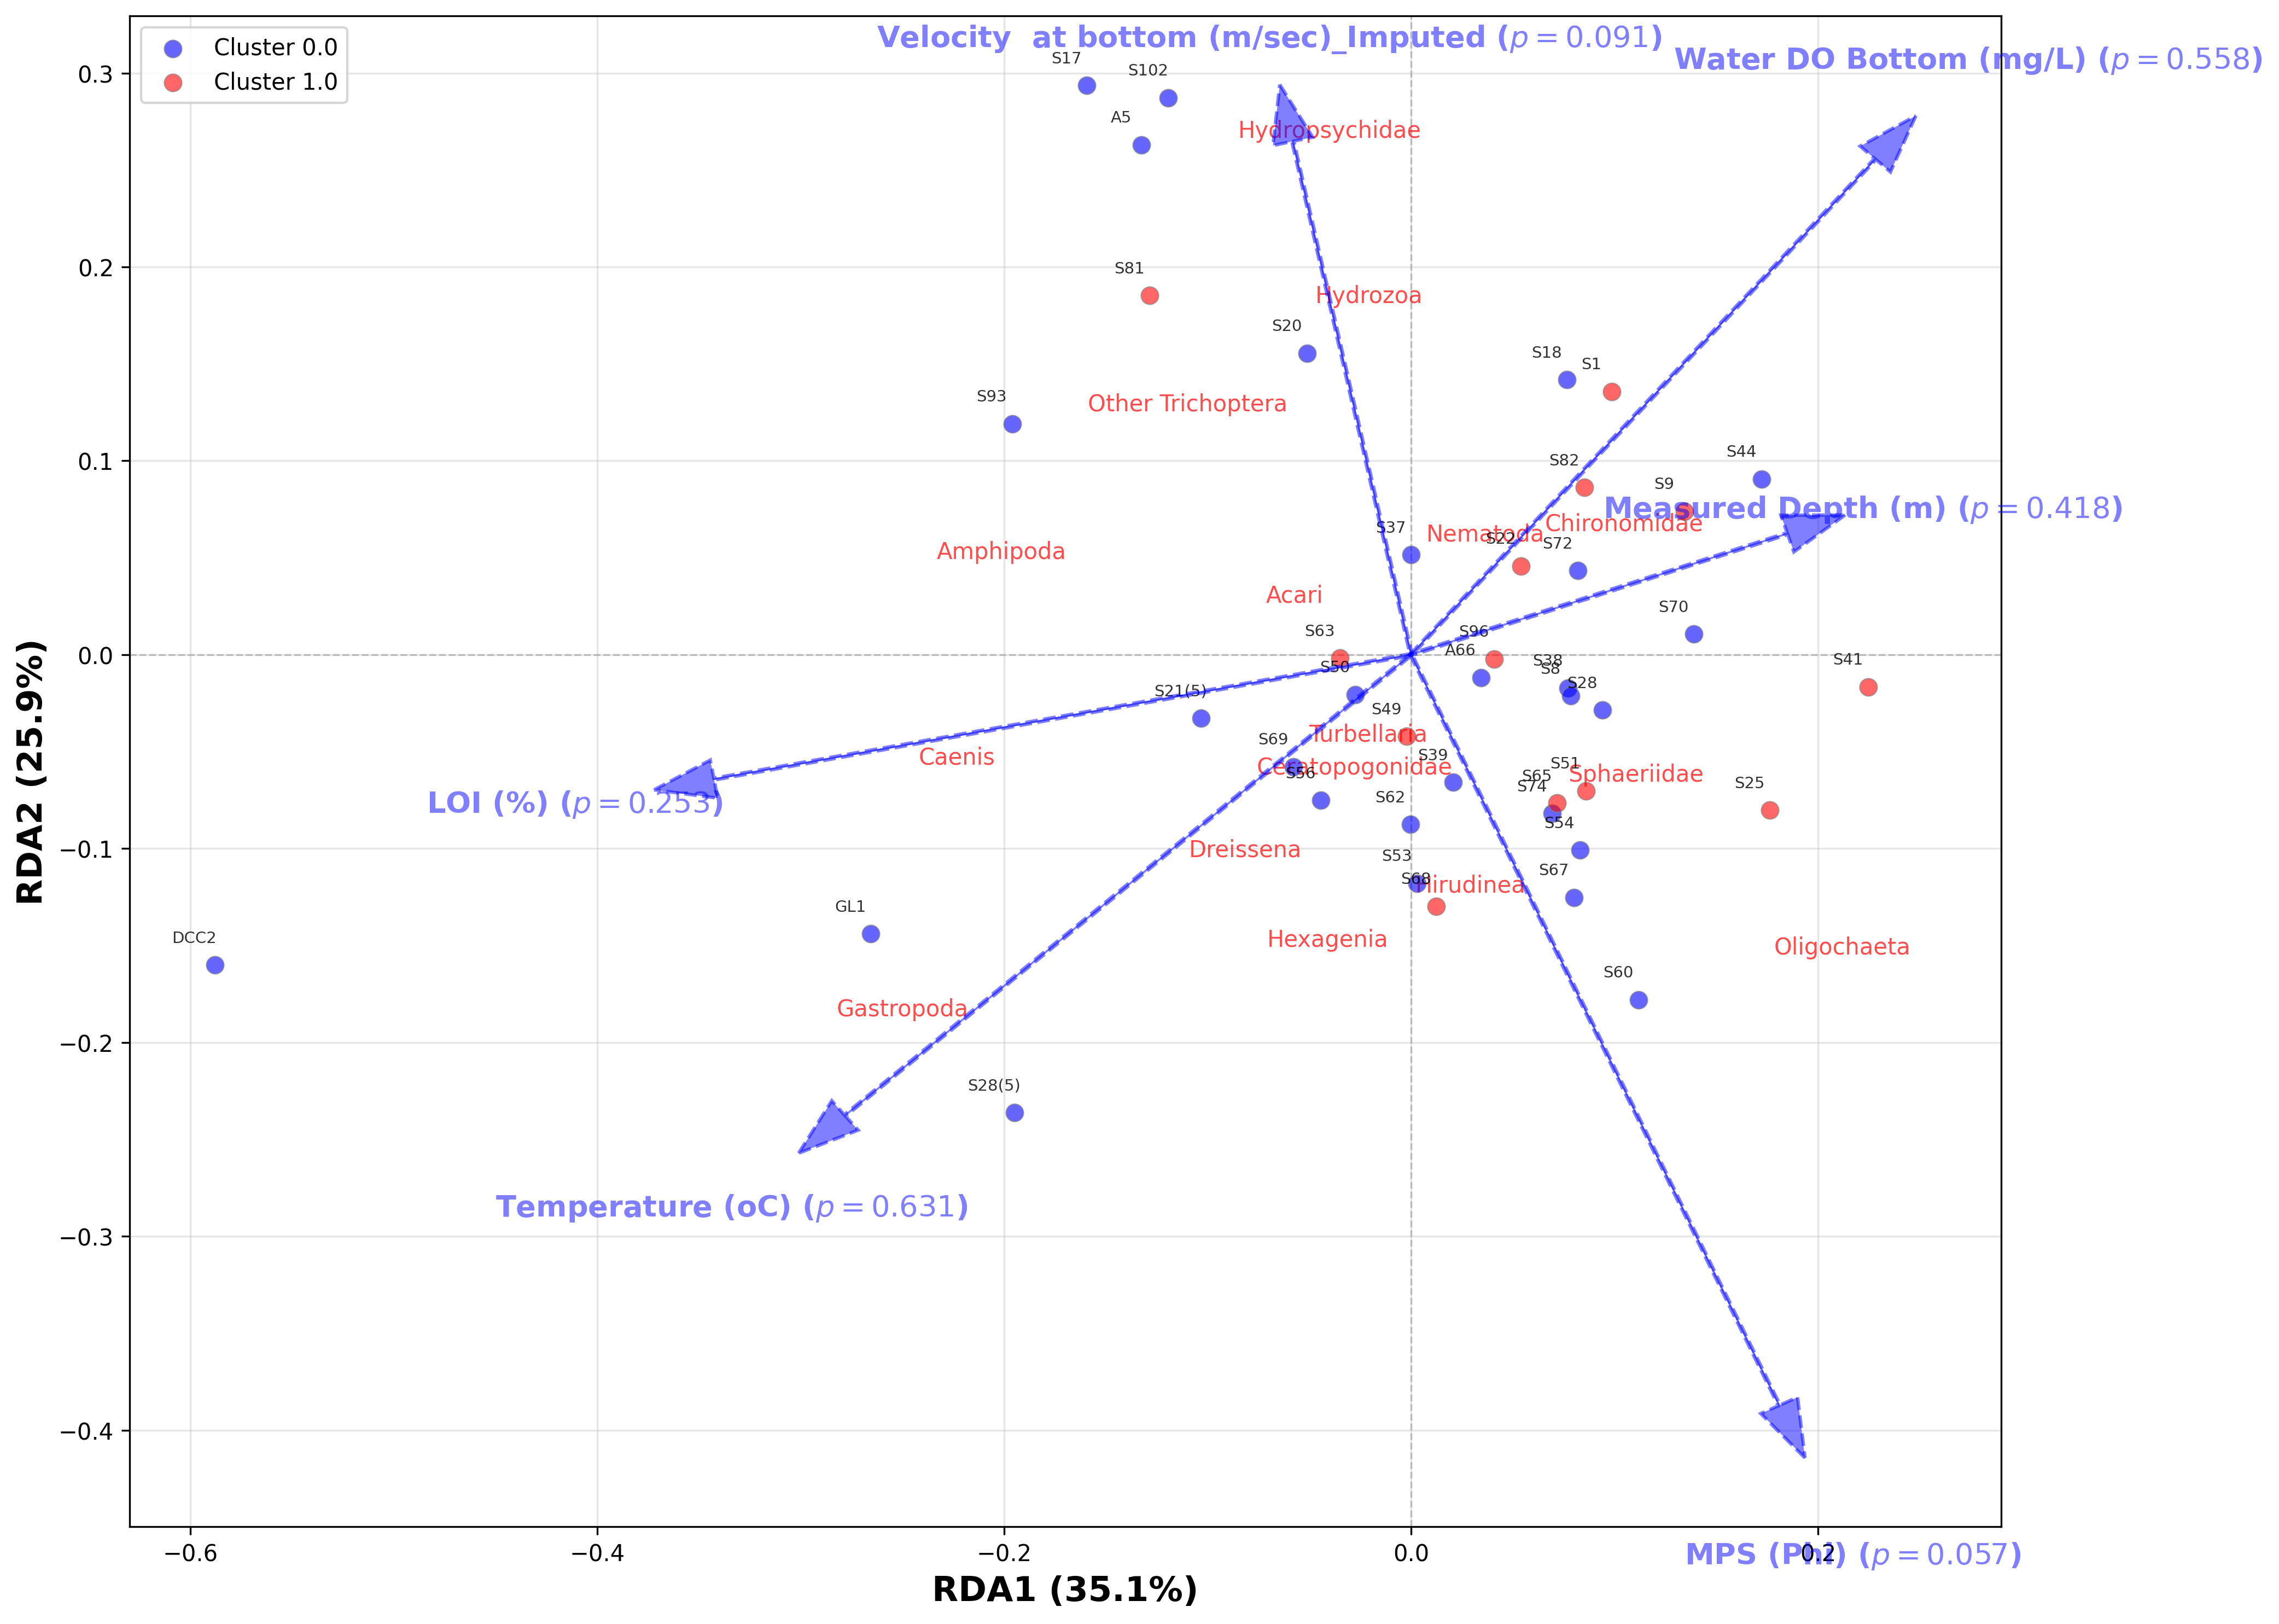
\includegraphics[width=0.9\textwidth]{../results/figures/03_env_driven_taxa_clusters/figure1_rda_triplot.png}
    \caption{RDA Triplot}
    \label{fig:03_rda_triplot}
\end{figure}

% \begin{figure}[htbp]
%     \centering
%     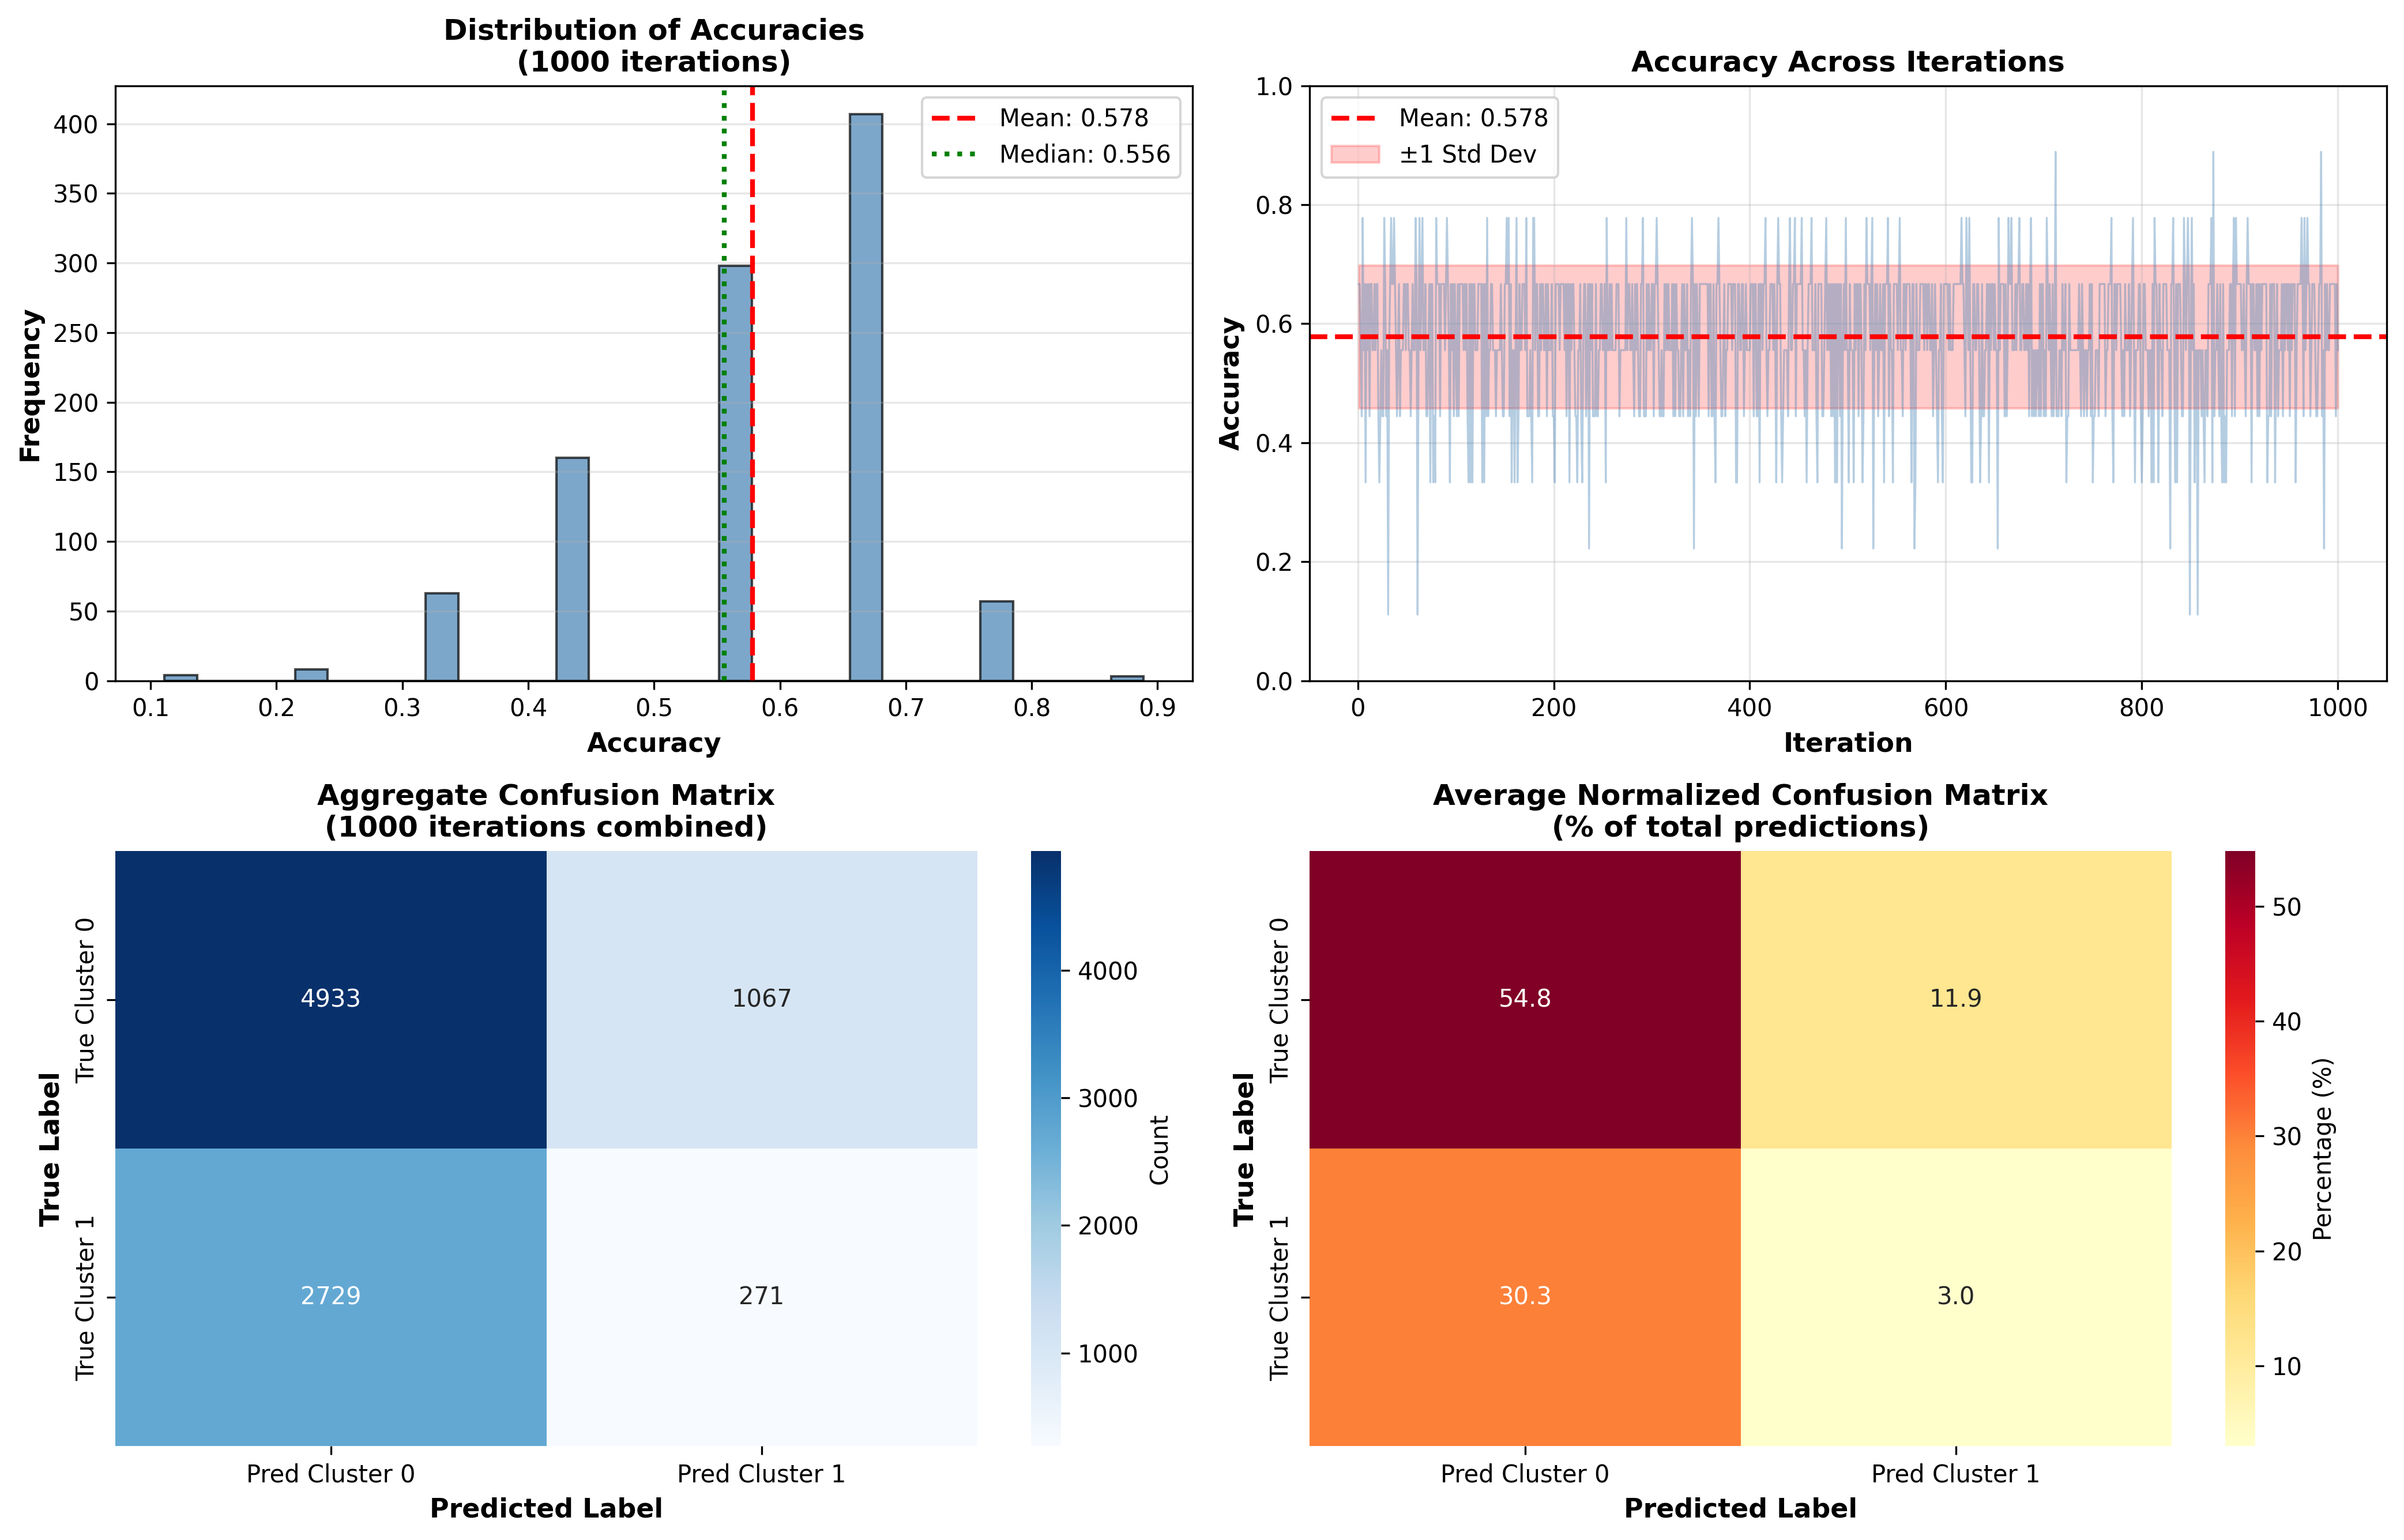
\includegraphics[width=0.9\textwidth]{../results/figures/03_env_driven_taxa_clusters/figure2_lda_cv.png}
%     \caption{LDA Cross-Validation}
%     \label{fig:03_lda_cv}
% \end{figure}

%% ============================================
%% LDA Analysis Tables
%% ============================================

\begin{table}[htbp]
    \centering
    \caption{LDA Variable Importance (Wilks' Lambda) and Discriminant Axes Summary}
    \label{tab:03_lda_analysis}
    \small
    \begin{tabular}{l@{\hspace{8pt}}c@{\hspace{8pt}}c@{\hspace{8pt}}c@{\hspace{8pt}}r@{\hspace{8pt}}r}
        \toprule
        \textbf{Variable} & \textbf{$\Delta\Lambda$} & \textbf{F-stat} & \textbf{p-value} & \textbf{LD1} & \textbf{LD2} \\
        \midrule
        MPS (Phi) & 0.130 & 6.926 & 0.002$^{**}$ & $-0.924$ & 0.666 \\
        Temperature (\textdegree C) & 0.119 & 6.336 & 0.004$^{**}$ & 0.388 & $-0.667$ \\
        Velocity (m/sec) & 0.104 & 5.534 & 0.007$^{**}$ & $-0.781$ & 0.185 \\
        Depth (m) & 0.087 & 4.617 & 0.015$^{*}$ & 0.552 & $-0.010$ \\
        DO Bottom (mg/L) & 0.022 & 1.186 & 0.315 & 0.088 & 0.156 \\
        LOI (\%) & 0.000 & 0.024 & 0.976 & $-0.021$ & $-0.013$ \\
        \midrule
        \textbf{Explained (\%)} & -- & -- & -- & 59.44 & 40.56 \\
        \textbf{Cumulative (\%)} & -- & -- & -- & 59.44 & 100.00 \\
        \bottomrule
    \end{tabular}
\end{table}

%% ============================================
%% LDA Classification Results
%% ============================================

\begin{table}[htbp]
    \centering
    \caption{LDA Classification Confusion Matrix (Training Data)}
    \label{tab:03_lda_confusion}
    \small
    \begin{tabular}{lccc}
        \toprule
        & \textbf{Pred. Cluster 0} & \textbf{Pred. Cluster 1} & \textbf{Pred. Cluster 2} \\
        \midrule
        True Cluster 0 & 12 & 5 & 1 \\
        True Cluster 1 & 3 & 25 & 0 \\
        True Cluster 2 & 1 & 3 & 4 \\
        \bottomrule
    \end{tabular}
\end{table}

\begin{table}[htbp]
    \centering
    \caption{LDA Classification Report (Training Data)}
    \label{tab:03_lda_classification}
    \small
    \begin{tabular}{lcccc}
        \toprule
        & \textbf{Precision} & \textbf{Recall} & \textbf{F1-Score} & \textbf{Support} \\
        \midrule
        Cluster 0 & 0.75 & 0.67 & 0.71 & 18 \\
        Cluster 1 & 0.76 & 0.89 & 0.82 & 28 \\
        Cluster 2 & 0.80 & 0.50 & 0.62 & 8 \\
        \midrule
        Accuracy & -- & -- & 0.76 & 54 \\
        Macro avg & 0.77 & 0.69 & 0.71 & 54 \\
        Weighted avg & 0.76 & 0.76 & 0.75 & 54 \\
        \bottomrule
    \end{tabular}
    
    \vspace{0.5em}
    \footnotesize
    \textit{Note:} Overall Accuracy = 0.7593; Number of sites = 54
\end{table}

%% ============================================
%% LDA Monte Carlo Cross-Validation Results
%% ============================================
\begin{table}[htbp]
    \centering
    \caption{LDA Monte Carlo Cross-Validation Aggregate Confusion Matrix (Test Size: 20.0\% per 1000 iteration)}
    \label{tab:03_lda_cv_confusion_aggregate}
    \small
    \begin{tabular}{lccc}
        \toprule
        & \textbf{Pred. Cluster 0} & \textbf{Pred. Cluster 1} & \textbf{Pred. Cluster 2} \\
        \midrule
        True Cluster 0 & 2178 & 1486 & 336 \\
        True Cluster 1 & 944 & 4901 & 155 \\
        True Cluster 2 & 237 & 389 & 374 \\
        \bottomrule
    \end{tabular}
    
    \vspace{0.5em}
    \footnotesize
    \textit{Note:} Combined results from 1,000 cross-validation iterations
\end{table}

\begin{table}[htbp]
    \centering
    \caption{LDA Monte Carlo Cross-Validation Results Summary (Test Size: 20.0\% per 1000 iteration)}
    \label{tab:03_lda_cv_results}
    \small
    \begin{tabular}{l@{\hspace{12pt}}c@{\hspace{8pt}}c@{\hspace{8pt}}c@{\hspace{8pt}}c}
        \toprule
        \multicolumn{5}{c}{\textbf{Average Classification Performance}} \\
        \midrule
        \textbf{Class} & \textbf{Precision} & \textbf{Recall} & \textbf{F1-Score} & \textbf{Support} \\
        \midrule
        Cluster 0 & 0.645 $\pm$ 0.275 & 0.544 $\pm$ 0.278 & 0.560 $\pm$ 0.236 & 18 \\
        Cluster 1 & 0.743 $\pm$ 0.134 & 0.817 $\pm$ 0.155 & 0.766 $\pm$ 0.108 & 28 \\
        Cluster 2 & 0.267 $\pm$ 0.384 & 0.374 $\pm$ 0.484 & 0.300 $\pm$ 0.406 & 8 \\
        \midrule
        Weighted Avg & 0.664 $\pm$ 0.157 & 0.678 $\pm$ 0.123 & 0.649 $\pm$ 0.136 & 54 \\
        \midrule
        \midrule
        \multicolumn{2}{l}{Mean accuracy} & \multicolumn{3}{c}{0.6775 $\pm$ 0.1228} \\
        \multicolumn{2}{l}{Median accuracy} & \multicolumn{3}{c}{0.7273} \\
        \bottomrule
    \end{tabular}
    
    \vspace{0.5em}
    \footnotesize
    \textit{Note:} Classification metrics shown as mean $\pm$ standard deviation across 1,000 CV iterations
\end{table}

% \begin{figure}[htbp]
%     \centering
%     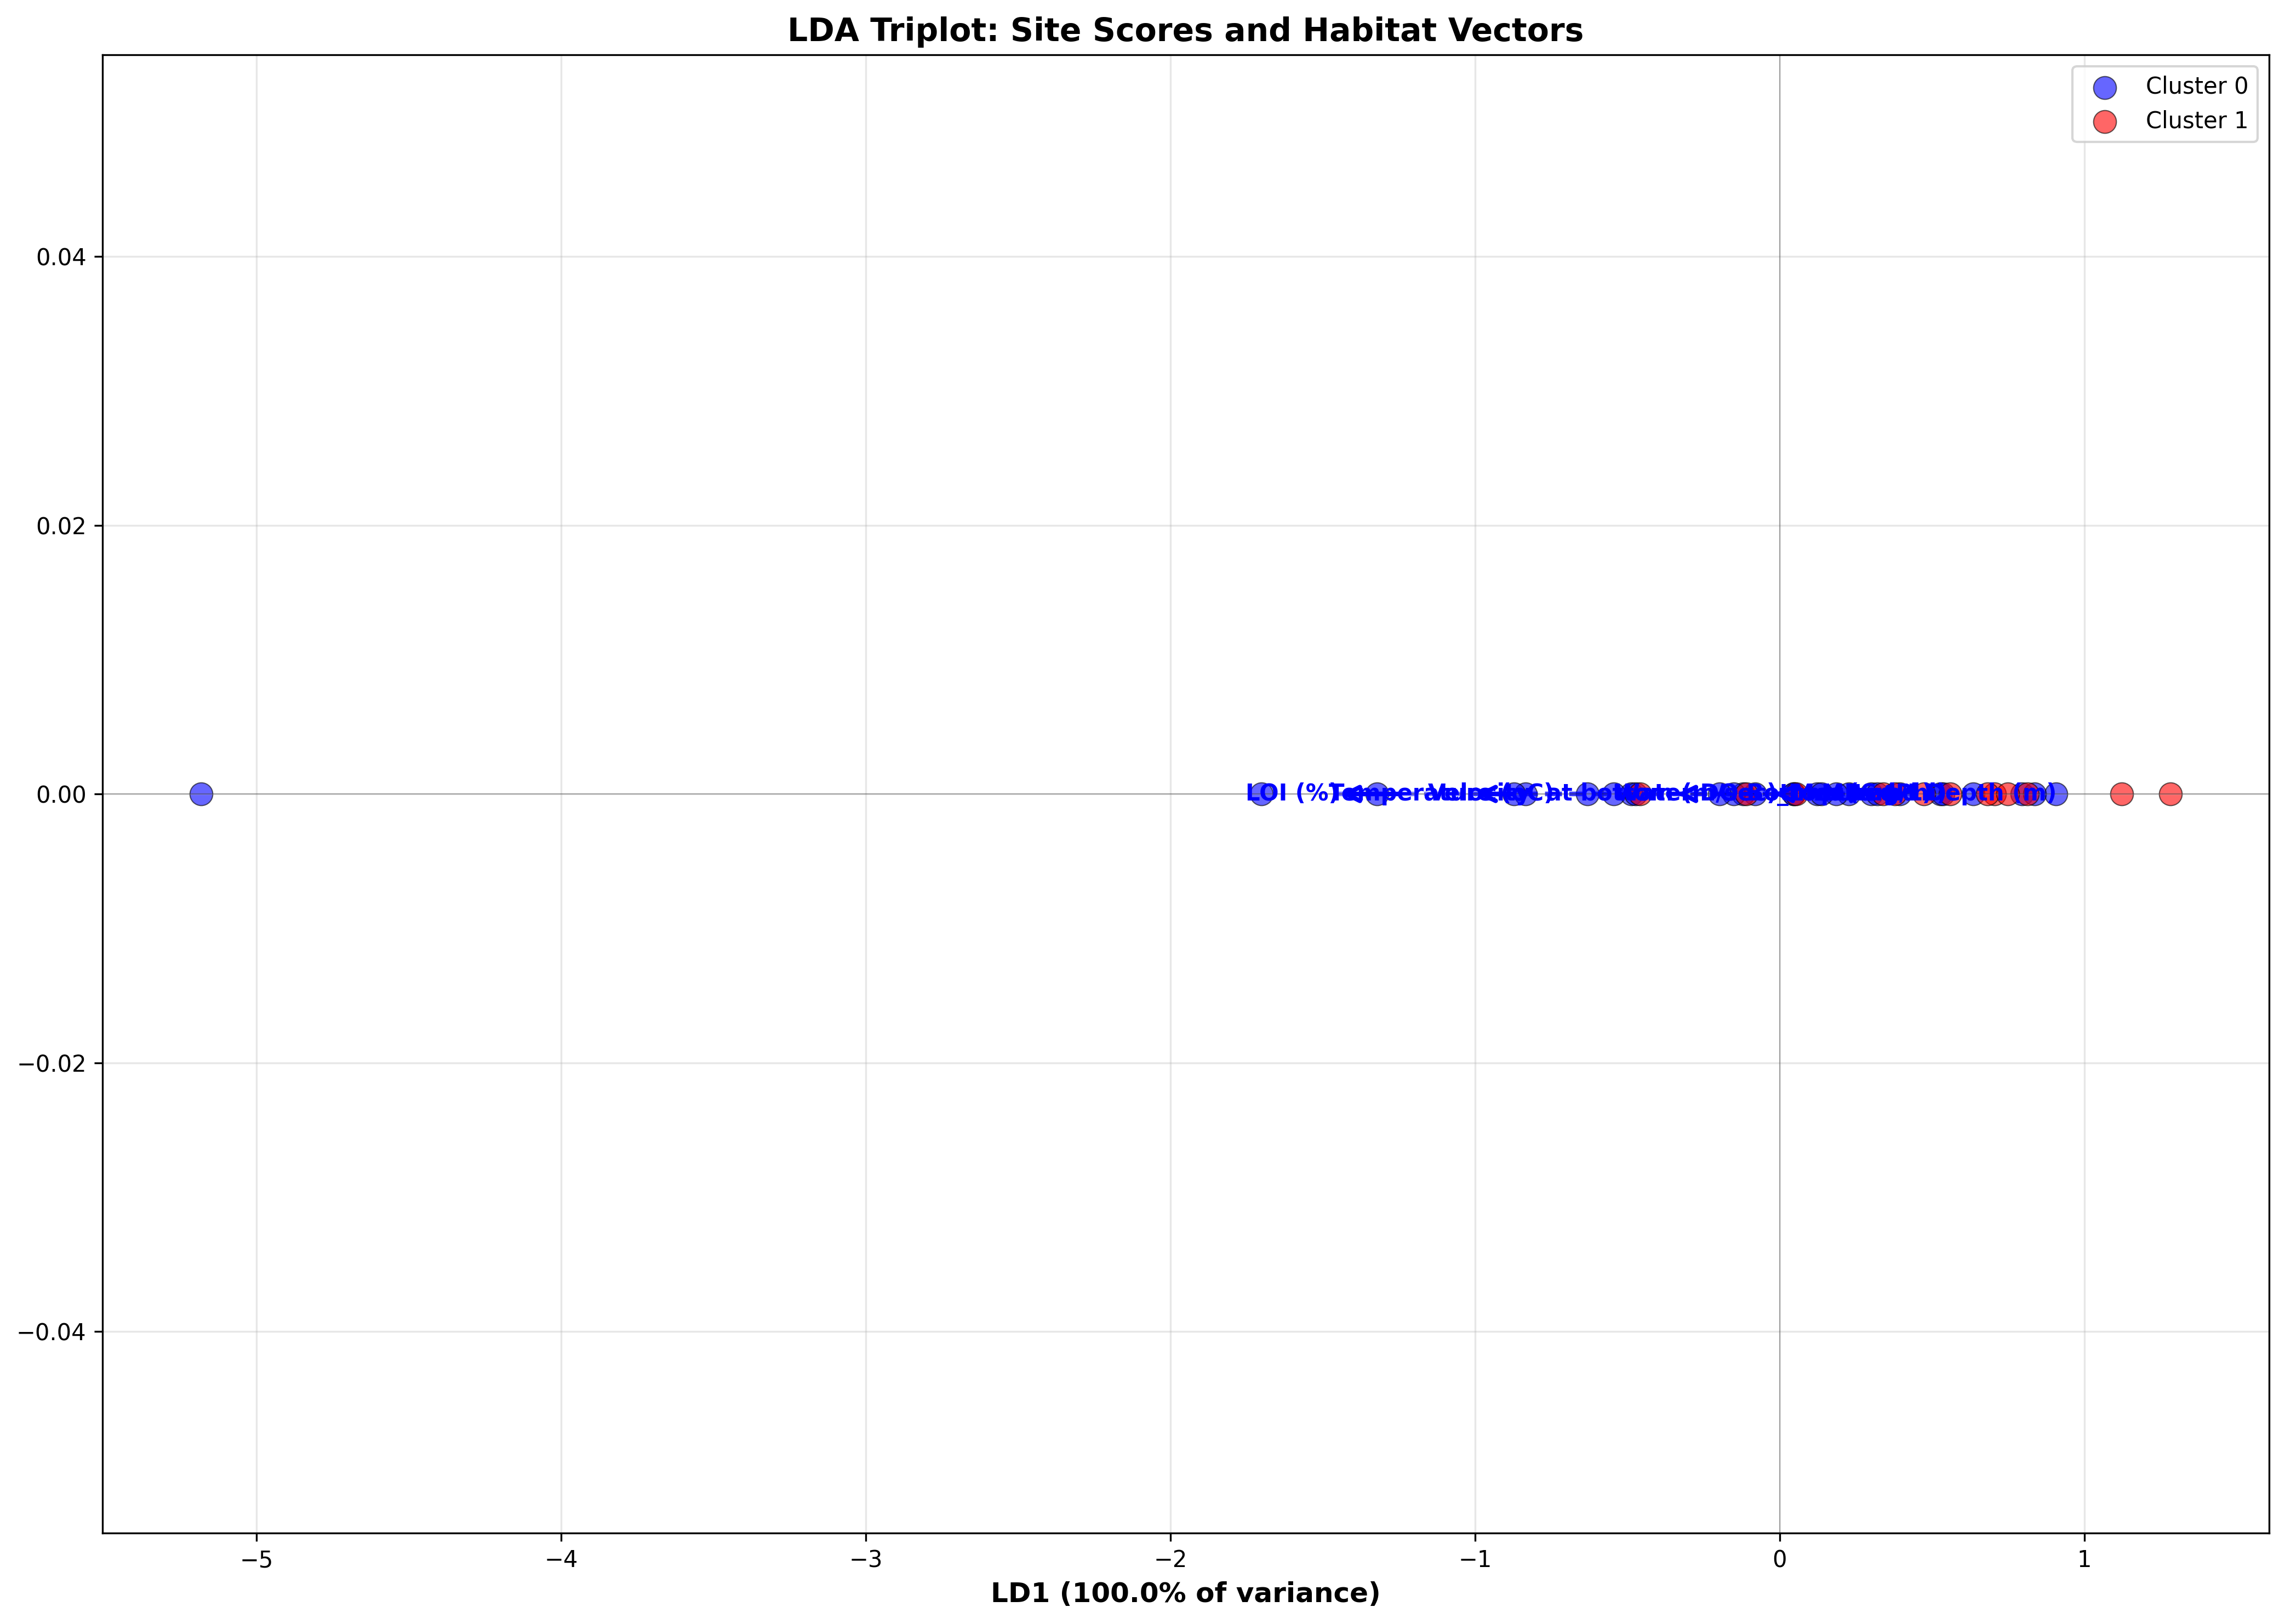
\includegraphics[width=0.9\textwidth]{../results/figures/03_env_driven_taxa_clusters/figure3_lda_triplot.png}
%     \caption{LDA Triplot}
%     \label{fig:03_lda_triplot}
% \end{figure}

\begin{figure}[htbp]
    \centering
    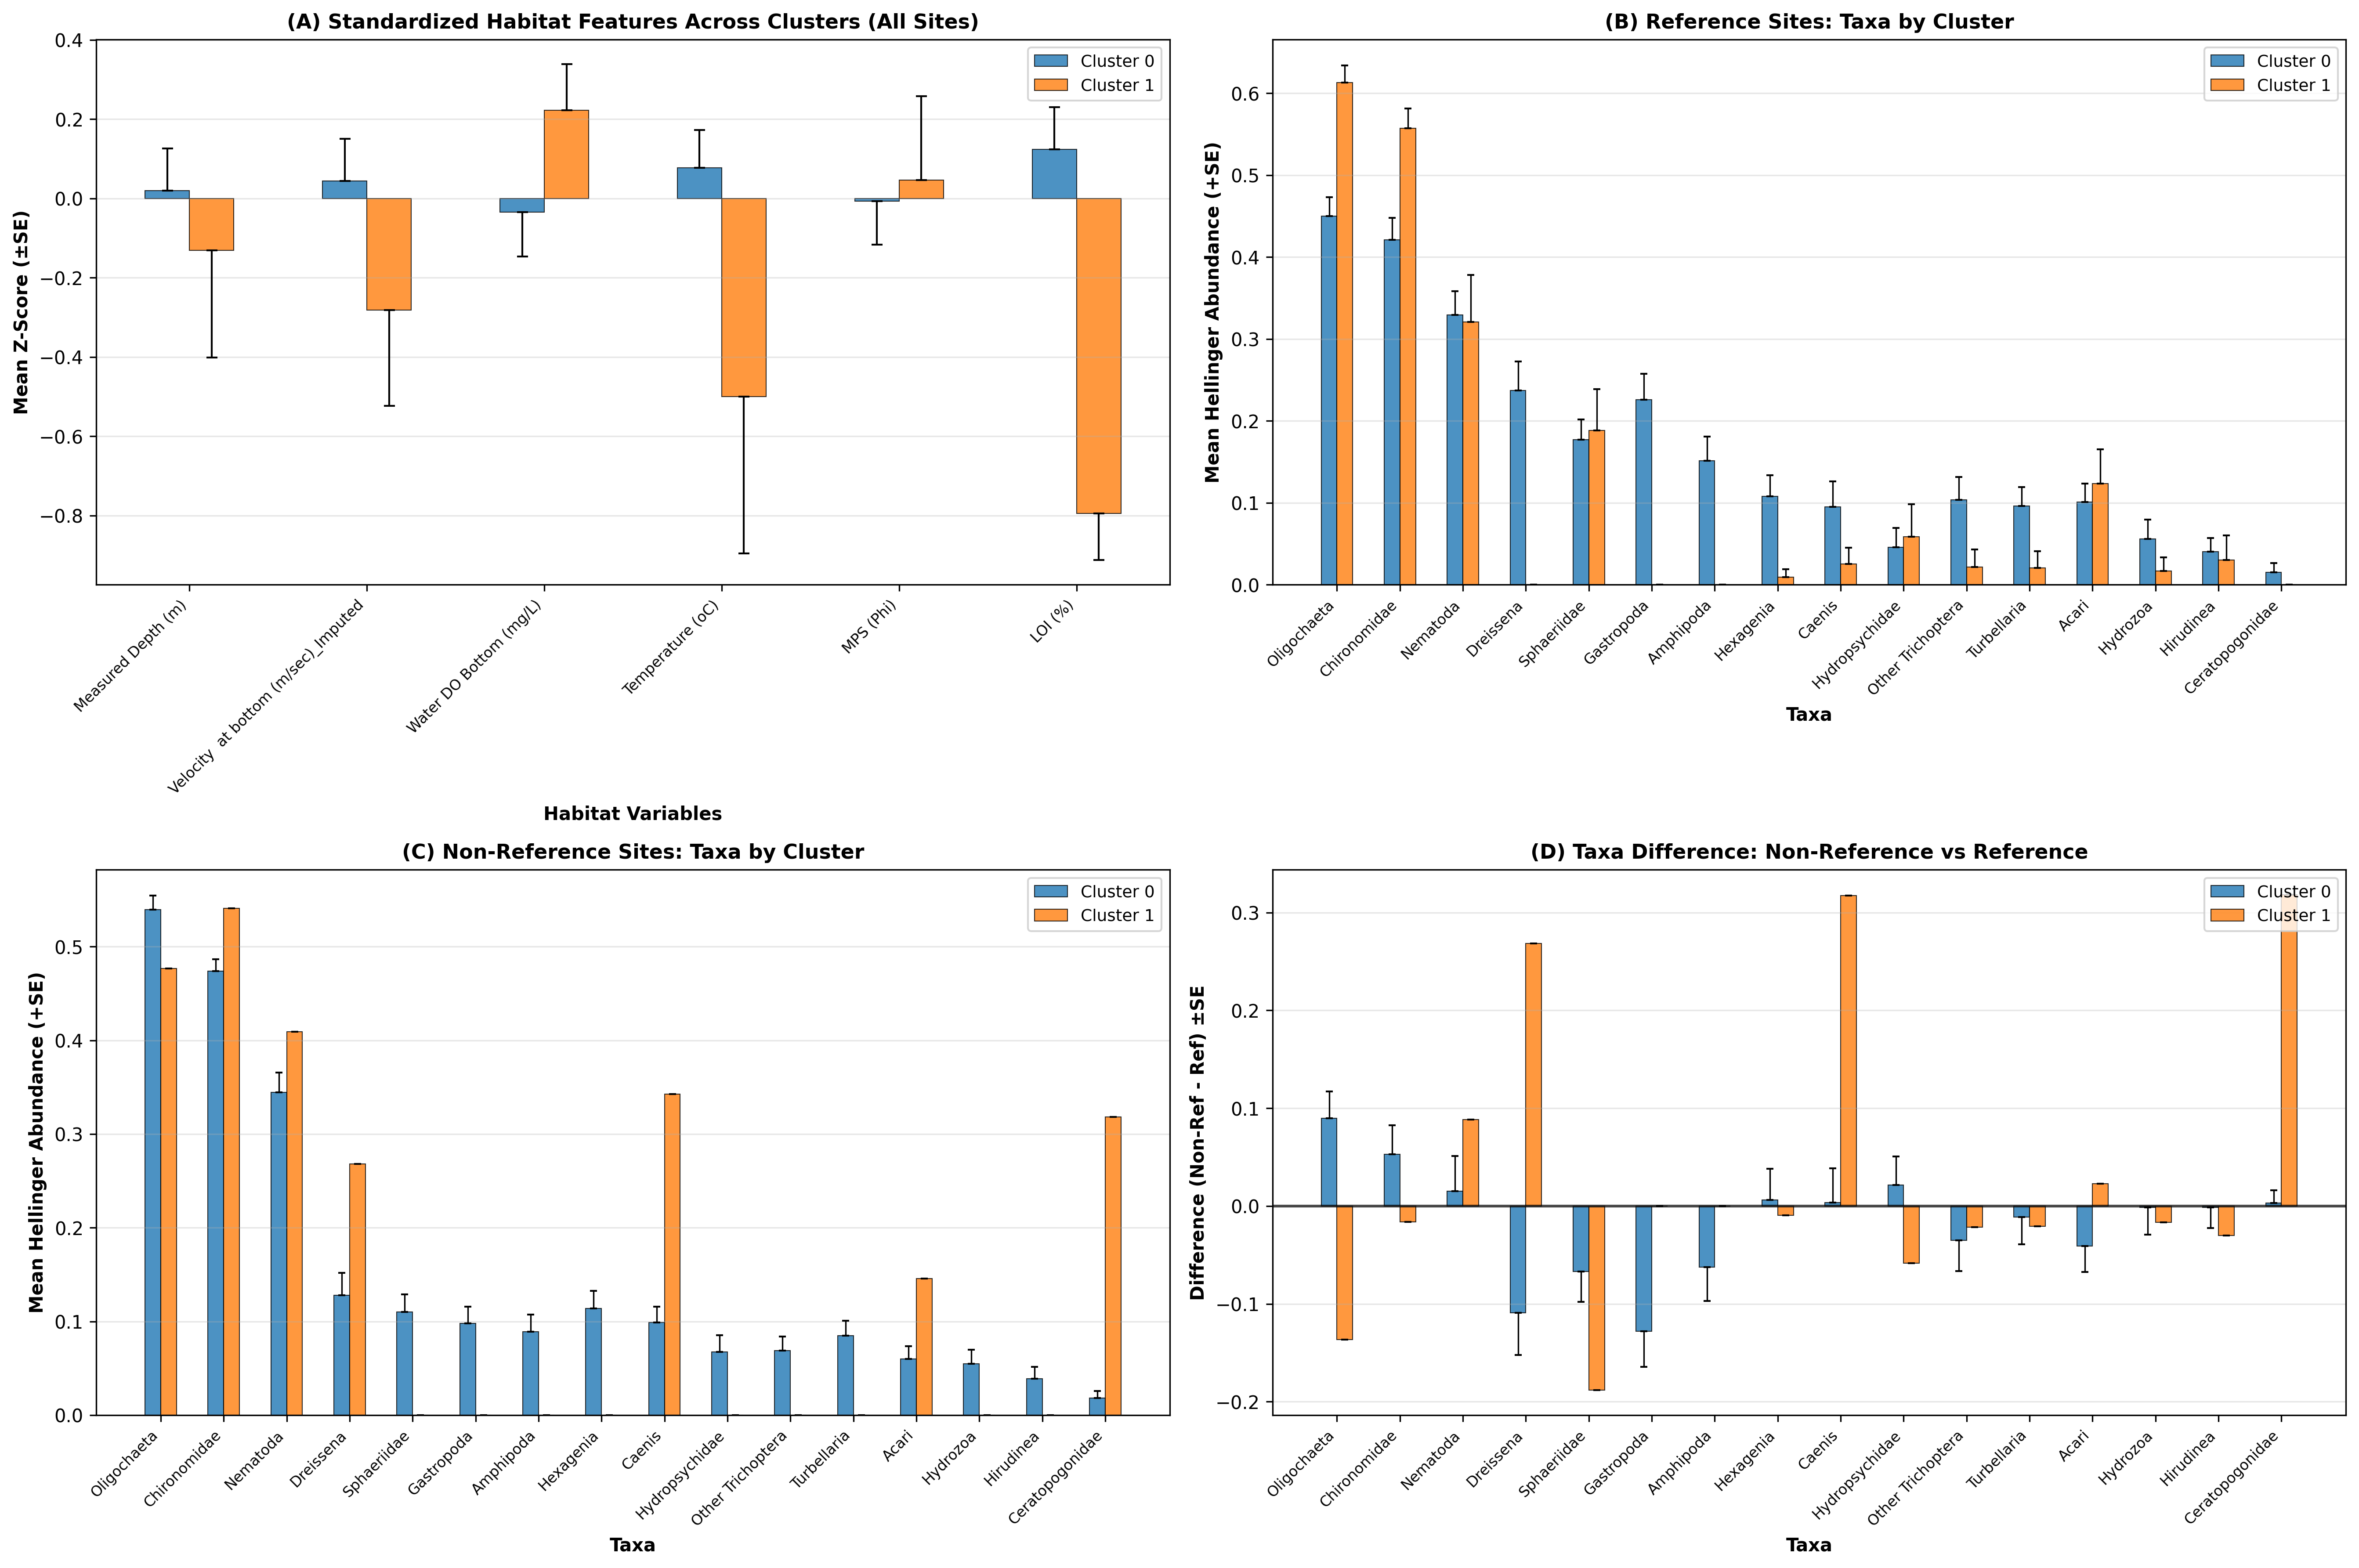
\includegraphics[width=0.9\textwidth]{../results/figures/03_env_driven_taxa_clusters/figure4_cluster_comparison.png}
    \caption{Cluster Comparison}
    \label{fig:03_cluster_comparison}
\end{figure}


\chapter{Community Composition Measures}

%% ============================================
%% PC vs Pollution Score Regression Results
%% ============================================

\begin{table}[htbp]
    \centering
    \caption{Significant Species PC vs Pollution Score Regressions}
    \label{tab:04_pc_pollution_regression}
    \small
    \begin{tabular}{cclccccc}
        \toprule
        \textbf{Cluster} & \textbf{PC} & \textbf{Var.(\%)} & \textbf{$R^2$} & \textbf{$\bar{R}^2$} & \textbf{Coef.} & \textbf{$t$-stat} & \textbf{$n$} \\
        \midrule
        0 & PC2 & 13.42 & 0.4223 & 0.4016 & $-0.0594$ & $-4.524^{***}$ & 30 \\
        2 & PC1 & 35.16 & 0.5039 & 0.4625 & $-0.0907$ & $-3.491^{**}$ & 14 \\
        \bottomrule
    \end{tabular}
    
    \vspace{0.5em}
    \footnotesize
    \textit{Note:} Only significant regressions shown ($p < 0.01$).
    Significance: $^{**}p < 0.01$; $^{***}p < 0.001$
\end{table}

%% ============================================
%% Pollution PC vs Species PC Regression Results
%% ============================================

\begin{table}[htbp]
    \centering
    \caption{Significant Pollution PC vs Species PC Regressions ($p < 0.05$)}
    \label{tab:04_pollution_pc_species_pc}
    \small
    \begin{tabular}{ccccccc}
        \toprule
        \textbf{Cluster} & \textbf{Poll. PC} & \textbf{Spec. PC} & \textbf{Var.(\%)} & \textbf{$R^2$} & \textbf{Slope} & \textbf{$n$} \\
        \midrule
        2 & PC2 & PC1 & 35.16 & 0.4321 & $-0.151^{*}$ & 14 \\
        0 & PC3 & PC2 & 13.42 & 0.2800 & $-0.159^{**}$ & 30 \\
        0 & PC4 & PC5 & 8.46 & 0.2600 & $-0.097^{**}$ & 30 \\
        0 & PC2 & PC2 & 13.42 & 0.2063 & $-0.096^{*}$ & 30 \\
        0 & PC2 & PC4 & 9.81 & 0.1594 & $0.072^{*}$ & 30 \\
        1 & PC2 & PC1 & 19.35 & 0.1172 & $0.085^{**}$ & 60 \\
        1 & PC1 & PC2 & 15.06 & 0.1025 & $-0.057^{*}$ & 60 \\
        1 & PC2 & PC6 & 6.40 & 0.0803 & $-0.041^{*}$ & 60 \\
        \bottomrule
    \end{tabular}
    
    \vspace{0.5em}
    \footnotesize
    \textit{Note:} Var.(\%) = variance explained by the Species PC. \\
    \textit{Poll. PC = Pollution Principal Component; Spec. PC = Species Principal Component.} \\
    \textit{Significance: $^{*}p < 0.05$; $^{**}p < 0.01$}
    \end{table}



% \begin{figure}[htbp]
%     \centering
%     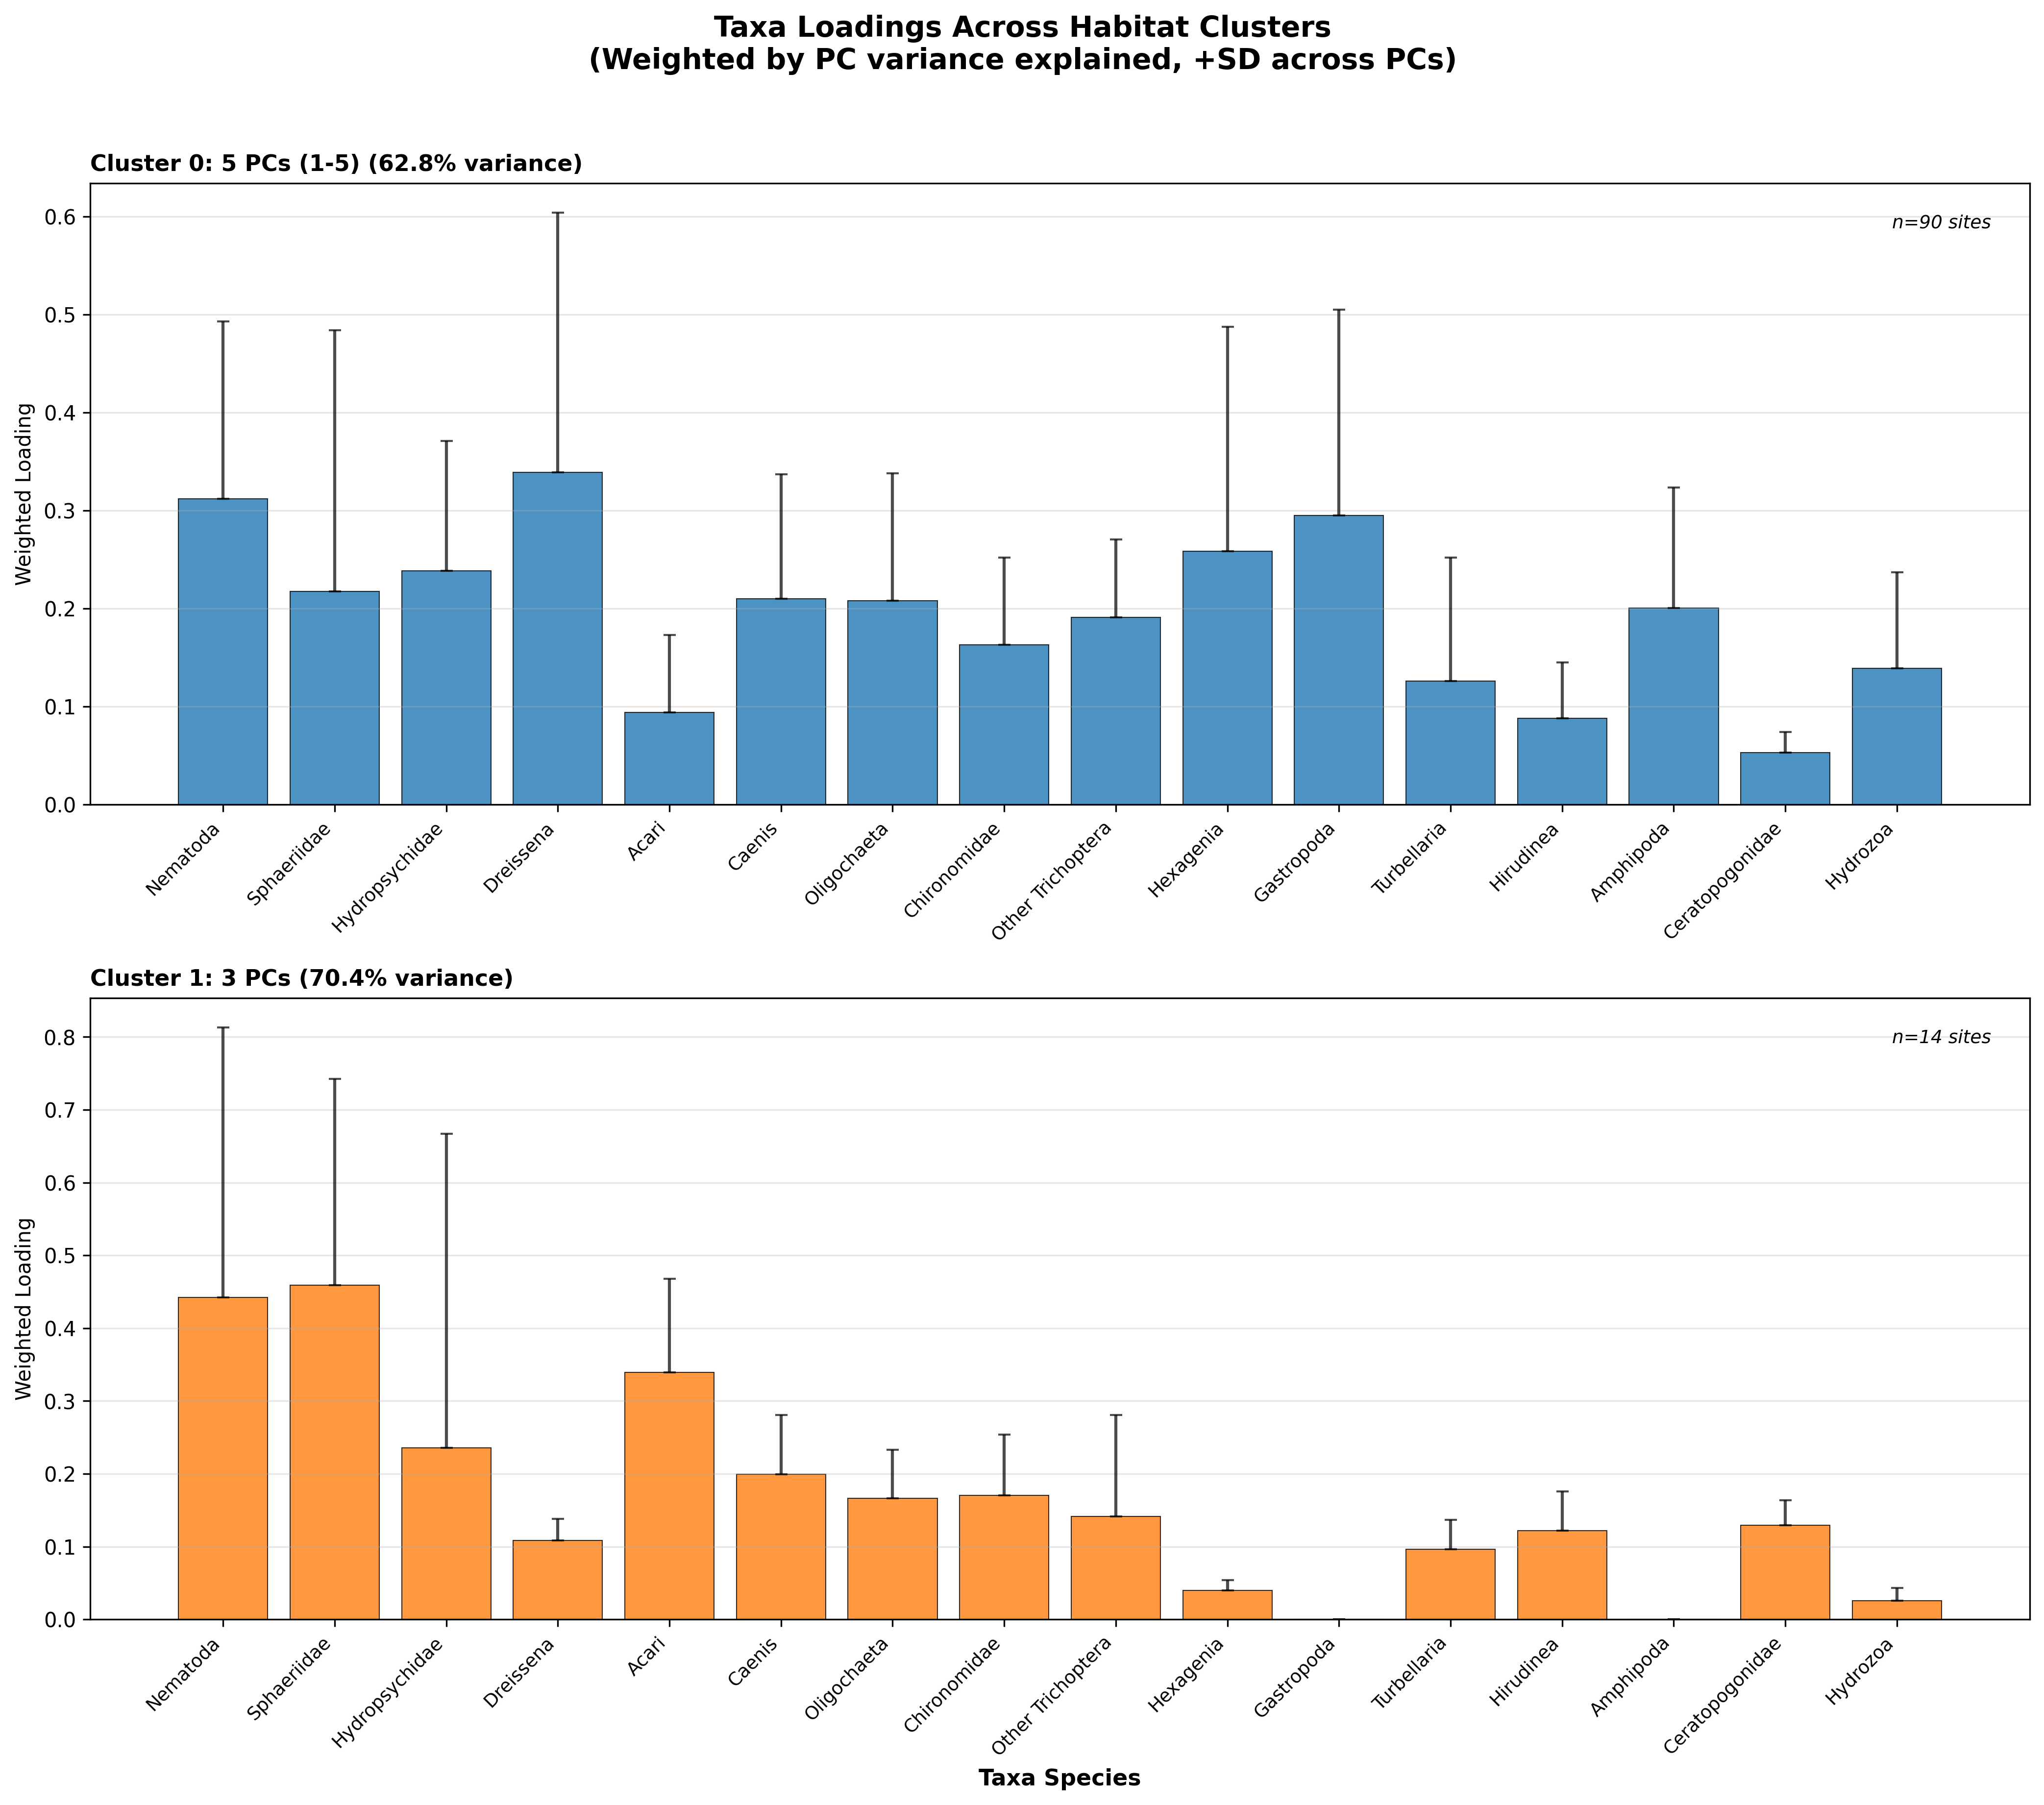
\includegraphics[width=0.9\textwidth]{../results/figures/04_community_composition_measures/figure1_taxa_loadings.png}
%     \caption{Taxa Loadings}
%     \label{fig:04_taxa_loadings}
% \end{figure}

\begin{figure}[htbp]
    \centering
    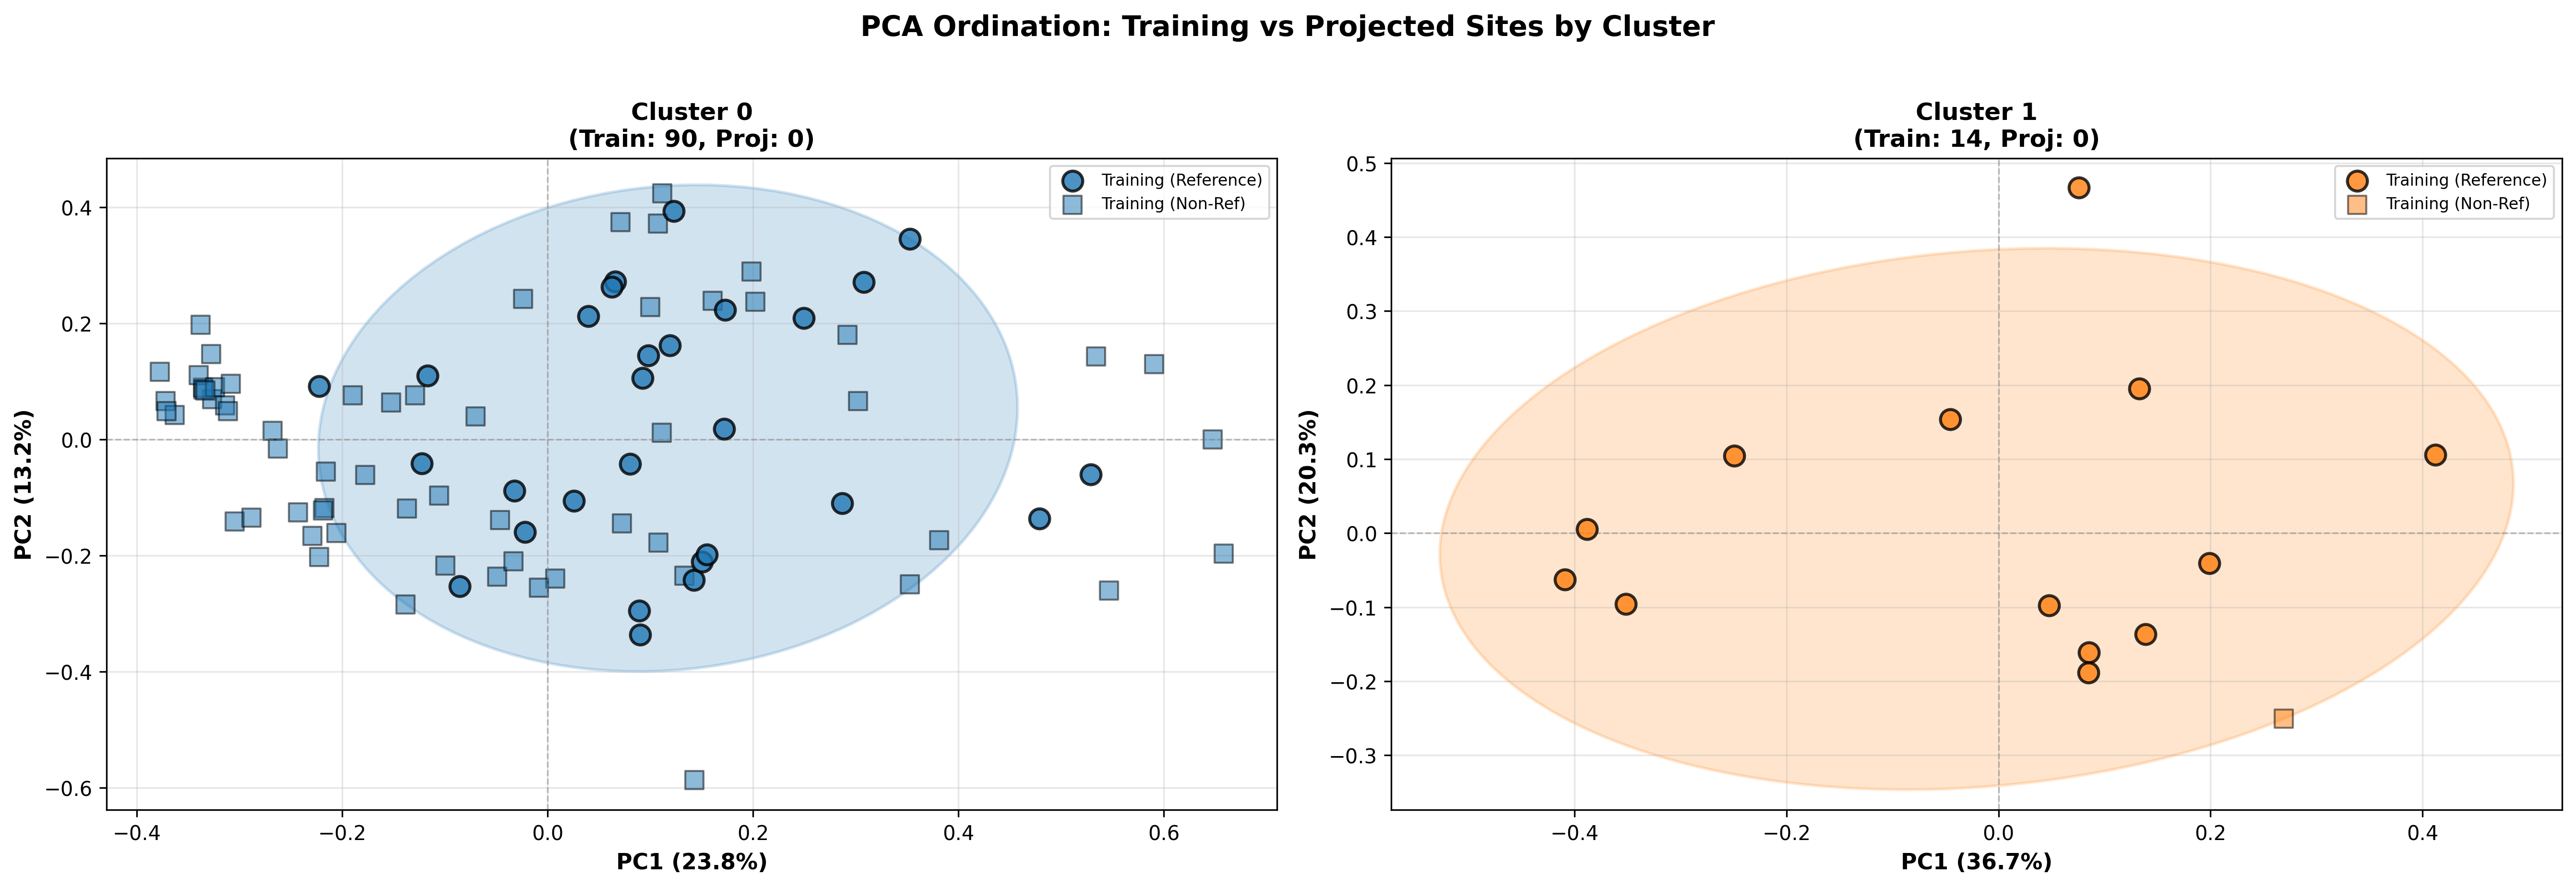
\includegraphics[width=0.9\textwidth]{../results/figures/04_community_composition_measures/figure2_ordination.png}
    \caption{Ordination}
    \label{fig:04_ordination}
\end{figure}

\begin{figure}[htbp]
    \centering
    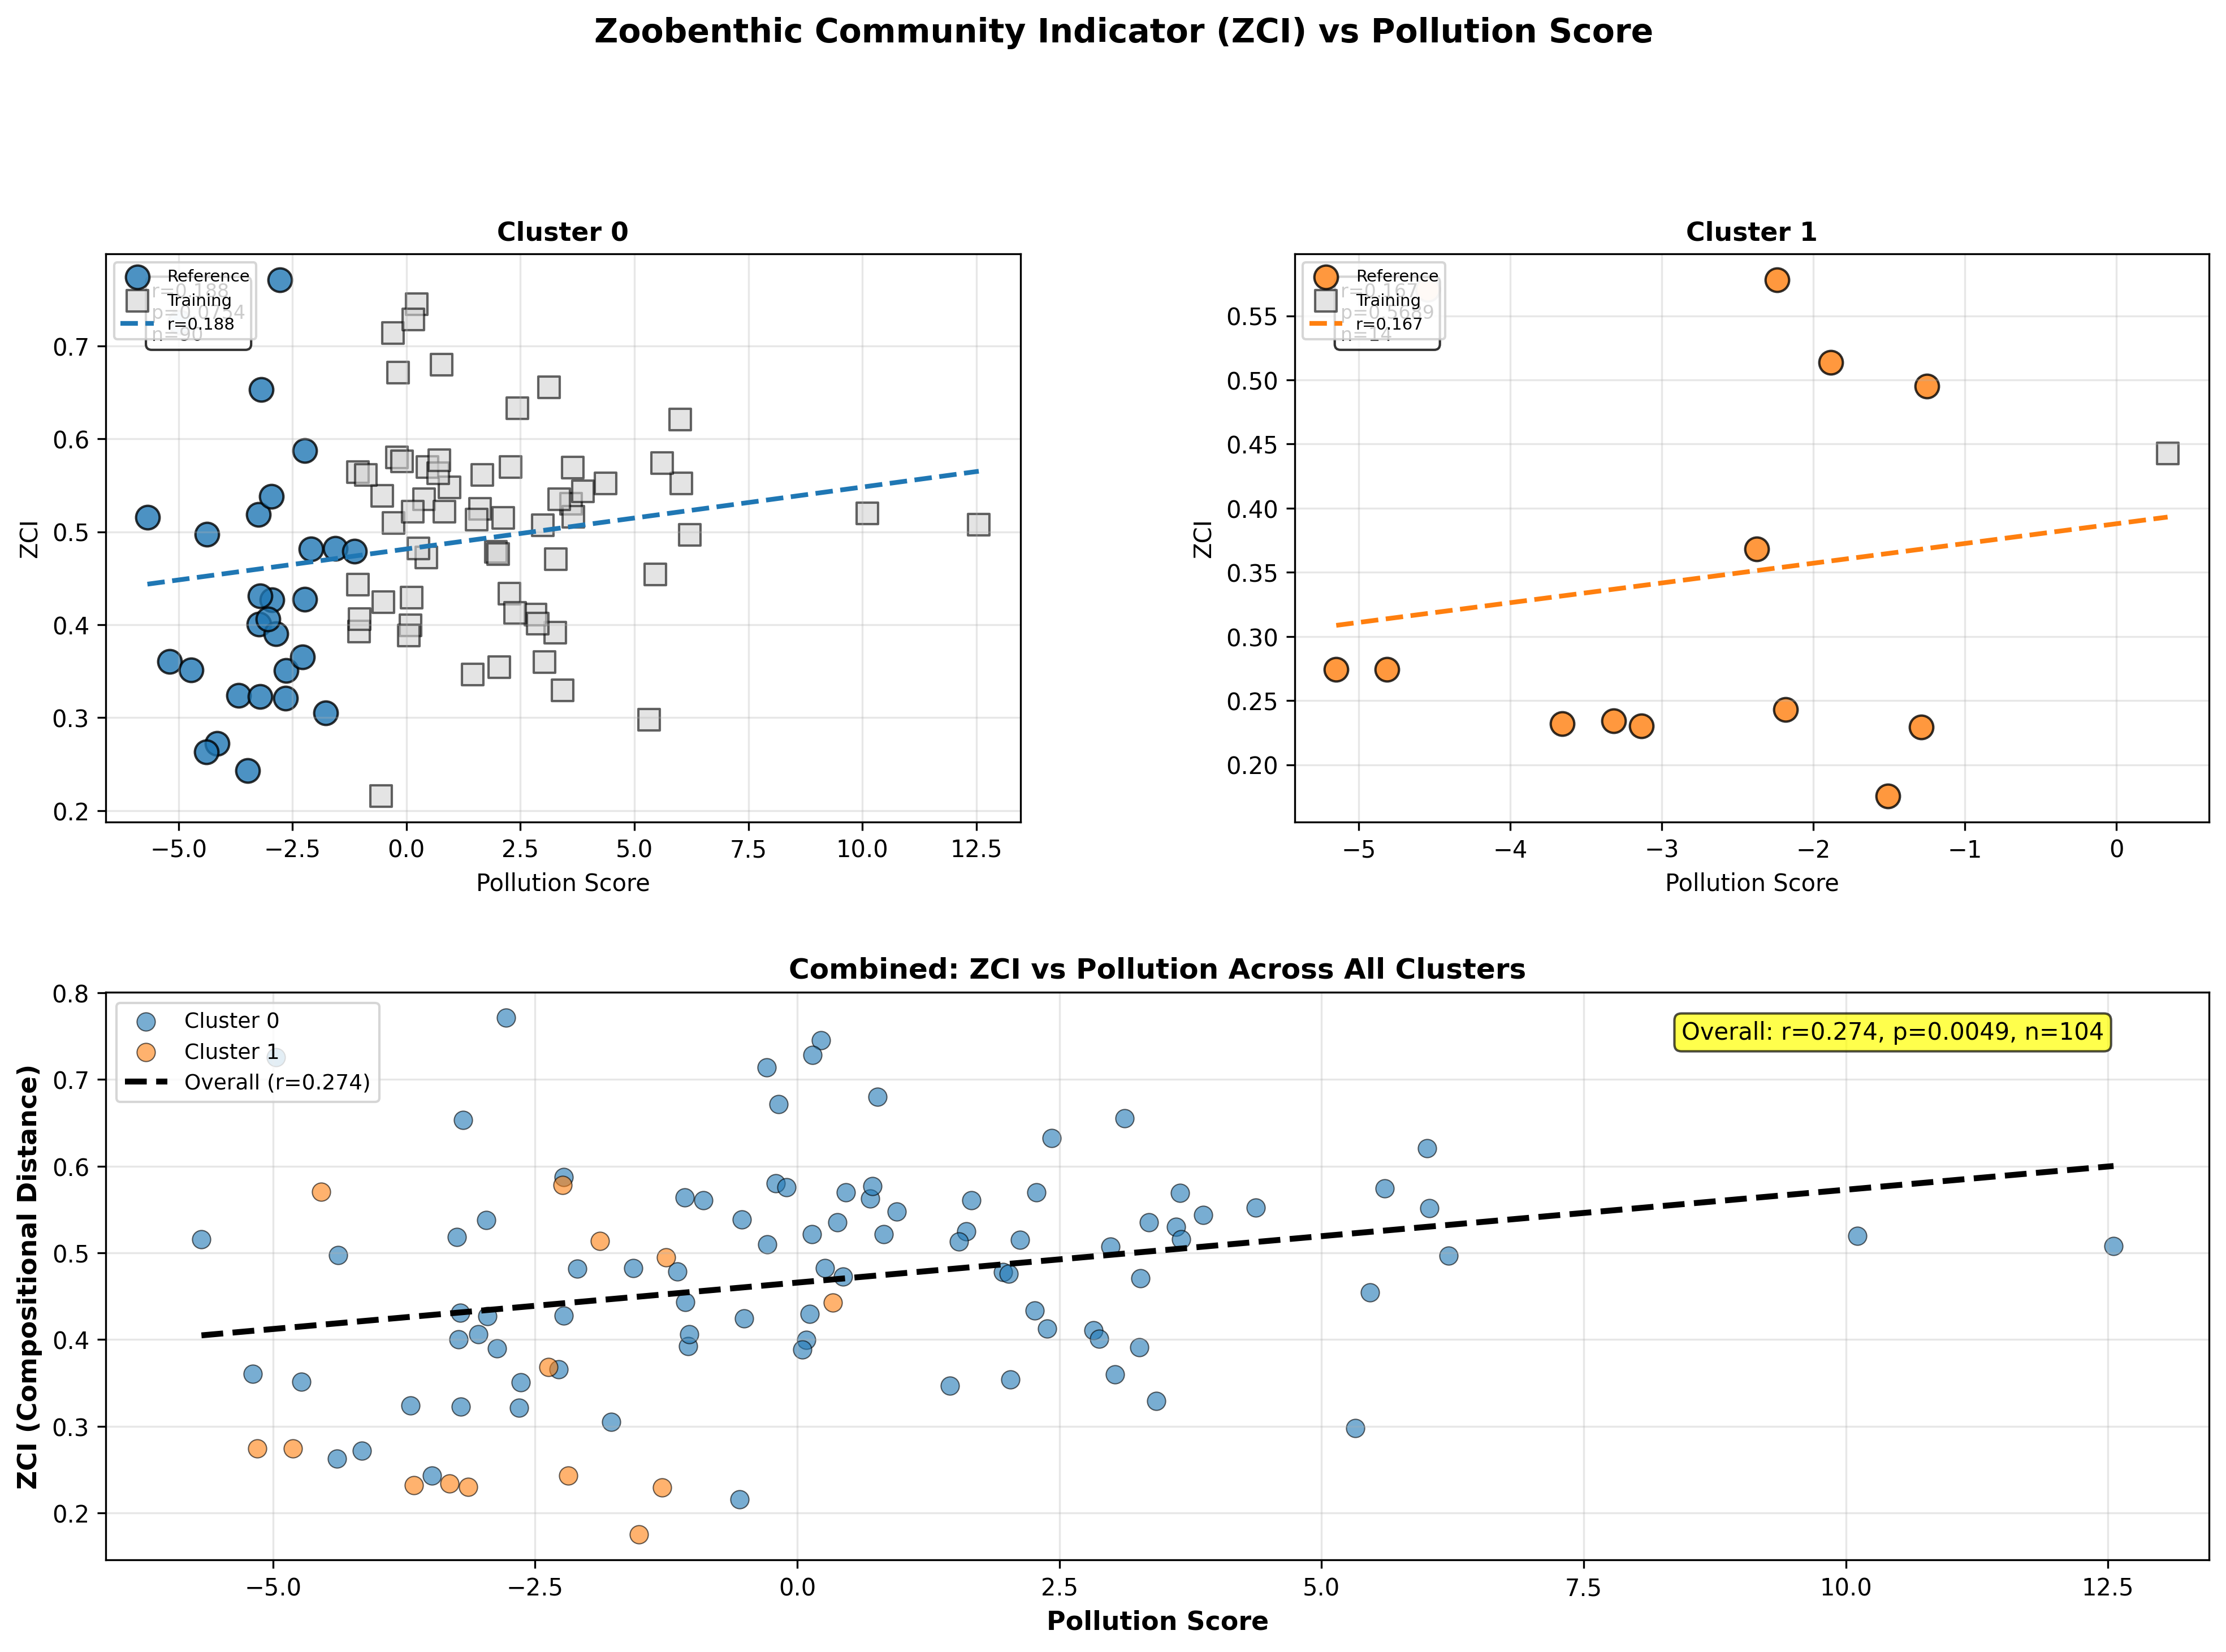
\includegraphics[width=0.9\textwidth]{../results/figures/04_community_composition_measures/figure3_zci_vs_pollution.png}
    \caption{ZCI vs Pollution}
    \label{fig:04_zci_vs_pollution}
\end{figure}

\begin{figure}[htbp]
    \centering
    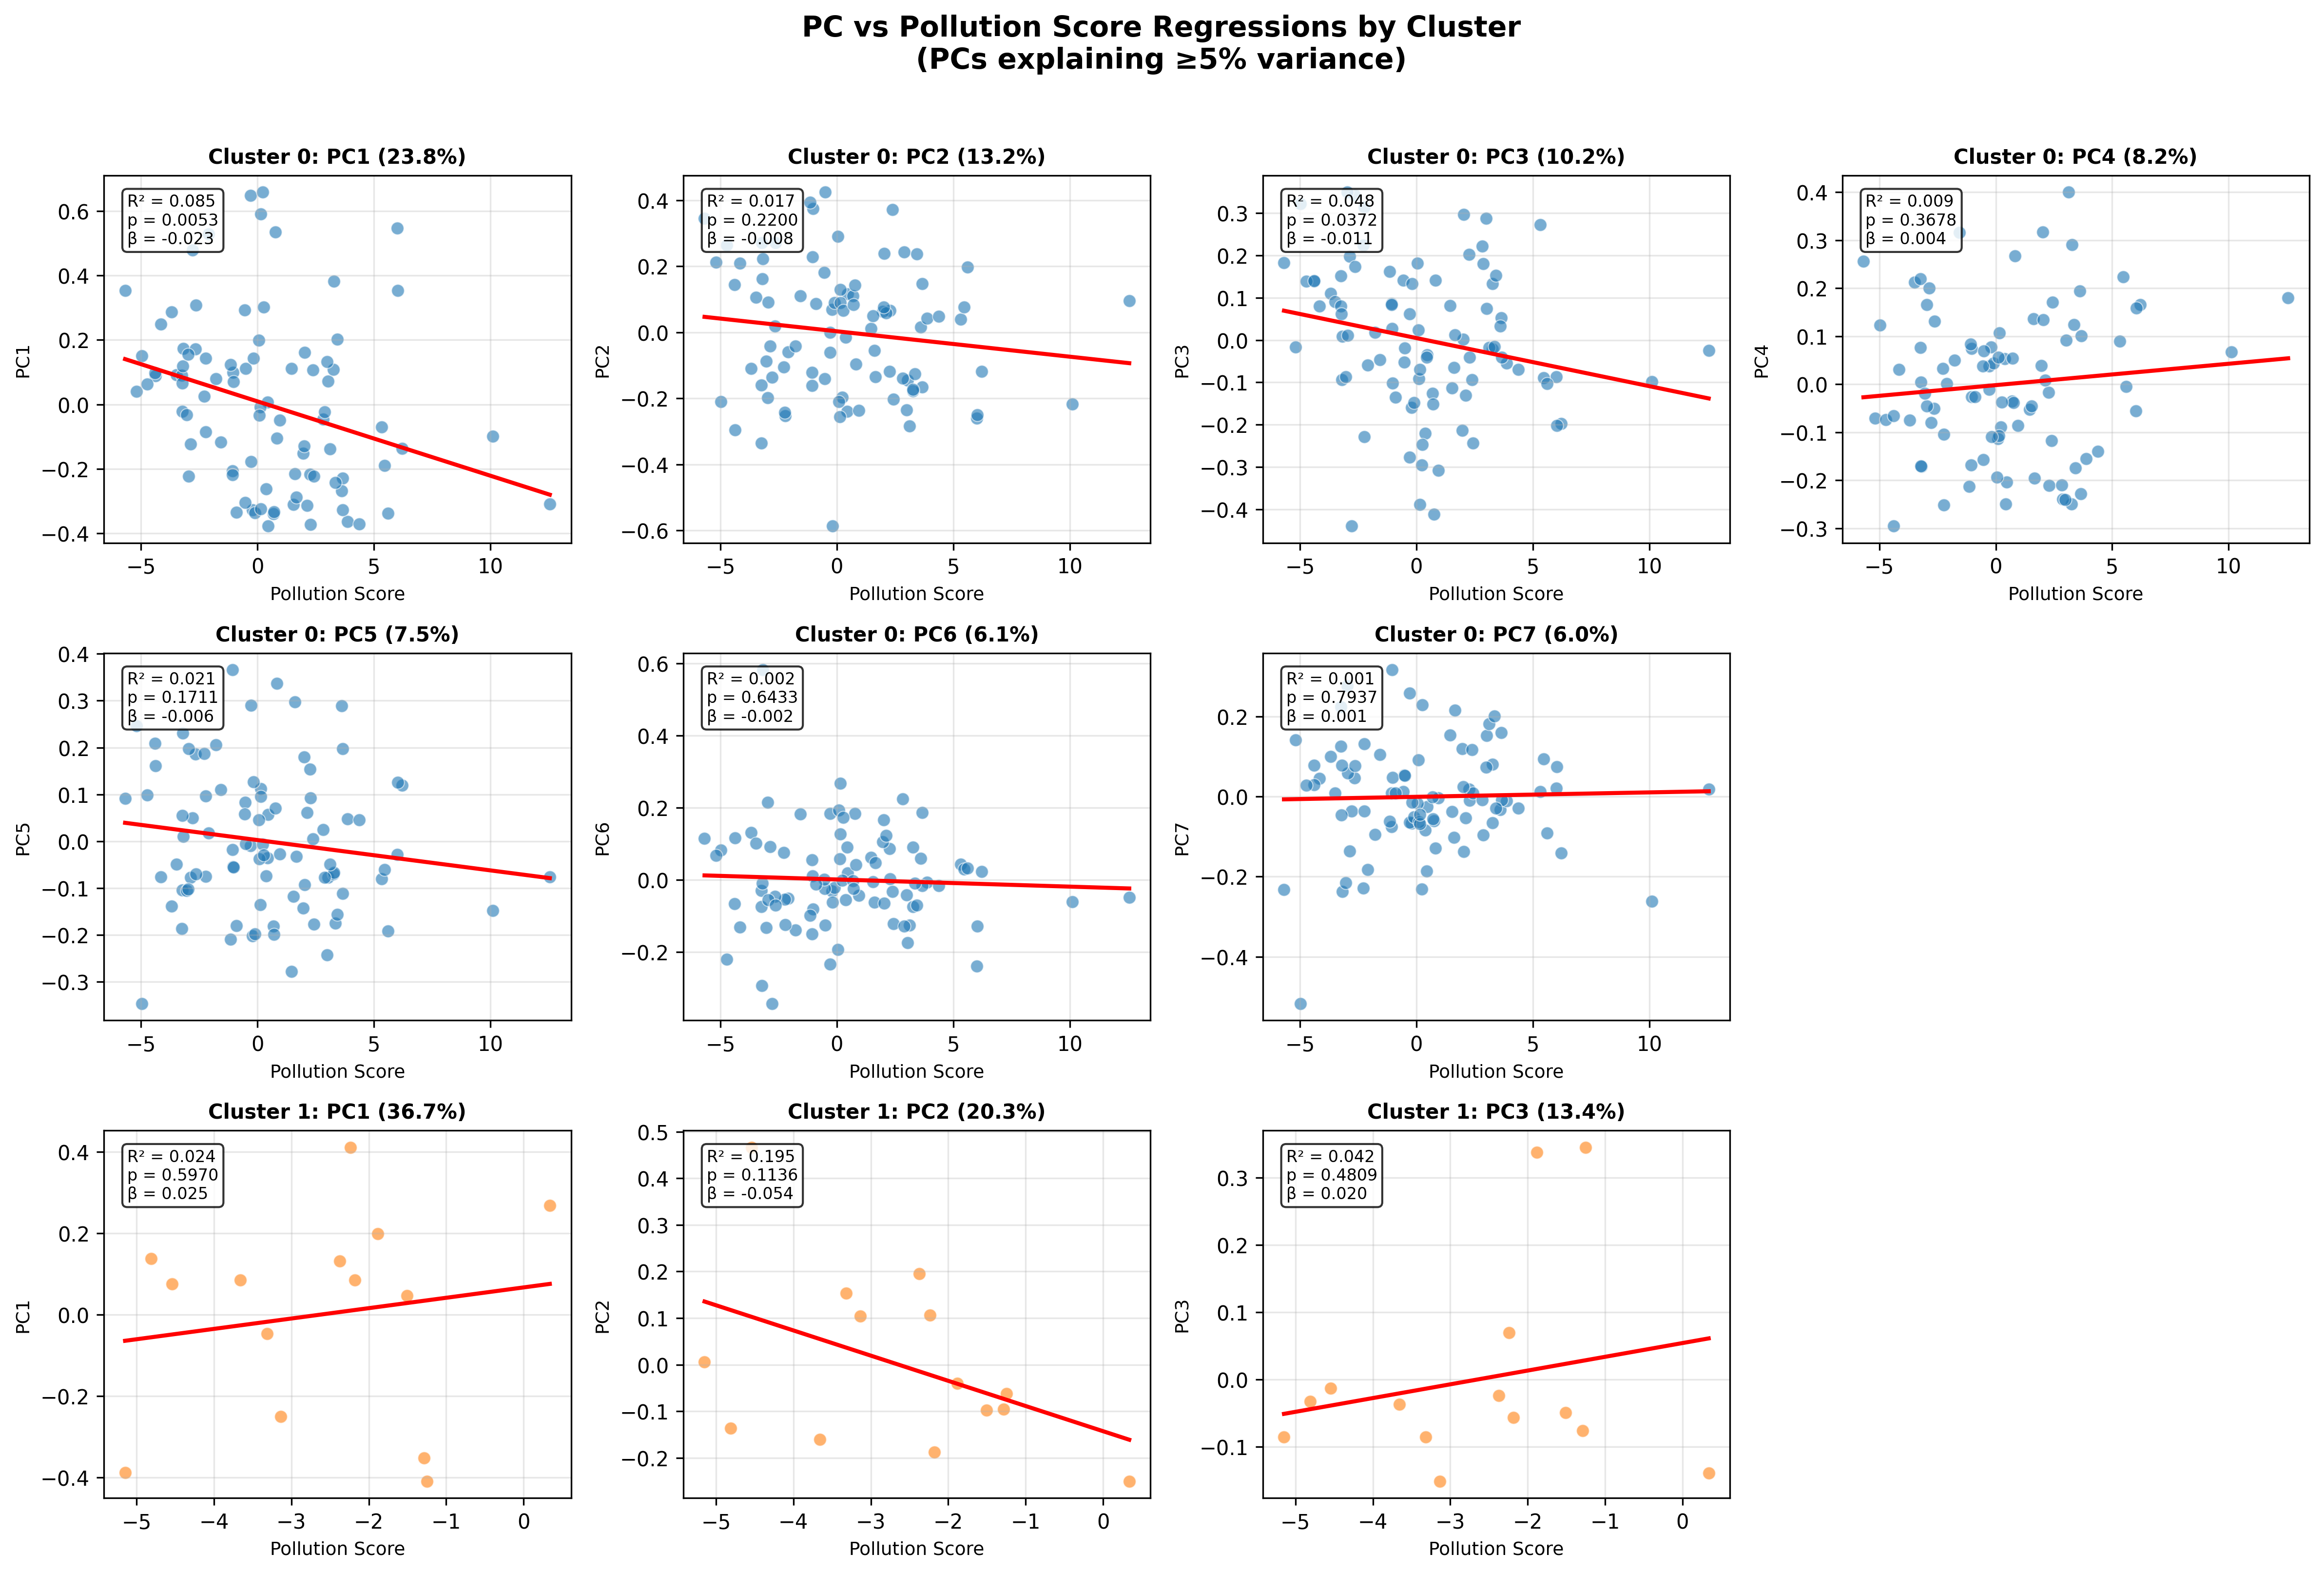
\includegraphics[width=0.9\textwidth]{../results/figures/04_community_composition_measures/figure4_pc_regression.png}
    \caption{PC Regression}
    \label{fig:04_pc_regression}
\end{figure}

\begin{figure}[htbp]
    \centering
    \includegraphics[width=0.9\textwidth]{../results/figures/04_community_composition_measures/figure5_pollution_vs_species_pc.png}
    \caption{Pollution vs Species PC}
    \label{fig:04_pollution_vs_species_pc}
\end{figure}


\clearpage
\bibliographystyle{plain}  % or use unsrt if you want citations in order of appearance
\bibliography{sections/Reference}   % your .bib file, without .bib extension

\end{document}

